\documentclass[a4paper, 11pt]{article}
\usepackage{/Users/fgu/dev/projects/dotfiles/latex/paper}
\bibliography{/Users/fgu/dev/projects/dotfiles/latex/fabib}
\onehalfspacing

\newcommand{\figdir}{../../output/figures}
\newcommand{\tabdir}{../../output/tables}

\title{\textbf{Evaluation\footnote{This research was supported by Economic and Social Research Council grant number ES/V004867/1. WBS ethics code: E-414-01-20.}}}

\author{
    Fabian Gunzinger \\ Warwick Business School
    \and
    Neil Stewart \\ Warwick Business School
}

\date{\today}

\begin{document}

\maketitle
% % !TEX root = ../eval.tex

\begin{abstract}

In this paper, I test whether using Money Dashboard is associated with a
reduction in discretionary spending and an increase in ``emergency savings''. I
find that users reduce their discretionary spend by between \pounds100 and
\pounds150 (11-17\% of average discretionary spend) once they start using the
app and sustain that reduction throughout the six-month post-signup period I
consider. In contrast, I cannot find an increase in short-term or long-term
savings. Looking at disaggregated measures of discretionary spend further
suggests that the reduction in spend is the result of maintained month-to-month
changes in behaviour rather than one-off cancellations of direct-debit
transactions, that it results from reductions across a number of spending
categories, and that it is a result of changes along the extensive rather than
the intensive margin -- users reduce the number of transactions they make
rather than the average transaction value.

\end{abstract}



\tableofcontents
\newpage

% % !TEX root = ../eval.tex

\section{Introduction}%
\label{sec:introduction}

This paper evaluates whether Money Dashboard, a UK-based financial aggregator
app, helps its users reduce their discretionary spend and increase their
``rainy-day savings''.

The question is important because a large number of adults in the UK and the US
do not have enough savings to cover unexpected expenses like car or medical
bills: in the UK, 25 percent of adults would be unable to cover an unexpected
bill of \pounds300 \citep{philipps2021supporting}, while in the US, about 30
percent would be unable to cover a \$400 bill \citep{fed2022economic}. But
while there is a large body of research that studies reasons for why savings
are low, little is known about what could help people save
more.\footnote{Well-documented behavioural biases that help explain undersaving
    are, among others, present bias \citep{laibson1997golden,
    laibson2019intertemporal}, inertia \citep{madrian2001power},
    over-extrapolation \citep{choi2009reinforcement}, and limited self-control
    and willpower \citep{thaler1981economic, benhabib2005modeling,
    fudenberg2006dual, loewenstein2004animal, gul2001temptation}. One danger of
    viewing low savings mainly as a result of behavioural biases is that while
    these biases likely do play some role and designing environments and tools
    to help correct them are thus part of the solution, it is at least
    conceivable that this is an area where the focus on behaviour-level
    solutions distracts from an effort to find more effective society-level
    solutions, a danger inherent in behavioural science research convincingly
    highlighted in \citet{chater2022frame}: if the main problem is that many
people are unable to earn enough to save, then the effectiveness of helping
them manage their low incomes more effectively pales in comparison with efforts
to help them earn more.}

FinTech aggregator apps like Money Dashboard are promising because they provide
easy access to financial information that make it easier to monitor ones
spending and saving, and often also offer tools such as budgeting and the
setting of spending goals. Financial information that
is more easily accessible and is aggregated in ways that help people keep track
of their goals might be beneficial because rational inattention theory predicts
that it makes people more likely to access that information, which, in turn,
might lead to better consumption decisions. Similarly, tools that help with
budgeting and with setting spending goals have the potential to help users make
consumption decisions more in line with their intentions because such tools can
act as commitment devices that -- if users experience disutility from falling
short of their goals -- introduce a cognitive cost to overspending or
undersaving.\footnote{On rational inattention theory, see, for instance,
    \citet{brunnermeier2008wealth, dellavigna2009psychology,
    sims2003implications}.  On commitment devices see, among others,
    \citet{thaler1981economic, laibson1997golden, o1999doing} for theoretical
    foundations, and \citet{beshears2016beyond, hsiaw2013goal} for a discussion
of soft commitment devices.}

The nascent literature that studies the effect of FinTech apps on financial
outcomes suggests that these apps can indeed lead to improved financial
outcomes: they have been found to reduce spending by providing users with
information about their spending relative to peers
\citep{dacunto2020crowdsourcing} and offering budgeting options
\citep{lukas2022influence}, to increase savings by offering budgeting options
\citep{gargano2021goal}, and to reduce non-sufficient fund fees by facilitating
access to information \citep{carlin2022mobile}.

In this paper, I specifically test whether using Money Dashboard is associated
with a reduction in discretionary spending and an increase in ``rainy-day
savings''. I use a new estimator proposed by \citet{callaway2021difference}
that corrects for recently identified problems in two-way fixed effects
estimates.

\edit{I find...}

There are two main limitations to the approach. First, the data is not
generated by a randomised experiment. The gold-standard to evaluate whether use
of Money Dashboard improves financial outcomes would be a randomised
controlled-trial, where out of a sample of potential users (ideally random and
representative of the UK population), we would randomly grant access to the app
to some users and then compare outcomes of those treated users with the control
group of users who did not have access.  Instead, the data I have access to
only contains data for individuals who self-selected into using the app.
Individuals will choose to do so for a number of different reasons, all of
which are unobserved in the data, and at least some of which would probably
have changed their financial outcomes even if they had not signed up to the
app. Any changes in financial outcomes we observe are thus ``aggregate'' or
``net'' effects of these unobservables and the ``pure'' causal effect of app
use.

To see this, think of the net effect as $\textit{net effect} = \textit{causal
effect} + \textit{``need''}(\downarrow) + \textit{``motivation''}(\uparrow)$,
where the arrows indicate the direction of the bias, and consider three cases
that illustrate three stylised but plausible scenarios for signup. First,
consider a user who signs up in the hope that the app will help them reign in
discretionary spending that has has gotten out of hand. If it takes the user
some time to fully adjust their spending, then even if the app does help them
make these adjustments, the estimated positive effect of app use will be biased
downward. Next, consider a user who decides to start bringing their own lunch
to work instead of eating out in an effort to save for a new car and signs up
to MDB in the hope that the app will help them keep track of their spending.
Such a user would probably have reduced their discretionary spend even if they
had not signed up to the app, thus creating an upward bias on our estimated net
effect. Finally, consider a user who signs up to MDB purely because they
happened to see an advert for the app on the Bus and got curious. In this case,
we can think of signup being close to random -- almost as if the user had been
allocated to the treatment group in our ideal experiment -- and the estimated
net effect will closely resemble the causal effect of app use. Hence, under the
weak assumption that at least some users sign up for reasons that are not as
good as random, our estimated effects will be biased upwards or downwards
depending on the relative proportion of users whose unobservable reasons for
signup create an upward and downward bias.

The second limitation is that even if I were able to isolate the effect of
the app, I am not able to differentiate between the contributions of different
features of the app such as improved access to information and budgeting.

\edit{However, despite these limitations, the results tell us... suggest that
further research is worthwhile}

My work mainly contributes to three strands of the literature. The first, is the
aforementioned recent literature that studies the effect of FinTech apps on
financial outcomes. The second, is the very recent literature on studying
interventions to help increase ``rainy-day savings'' an area of household
finances that has until recently had no attention. In addition to studies
testing the effect of FinTech apps on savings, there is a strand of research
that studies the use of auto-enrolment into employer-sponsored savings accounts
-- similar to the ones used to increase pension savings \citep{thaler2004save,
choi2004better, choukhmane2019default} -- and finds an increase in both
participation (relative to opt-in accounts) and account balances
\citep{beshears2020building, berk2022automating}. Finally, my work also
contributes to a rapidly growing literature of using financial-transaction data
from banks or financial aggregator apps to understand consumer financial
behaviour. As already mentioned, \citet{kuchler2020sticking} use data from a
financial aggregator app to estimate time preferences. Similar data has been
used to show that consumer spending varies across the pay cycle
\citep{gelman2014harnessing,olafsson2018liquid}, to test the consumer spending
response to exogenous shocks \citep{baker2018debt,baugh2014disentangling}, and
to better understand the generational differences in financial platform usage
patterns \citep{carlin2019generational}. Some researchers use transaction-data
directly provided by banks. \citet{ganong2019consumer} show that consumer
spending drops sharply after the predictable income drop from exhausting
unemployment insurance benefits, \citet{meyer2018fully} analyse how individuals
reinvest realised capital gains and losses, and \citet{muggleton2020evidence}
show that chaotic spending behaviour is a harbinger of financial distress.

To make it easier for interested readers to clarify questions about details and
subtleties of data preprocessing and analysis steps, I provide links to the
scripts that implement the steps discussed in the text in the relevant places
throughout the text. The links are indicated with the GitHub logo (\faGithub).
The projects GitHub repo that contains all files used to produce the results
can be found at
\href{https://github.com/fabiangunzinger/mdb\_eval}{https://github.com/fabiangunzinger/mdb\_eval}.

The remainder of this paper is organised as follows: Section~\ref{sec:data}
introduces the dataset used, discusses preprocessing and presents summary
statistics; Section~\ref{sec:estimation} introduces the empirical approach used
in the analysis; Section~\ref{sec:results} presents the results; and
Section~\ref{sec:conclusion} concludes.

\section{Introduction}%
\label{sec:introduction}


% % !TEX root = ../eval.tex

\section{Methods}%
\label{sec:data}

\subsection{Dataset}%
\label{sub:dataset}

\begin{itemize}

    \item Money Dashboard can access up to three years of historic data for
        each account a user links to their account.

    \item Each user for whom we have sufficient data thus serves as both a
        treatment unit and a potential control unit.

    \item Limitations: We have more data for users that signed up later. So average user in
        the study is not the average MDB user. If time of signup is mainly
        driven by financial savyness, then study sample is closer to overall
        population than MDB sample (if we rank groups as early joiners > late
        joiners > never joiners in terms of financial sophistication). If,
        however, signup reflects something like openness to newness, then it's
        not necessarily correlated with financial savyness. Either way, we
        might ignore it for now. We could test whether behaviour differs
        between early or late adopters, but that doesn't seem important enough.

\end{itemize}

\subsection{Data preprocessing}%
\label{sub:data_preprocessing}

\paragraph{Cleaning}%
\label{par:cleaning}

MDB cleaning (mdb/mdb/clean.py)
\begin{itemize}
    \item About 75 percent of transactions are not automatically categorised,
        and we drop transactions that have no automatic tag. Dropping untagged
        transactions means that we might underestimate spending and savings,
        but entures that we do not miscategorise transactions.

    \item Custom tag classifications.

    \item Drop transactions for which user ID, account ID, date, amount, and
        transaction description are identical. This will drop some genuine
        transactions, such as someone buying two identical cups of coffees at
        the same coffee shop on the same day. However, data inspection suggests
        that in most cases, we remove genuine duplicates.
\end{itemize}


\paragraph{Sample selection}%
\label{par:sample_selection}

We select our sample so as to include users for whom we can be reasonably
certain that we observe all relevant financial transactions, and do so for at
least six months before and after they sign up to the app. In addition to that,
we exclude users who might use the app for business purposes as well as
pensioneers, whose financial objectives might be different.

\begin{table}
\centering
\caption{Sample selection}\label{tab:selection}
\begin{tabular}{lrrrr}
\toprule
                                       &  Users & User-months &       Txns & Txns (m\pounds) \\
\midrule
                            Raw sample & 27,175 &     795,338 & 65,972,558 &          12,527 \\
             Drop first and last month & 26,565 &     741,170 & 64,157,932 &          12,179 \\
  At least 6 months of pre-signup data & 11,835 &     310,517 & 29,244,871 &           5,743 \\
 At least 6 months of post-signup data &  6,404 &     195,050 & 19,681,242 &           3,957 \\
          At least one current account &  5,833 &     178,845 & 18,257,300 &           3,738 \\
          At least one savings account &  4,506 &     138,181 & 14,485,916 &           3,133 \\
At least \pounds5,000 of annual income &  1,877 &      57,064 &  6,493,155 &           1,386 \\
           At least 10 txns each month &  1,686 &      51,190 &  5,935,336 &           1,262 \\
  At least \pounds200 of monthly spend &  1,478 &      44,641 &  5,333,532 &           1,135 \\
      Complete demographic information &  1,240 &      38,087 &  4,598,590 &             952 \\
                           Working age &  1,219 &      37,377 &  4,529,599 &             929 \\
                          Final sample &  1,219 &      37,377 &  4,529,599 &             929 \\
\bottomrule
\end{tabular}

\tabnote{\textwidth}{Number of users, user-months, transactions, and
transaction volume in millions of British Pounds left in our sample after each sample selection step. Link to sample selection
code:
\href{https://github.com/fabiangunzinger/mdb_eval/blob/main/src/data/selectors.py}{\faGithub}.}
\end{table}


Table~\ref{tab:selection} lists the precise conditions we applied to implement
these criteria and their effect on sample size. We remove the first and last
month of data for all users because we are unlikely to observe all transactions
for these months. We also drop test users, since their objectives for app use
might have been different from ordinary users.\footnote{We cannot identify test
users precisely, but drop users who signed up prior to or during the first year
the app was in operation.}

To ensure that we observe users for at least 12 months around app signup, we
require 6 months of data before the signup month, and another five months after
the signup month. Our main outcome variable is netflows into a user's savings
accounts. It is thus critical that we observe enough historical data for these
savings accounts to ensure that we observe all transactions during our 12 month
perdiod of interest. This is complicated by the fact that we cannot see when an
account was opened at the bank, but only when it was added to the app. While
cases where a user adds an account to the app as soon as it was opened are
unproblematic, users will often add accounts after they were opened, either
because they have accounts that they opened before signing up to the app, or
because they opened new accounts after signup but add them to the app with a
delay. In such cases, it is critical that, once the account is added, we
observe the complete historical data up to 6 months before signup or up to the
month in which the account was opened, whichever happened later. To see why
this is critical, imagine a scenario where a user opens an account 10 months
before they sign up to the app, makes a monthly transfter to the account of
\pounds100, adds the account to the app on signup, but we onserve only 3 months
of historical data. In this case we would observe that the user saved
\pounds300 before signup and \pounds600 after, and erroneously conclude that
post signup savings were twice as high. The most extreme case we need to cover
is that of a user opening a savings account more than six months before signup
and adding the account to the app five months after signup, in which case we
need to be sure to observe 12 months of historical data. As shown in
Appendix~\ref{app:data}, all major banks started providing 12 months of
historical data for current and savings accounts from April 2017 onwards, which
is why we restrict our sample to users who signed up in or after that month.

To ensure that we can be reasonably certain to observe users have added all
their financial accounts to the app, we restrict our sample to users with at
least one savings and current account, with an annual income of at least
\pounds5,000, and a minimum of 10 transactions and a spend of \pounds200 every
month. To remove users who might use the app for business purposes, we drop
users with more than 10 active accounts in any given month. Finally, we remove
users for whom we cannot observe all demographic information we use as
covariates in our analysis, and users who are not between the ages of 18 and
65, as their financial objectives are plausibly different.


\paragraph{Data transformations:}%
\label{par:data_transformations}

To minimise the influence of outliers, we winsorise spend, income, and savings
accounts flow variables at the 1 percent level or -- if we winsorise on both
ends of the distribution -- at the 0.5 percent level.


\subsection{Summary statistics}%
\label{sub:summary_statistics}

Figure~\ref{fig:sample_description} describes the sample.

\begin{figure}[H]
    \centering
    \caption{Sample characteristics}
    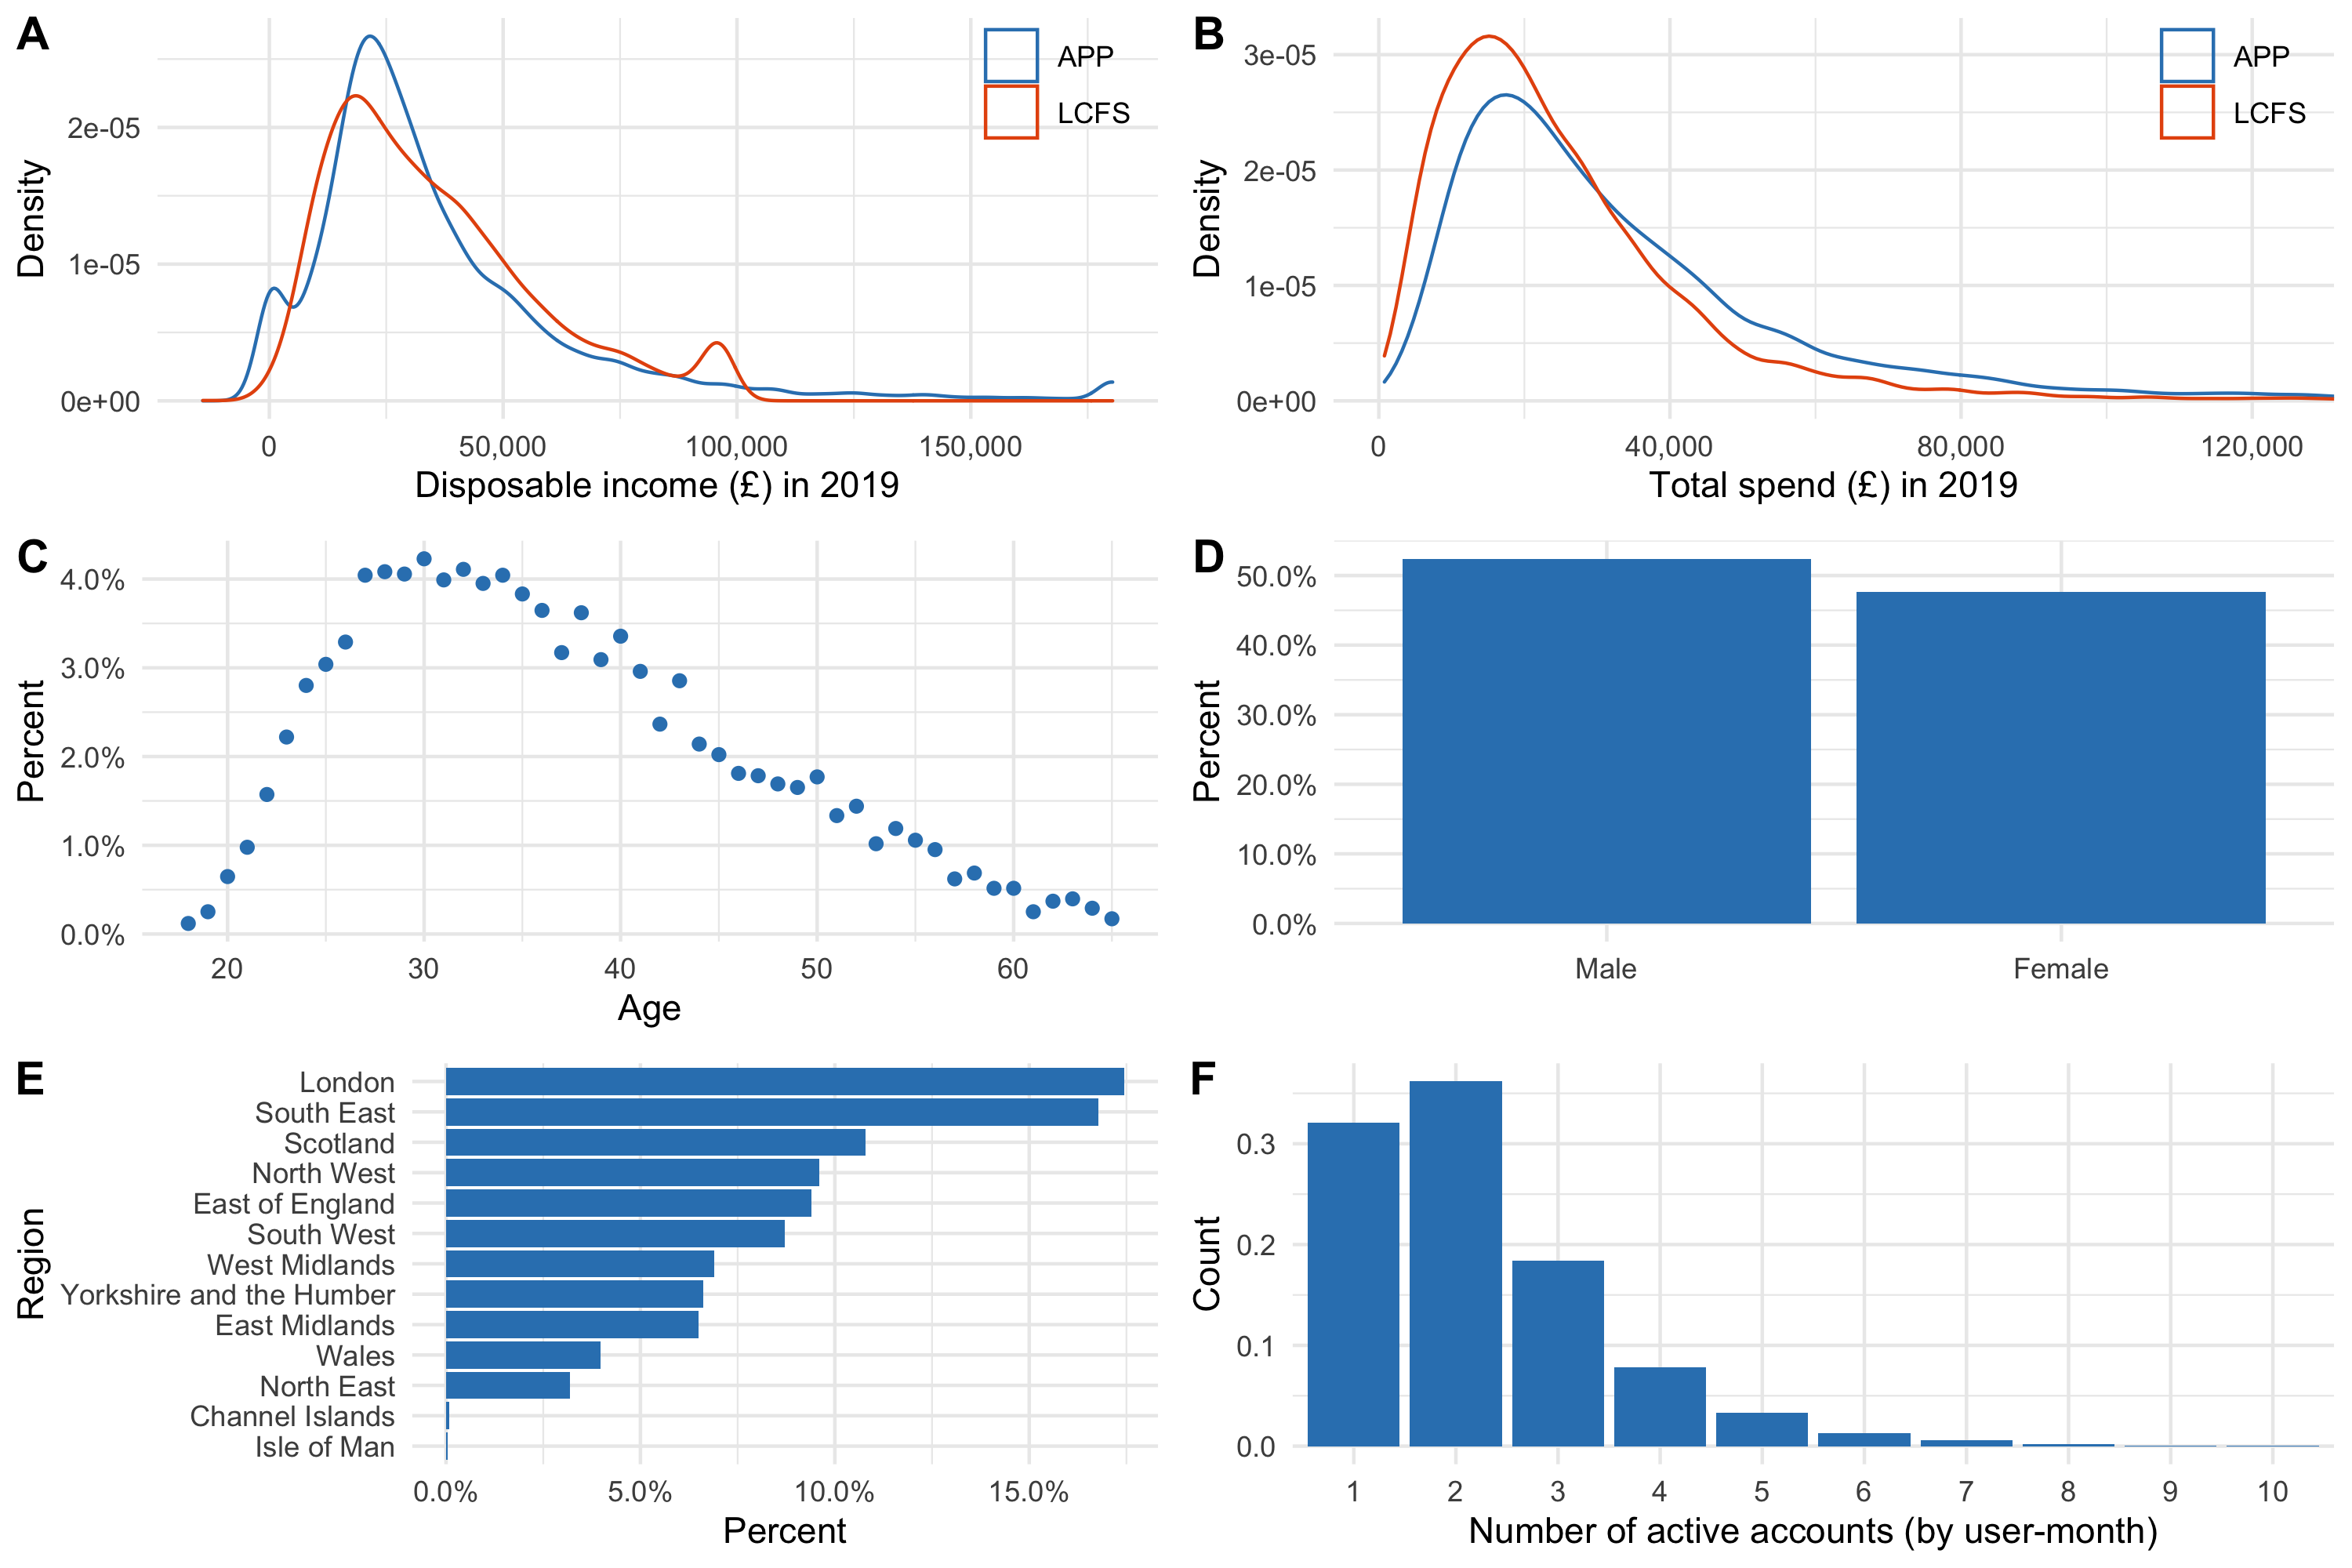
\includegraphics[width=\linewidth]{\figdir/sample_description.png}
    \label{fig:sample_description}
    \fignote{\textwidth}{Panels A and B show the distribution of disposable
        income and total spending in 2019, respectively, benchmarked against
        the 2018/19 wave of the ONS Living Cost and Food Survey (LCFS). The
        remaining panels show the data distributions of age, gender, region,
    and the number of active accounts.}%
\end{figure}

Table~\ref{tab:sumstats} provides summary statistics.


\begin{table}[htbp]
   \centering
   \tiny
   \begin{threeparttable}[b]
      \caption{\label{tab:reg_compare} Regression results}
      \begin{tabular}{lcccccc}
         \tabularnewline \midrule \midrule
         Dependent Variable: & \multicolumn{6}{c}{Net-inflows}\\
         Model:                     & (1)                   & (2)                & (3)                & (4)                & (5)               & (6)\\  
         \midrule
         \emph{Variables}\\
         App use                    & 14.330$^{**}$         & 15.303$^{***}$     & 15.303$^{***}$     & 19.381$^{***}$     & 15.963$^{**}$     & 20.207$^{***}$\\   
                                    & [2.650; 26.009]       & [3.686; 26.919]    & [3.686; 26.919]    & [7.110; 31.652]    & [1.881; 30.045]   & [7.940; 32.473]\\   
         Month income               &                       & 0.053$^{***}$      & 0.053$^{***}$      & 0.060$^{***}$      & 0.053$^{***}$     & 0.058$^{***}$\\   
                                    &                       & [0.049; 0.058]     & [0.049; 0.058]     & [0.045; 0.075]     & [0.045; 0.060]    & [0.043; 0.073]\\   
         Month spend                &                       & -0.077$^{***}$     & -0.077$^{***}$     & -0.100$^{***}$     & -0.076$^{***}$    & -0.098$^{***}$\\   
                                    &                       & [-0.081; -0.073]   & [-0.081; -0.073]   & [-0.109; -0.091]   & [-0.091; -0.061]  & [-0.107; -0.089]\\   
         Disc. spend                &                       & 138.940$^{***}$    & 138.940$^{***}$    & 169.002$^{***}$    & 132.862$^{***}$   & 156.441$^{***}$\\   
                                    &                       & [115.597; 162.282] & [115.597; 162.282] & [128.874; 209.129] & [90.975; 174.750] & [115.907; 196.976]\\   
         Female                     &                       & -14.521$^{***}$    & -14.521$^{***}$    &                    & -14.247$^{***}$   &   \\   
                                    &                       & [-24.998; -4.044]  & [-24.998; -4.044]  &                    & [-21.206; -7.289] &   \\   
         Generation $=$ GenX        &                       & 39.071$^{***}$     & 39.071$^{***}$     &                    & 39.379$^{**}$     &   \\   
                                    &                       & [19.258; 58.885]   & [19.258; 58.885]   &                    & [9.611; 69.148]   &   \\   
         Generation $=$ Millennials &                       & 71.330$^{***}$     & 71.330$^{***}$     &                    & 71.699$^{***}$    &   \\   
                                    &                       & [51.964; 90.697]   & [51.964; 90.697]   &                    & [40.338; 103.060] &   \\   
         Generation $=$ GenZ        &                       & 42.302             & 42.302             &                    & 43.095$^{*}$      &   \\   
                                    &                       & [-9.381; 93.985]   & [-9.381; 93.985]   &                    & [-7.002; 93.192]  &   \\   
         Intercept                  & -20.523$^{***}$       & -59.208$^{***}$    & -59.208$^{***}$    &                    &                   &   \\   
                                    & [-30.679; -10.368]    & [-84.179; -34.237] & [-84.179; -34.237] &                    &                   &   \\   
         \midrule
         \emph{Fixed-effects}\\
         User FE                    &                       &                    &                    & Yes                &                   & Yes\\  
         Month FE                   &                       &                    &                    &                    & Yes               & Yes\\  
         \midrule
         \emph{Fit statistics}\\
         Observations               & 184,847               & 184,847            & 184,847            & 184,847            & 184,847           & 184,847\\  
         R$^2$                      & $3.13\times 10^{-5}$  & 0.01132            & 0.01132            & 0.10137            & 0.01203           & 0.10203\\  
         Within R$^2$               &                       &                    &                    & 0.00905            & 0.01117           & 0.00885\\  
         \midrule \midrule
         \multicolumn{7}{l}{\emph{Signif. Codes: ***: 0.01, **: 0.05, *: 0.1}}\\
      \end{tabular}
   \end{threeparttable}
\end{table}




We use data from the 2018-2019 wave of the Office of National Statistics' Living Costs and Food
Survey (LCFS).\footnote{We accessed the data via the UK Data Service at the
following url:
\url{https://beta.ukdataservice.ac.uk/datacatalogue/studies/study?id=8686}.}
Data covers the period between April 2018 and March 2019.



\subsection{Treatment}%
\label{sub:treatment}

A user changes treatment status from untreated to treated when they start using
the app. Figure~\ref{fig:treatplot_sample_raw} shows the treatment history for
200 randomly selected users.

\begin{figure}[H]
    \centering
    \caption{Treatment assignment plot}%
    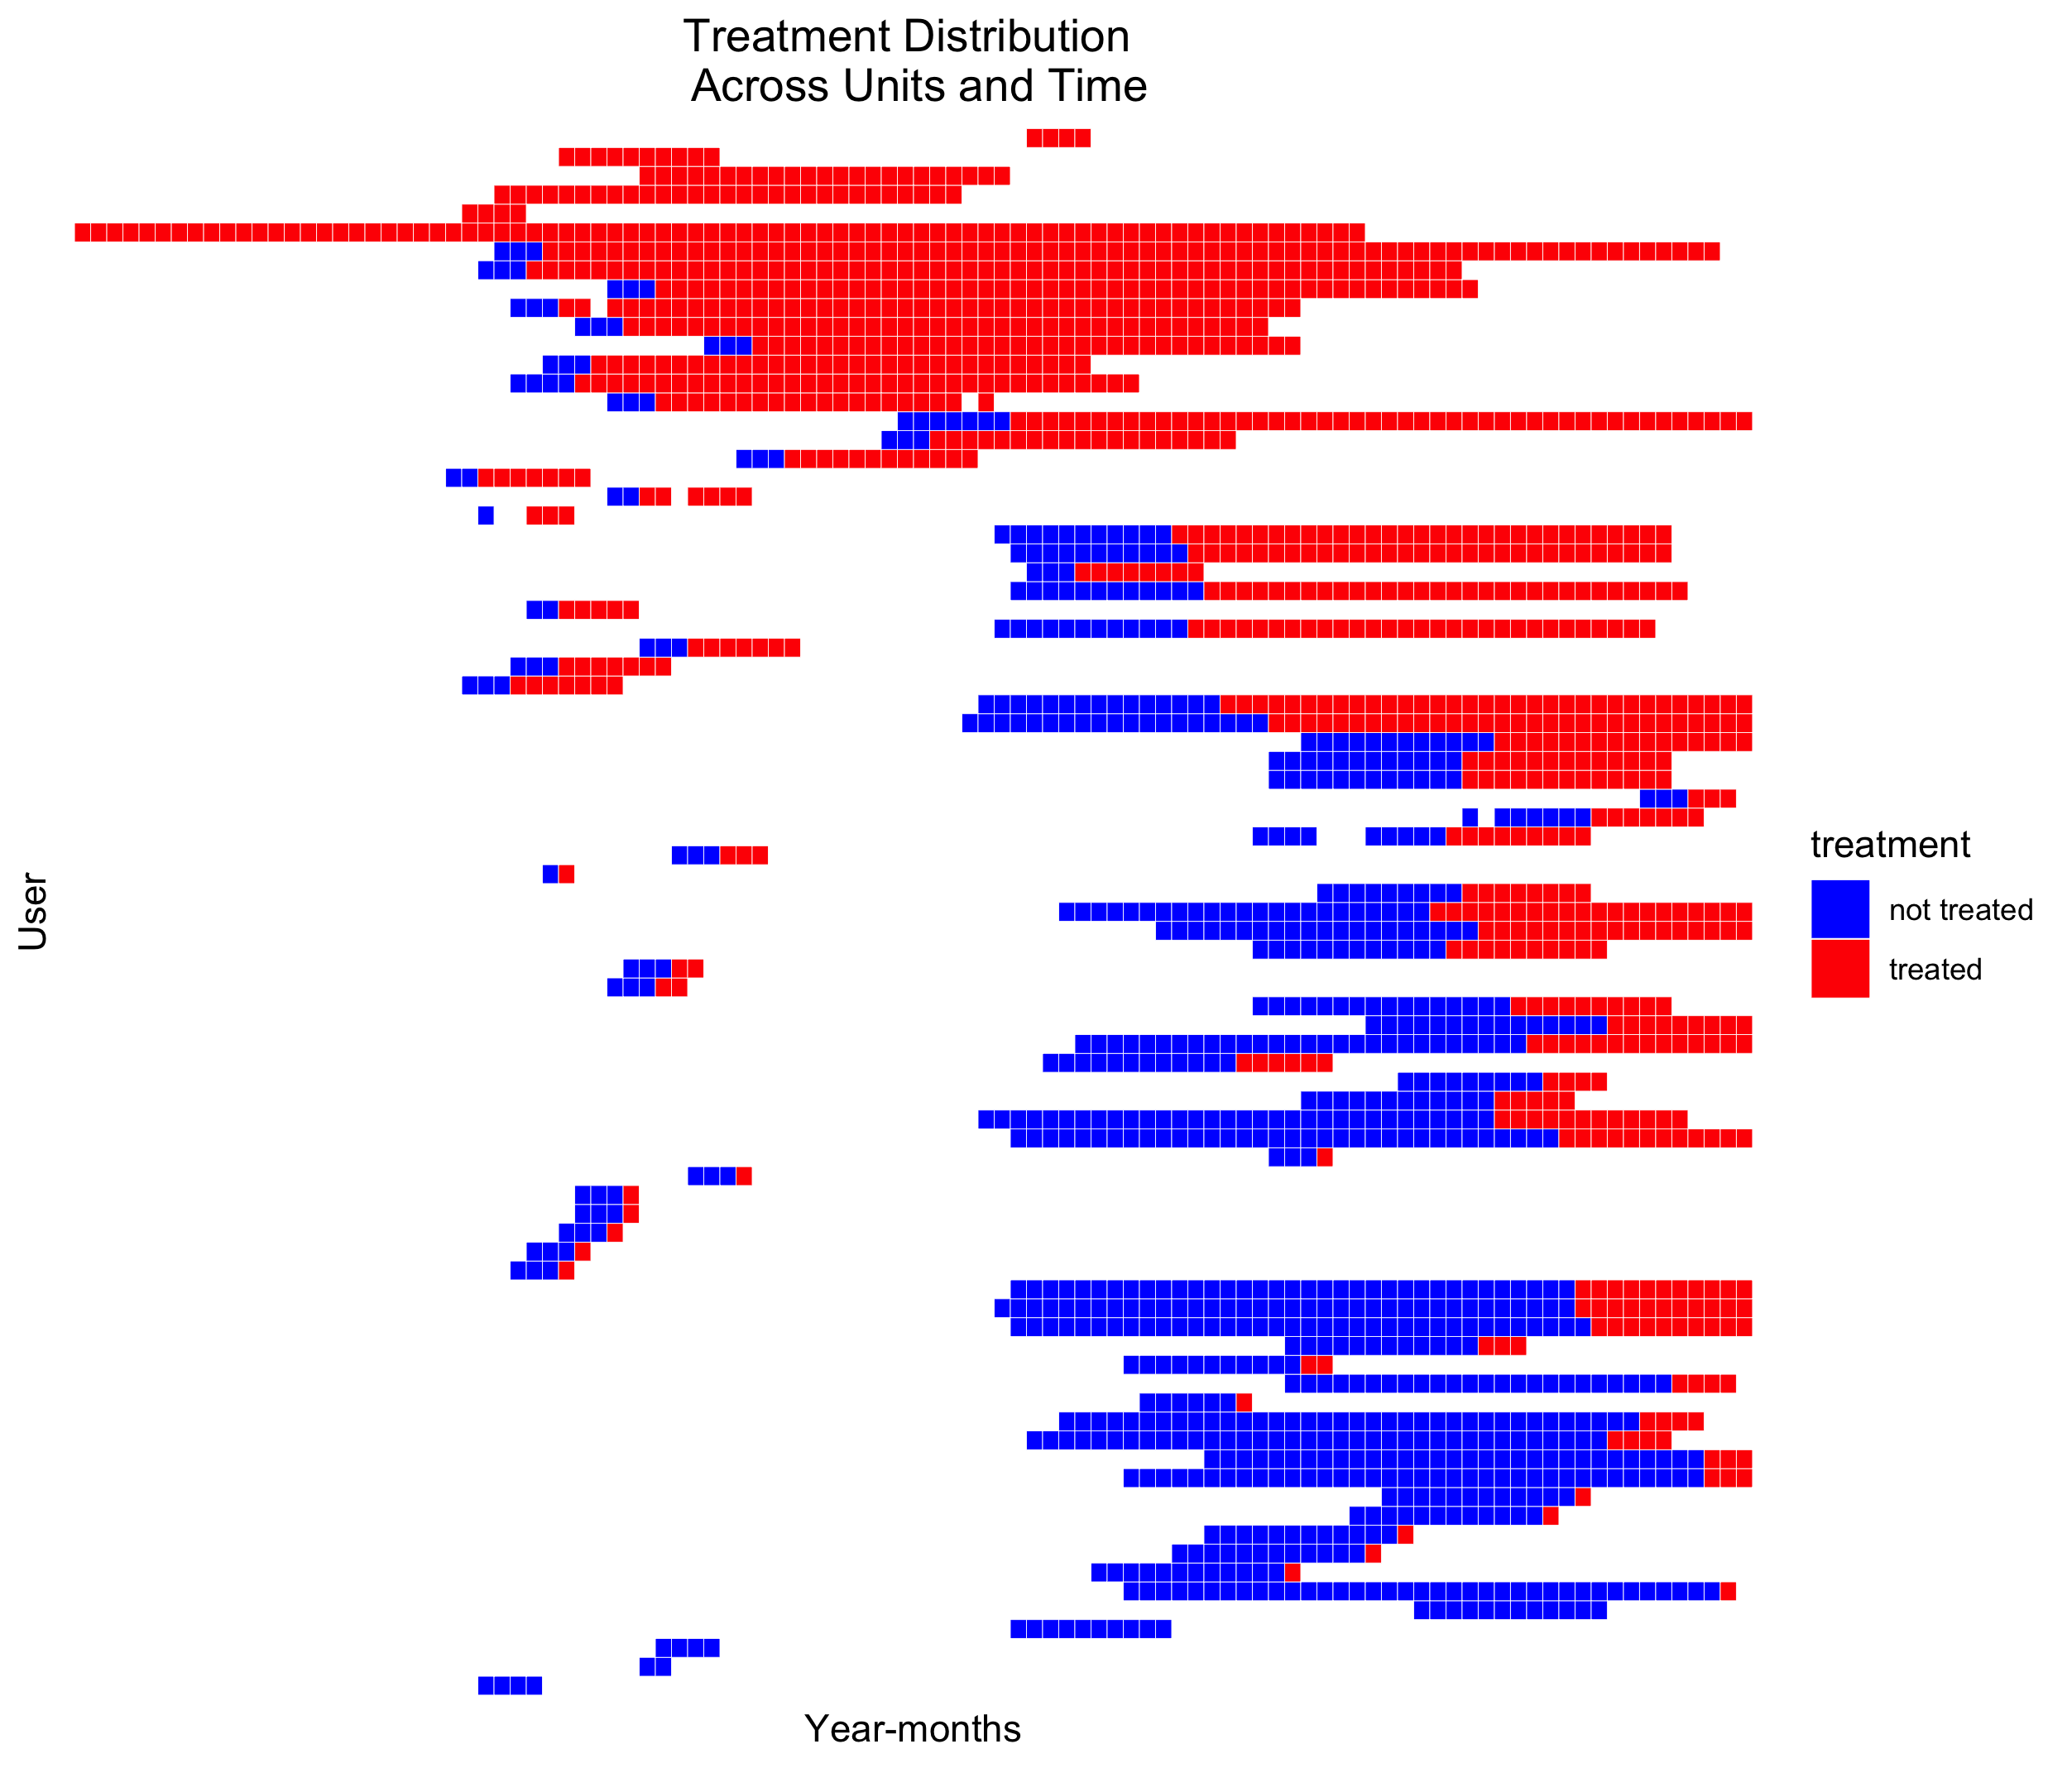
\includegraphics[width=0.8\linewidth]{\figdir/treatplot_sample_raw.png}
    \label{fig:treatplot_sample_raw}

    \fignote{\textwidth}{Each horizontal line shows the observed pre and post
        signup periods in blue and red, respectively, for one of 200 randomly
        selected users. The faint vertical white lines indicate month borders,
        whitespace indicates periods in which we do not observe the user. To
    the left of the observed period, this is because the app cannot access data
before that point when the user signs up; to the right, because they have
stopped using the app.}

\end{figure}


\subsection{Outcomes}%
\label{sub:outcomes}

Savings... see Table~\ref{tab:vars} for details.

For a more nuanced understanding of how app use affects savings we also
consider net-savings -- total savings account inflows minus outflows -- as a
proportion of monthly income to see whether a willingness to save more might be
offset by a (later) need to withdraw funds, and a dummy variable for whether a
user has any savings account inflows in a given month to see whether the app
helps users save at all. To investigate possible channels, we consider total
spend, highly discretionary spend, banking charges, the total amount of
borrowing, as well as payday borrowing, all as proportion of monthly income.



Net savings (\textit{netflows\_norm})
Inflows into minus outflows out of all of a user's savings accounts divided
by monthly income. To capture only ``user-generated'' flows, we exclude
interest and ``save the change'' transactions, as well as transactions of
less than \pounds5 in absolute
value. Monthly income and raw inflows and outflows are winsorised at the 1
percent level.
We focus on net inflows to capture effective savings.

Positive net savings dummy (\textit{has\_pos\_netflows})
Dummy equal to 1 if there were positive net savings (as defined above).
Captures extensive margin of savings (change in number of months with positive
net deposits)

Positive net savings (\textit{pos\_netflows})
Equal to net savings if there were positive net savings.
Captures intensive margin of savings (change in deposit amount in months with
positive net deposits)

\begin{figure}[H]
    \centering
    \caption{Savings patterns}%
    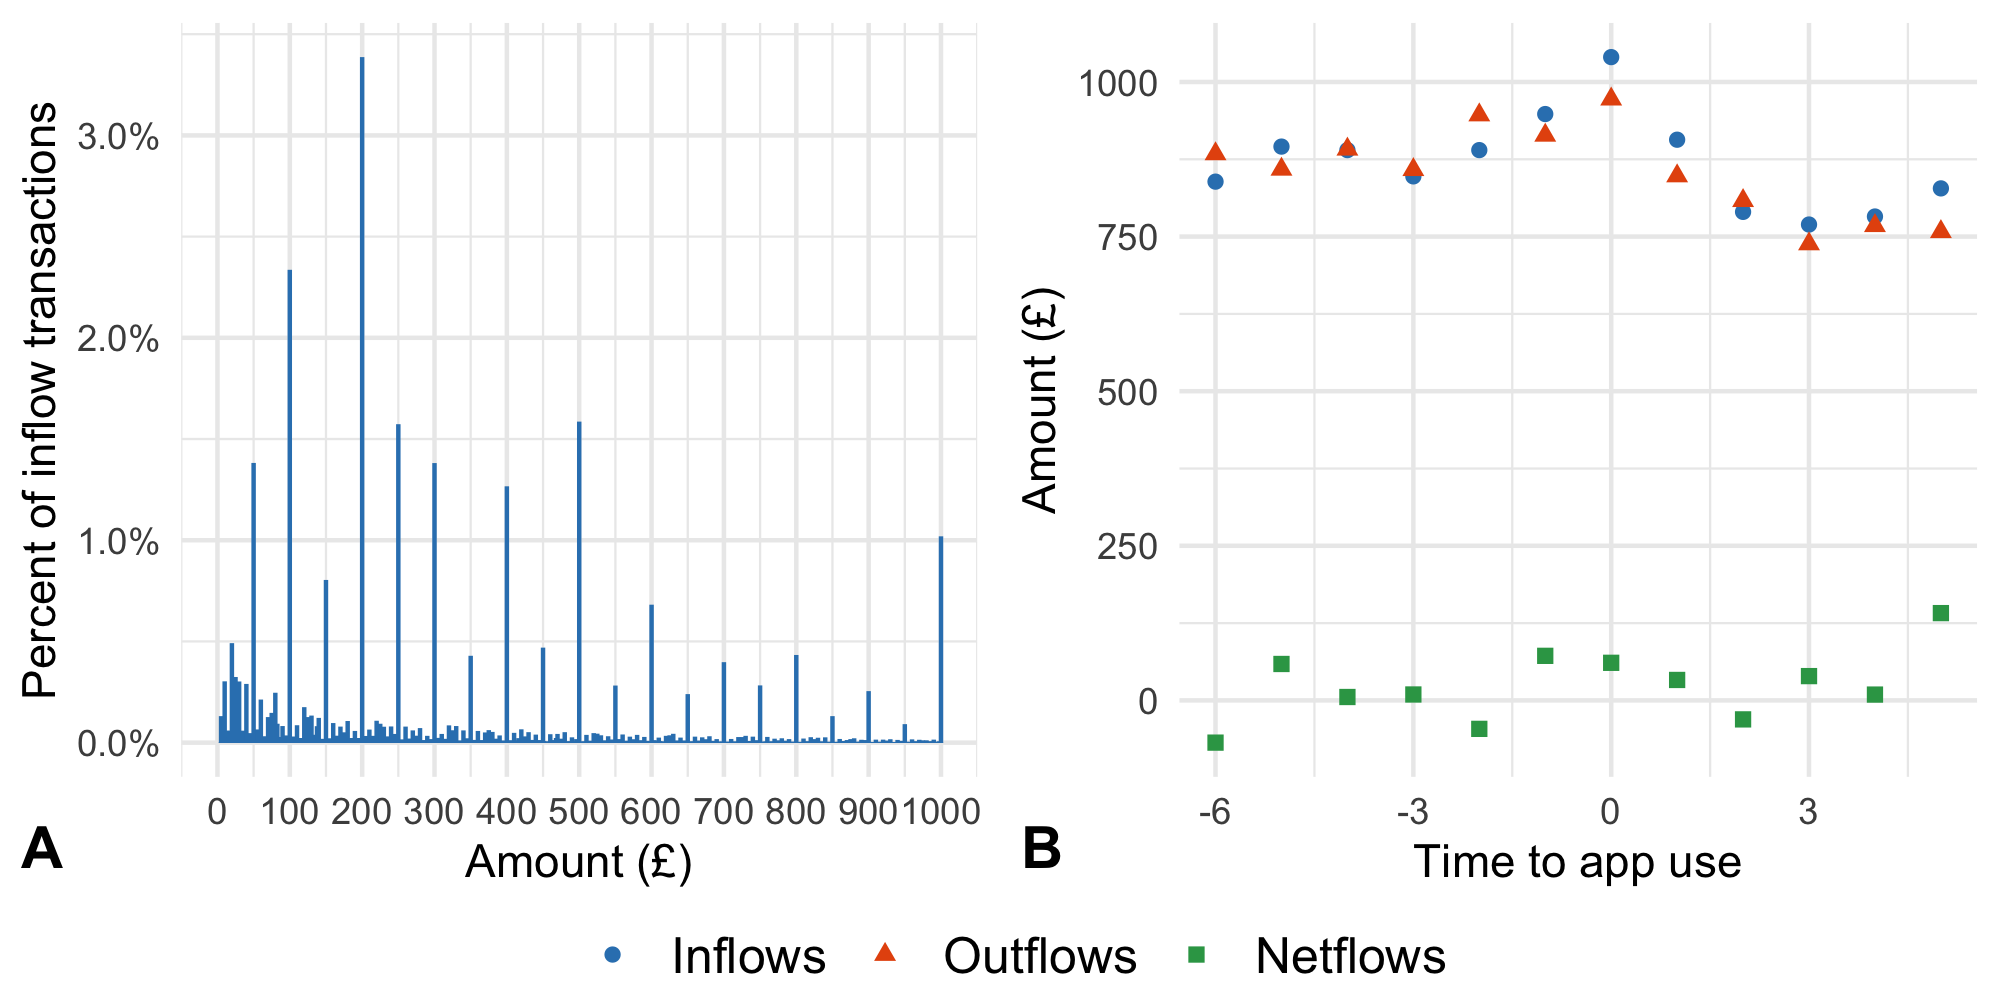
\includegraphics[width=\linewidth]{\figdir/savings_patterns.png}
    \label{fig:\figdir/savings_patterns}
    \fignote{\textwidth}{Panel A shows distribution of savings account inflow
        amounts, making clear that most transactions are the kinds of round
        amounts we would expect savings transactions to be. The data is
        truncated at \pounds1000. Panel B hows inflows, outflows, and netflows
        into savings accounts for six months before and five months after app
    use.}

\end{figure}


\paragraph{Adjusting for multiple hypothesis tests}%
\label{par:adjusting_for_multiple_hypothesis_tests}
We think of our secondary outcomes as exploratory and do not make any
adjustments for multiple hypothesis testing.\footnote{For a recent
game-theoretically motivated discussion of when and how to correct for multiple
hypothesis testing, see \citet{viviano2021should}.} An alternative approach,
based on \citet{anderson2008multiple}, would be to group outcomes into
``savings'', ``spending'', ``borrowing'', and ``fees'', and consider them as
different dimensions of a latent variable of interest which we might call
``financial management skills''. We do not do that for two reasons: first and
foremost, because we think it is natural to think of the amount saved as the
ultimate outcome and of other outcomes as providing a more nuanced
understanding of savings behaviour or as suggesting possible channels through
which app use affects savings. Thinking of savings as the main goal is also
reflected in Money Dashboard's main promise, which is to help users spend less
and save more, as shown in Figure~\ref{fig:mdb_website}. Second, as pointed out
in \citet{carlin2017fintech}, incurring overdraft fees is not an unambiguous
sign of a financial mistake, as the opportunity to go into overdraft confers a
benefit to the consumer.\footnote{For further discussions on fees, see
\citet{jorring2020financial, stango2009consumers}.}


\subsection{Covariates}%
\label{sub:covariates}

We control for baseline behaviour, events, and personal characteristics that,
to various degrees, capture a person's need, capacity, motivation, and
awareness to save. Table~\ref{tab:vars} lists all covariates used
together with their definition and the rationale for including them. For all
variables, we include contemporaneous values as well as lags for up to 6
periods. In addition, we control for the previous six months of savings to
capture time-invariant unobserved drivers of savings behaviour (in
specifications without fixed effects) as well as a possible signal for a higher
or lower need for future savings.

Following \citet{vanderweele2019principles} we include covariates that affect
either outcomes or the propensity for treatment or both, exclude from this
set of variables those that are instruments (affect the outcome only through their effect on
treatment propensity) and add to it proxies for unobserved variables that are a
common cause of both outcomes and treatment propensity.\footnote{
\citet{vanderweele2019principles} calls this the ``modified disjunctive cause
criterion'' for covariate selection, as it includes the set of variables that are causally
related to either outcomes, or treatment propensity, or both, but modified to
account for potential bias by excluding instruments and including proxies of
unobserved causes of both outcomes and treatment.}

The table below describes the construction and rationale for including of all
variables used. The code used to construct the variables is available on
\href{https://github.com/fabiangunzinger/mdb_eval/blob/d094f8cd364f64bbe3d4e644abbff726af86de2f/src/data/aggregators.py}{GitHub}.

\begin{table}[htpb]
    \centering\scriptsize
    \caption{Covariates}
    \label{tab:vars}
    \begin{tabularx}{\textwidth}{>{\raggedright\arraybackslash}X
        >{\raggedright\arraybackslash}X>{\raggedright\arraybackslash}X}
    \hline\hline
    Variable (name in dataset) & Definition  & Rationale \\
    \hline\\
    \multicolumn{3}{c}{\textbf{Primary outcome}}\\\\

    \multicolumn{3}{c}{\textbf{Covariates}}\\\\

    New loan dummy (\textit{new\_loan})&
    Dummy variable equal to 1 if user takes out a new loan. Calculated positive inflows
    of funds tagged as ``loan''.&
    Might increase (additional funds) or decrease (need to repay) propensity to
    save in month of takeout and lower propensity to save in the future due to
    need to repay.\\

    Unemployment benefits dummy (\textit{unemp\_benefits})&
    Dummy variable equal to 1 if user has inflow of funds tagged as ``job
    seeker benefits''.&
    Might lower a user's ability to save but increase their need for a money
    management app.\\

    Monthly income (\textit{month\_income})&
    Average monthly income in a calendar year, calculated as the sum of all
    credits tagged income payments in said year divided by 12.&
    Income may alter the need and ability to save and correlate with cognitive
    characteristics that alter a person's propensity to use a money management
    app.\\

    \hline\hline
    \end{tabularx}
\end{table}




\subsection{Estimation}%
\label{sub:difference_in_difference}

We choose a window from -6 to 5 for two reasons: because the longer a window we
consider, the less plausible our ceteris paribus assumption is, and the longer
the window, the smaller our sample.


\subsection{Code access}%
\label{sub:code_access}

We provide links to code that creates key elements of the paper such as
variable definitions and sample selection directly in the relevant places in
the paper so they can be accessed conveniently. The links are indicated with
the GitHub logo, \faGithub. The hope is that this helps the
curious reader clarify questions about subtleties they might have while reading
the paper. The complete projects GitHub repo is at
\href{https://github.com/fabiangunzinger/mdb\_eval}{https://github.com/fabiangunzinger/mdb\_eval}.



\section{Methods}%
\label{sec:data}

While we were unable to pre-register the analysis because we have had access to
and been working with the Money Dashoard data for months, we proceeded in the
same spirit: we first wrote a draft of the paper in the form of a pre-analysis
plan, following \citet{olken2015promises}, then tested the entire code base --
data pre-processing, balance checks, main analysis, and extensions -- with a 1
percent sample, and finally ran the entire analysis.


\subsection{Dataset}%
\label{sub:dataset}


\subsection{Sample selection}%
\label{sub:sample_selection}

To assess the impact of MDB use on users' financial behaviour we need to
observe their relevant financial history for a sufficiently long period of time
prior to and after they started using the app. For our purpose here, ``relevant
financial history'' includes the complete set of spending transactions and all
savings account inflows and outflows, and ``sufficiently long period'' is a
period of 6 months prior to and after signup, with the month of signup being
the first month of the latter period.\footnote{In
Appendix~\ref{sub:alternative_matching_method} we show results with different
window lengths. \edit{The results are unchanged.}}

Table X provides an overview of the precise conditions we applied to implement
these criteria and their effect on the sample size. The set of functions that
implement each condition can be found on \href{path-to-github}{path to github}.


\subsection{Treatment}%
\label{sub:treatment}

Provide information about signup patterns


\subsection{Outcomes}%
\label{sub:outcomes}

\paragraph{Primary outcome}%
\label{par:primary_outcome}

Our main outcome variable is savings as a proportion of monthly income, where
we measure savings as the sum of all savings account inflows.


\paragraph{Secondary outcomes}%
\label{par:secondary_outcomes}

For a more nuanced understanding of how app use affects savings we also
consider net-savings -- total savings account inflows minus outflows -- as a
proportion of monthly income to see whether a willingness to save more might be
offset by a (later) need to withdraw funds, and a dummy variable for whether a
user has any savings account inflows in a given month to see whether the app
helps users save at all. To investigate possible channels, we consider total
spend, highly discretionary spend, banking charges, the total amount of
borrowing, as well as payday borrowing, all as proportion of monthly income. We
think of these additional outcomes as exploratory and do not make any
adjustments for multiple hypothesis testing.\footnote{For a recent
game-theoretically motivated discussion of when and how to correct for multiple
hypothesis testing, see \citet{viviano2021should}.}

An alternative approach, based on \citet{anderson2008multiple}, would be to
group outcomes into ``savings'', ``spending'', ``borrowing'', and ``fees'', and
consider them as different dimensions of a latent variable of interest which we
might call ``financial management skills''. We do not do that for two reasons:
first and foremost, because we think it is natural to think of the amount saved
as the ultimate outcome and of other outcomes as providing a more nuanced
understanding of savings behaviour or as suggesting possible channels through
which app use affects savings. Thinking of savings as the main goal is also
reflected in Money Dashboard's main promise, which is to help users spend less
and save more, as shown in Figure~\ref{fig:mdb_website}. Second, as pointed out
in \citet{carlin2017fintech}, incurring overdraft fees is not an unambiguous
sign of a financial mistake, as the opportunity to go into overdraft confers a
benefit to the consumer.\footnote{For further discussions on fees, see
\citet{jorring2020financial, stango2009consumers}.}

\subsection{Covariates}%
\label{sub:covariates}

Description of covariates.


\subsection{Difference-in-difference}%
\label{sub:difference_in_difference}

Control group design:
\begin{itemize}

    \item We only have data for a self-selected group of people who choose to
        use Money Dashboard. By virtue of signing up to an app that helps them
        manage their money, these users are different from those who don't sign
        up. As a result, we are unable to answer the question of whether use of
        Money Dashboard helps the average person in the population as a whole
        save more.\footnote{One way to get closer to that answer is to
            re-weight our sample on observable demographic variables so as to
            match the UK population as a whole. But our sample differs from the
            population as a whole both is ways that are observable (demographic
            variables) and unobservable (self-awareness that they need help
            managing their money, cognitive resources to engage with the app,
            motivation to do so). Re-weighting would only help us deal with the
        first of these.} Instead, we are answering the question whether Money
        Dashboard succeeds in helping its \textit{users} save more.

    \item Money Dashboard can access up to three years of historic data for
        each account a user links to their account.

    \item Each user for whom we have sufficient data thus serves as both a
        treatment unit and a potential control unit.

    \item We use a difference-in-differences design to estimate the effect of
        app use. Because we do not have a separate control group, we use the
        per-signup data of Money Dashboard users as control periods and use
        matching to find comparable control user for each tretment user.

    \item To perform the matching, we proceed as follows:

    \item Selection of covariates: all variables that simultaneously affect
        treatment and outcomes. No need to control for fixed effects: these
        capture unobserved time-invariant factors that make an individual sign
        up to MDB and affect its spending habits. Given that these are time
        invariant, and that all users eventually sign up, there is no
        difference between control and treatment units in these factors. Month
        of year: should probably include, as can affect p of signup and
        spending behaviour.

    \item For treatment units, we select data for six months before and after
        signup, where the month of the signup is treated as the first of the
        six after-signup months. For each user, we then calculate the mean
        value of each covariate for the pre-signup period.

    \item We construct potential control units as all 12-month data windows we
        observe before signup, and for each potential control unit calculate
        the mean value of each covariate for the first six months.


    \item Calculate propensity scores and eliminate obs outside common support?


    \item We use matching proceedure introduced in \citet{ho2007matching} and
        implemented in the \textit{MatchIt} R-package \citep{stuart2011matchit} to
        find most similar comparison unit for each treatment unit.

    \item Choice of exact matching proceedure:

        \begin{itemize}

            \item \edit{Matching with or without replacement? I'd think with,
                but read papers and check vignettes for trade-offs.}
                \citet{ho2007matching}: if many more good (with common support)
                control than treatment units available, use many to one
                matching, else do matching with replacement. Check for common
                support using convex hull analysis from
                \citet{king2006dangers}.

            \item Match more exactly on variables that are more correlated with
                outcome. How to determine? Correlation? Cutoff for "high"
                correlation?

            \item We start with exact matching (matching all possible control
                units that exactly match the treatment unit). For continuous
                variables, we use 6 buckets (default in
                \citet{stuart2011matchit}).

            \item If we match more than X percent of treatment observations, we
                stop. If not, we move to another approach. The goal of
                proceedure is to avoid biased estimates due to the deletion of
                too many treatment units \citep{rosenbaum1985bias}.

            \item We use nearest-neighbour matching based on propensity score.
                If we succeed in balancing covariates, we stop. If we don't we
                use more sophisticated specifications to estimate the
                propensity score. See \citet{ho2007matching} section 6.4.

            \item We asses balance following
                \href{https://kosukeimai.github.io/MatchIt/articles/assessing-balance.html}{vignette}.

            \item Check for reduction in moden dependence producing equivalent
                of Fig. 2 in \citet{ho2007matching}.

        \end{itemize}
\end{itemize}


Open questions:
\begin{itemize}
    \item Do we include fixed effects after matching? Reason not to: we use the
        same units for treatment and control, so time-invariant unobserved
        differences should be equally distributed across treatment and control.

    \item How does event studies in \citet{sun2021estimating} relate to all
        this? Is key difference that event studies use periods since treatment
        rather than time?

\end{itemize}


% Estimation equation for static comparison:
% \begin{equation}
%     y_{it} = \alpha + 
% \end{equation}

Estimating treatment effects
\begin{itemize}

    \item Our estimate is the ATT, not the ATE. 

    \item First, we present pre and post signup comparisons without matching
        (i.e. control group is user pre-signup).

    \item Second, we present (static) pre-post using matched comparisons.

    \item Third, we present dynamic pre-post using matched comparisons. Need to
        think about how this relates to \citet{sun2021estimating}, who propose
        an unbiased estimator for dynamic two-way FE event study designs. I
        think our analysis nests theirs, since we might still want to include
        fixed and time effects, though I need to think about this. (Reason to
        do so: we won't be able to match perfectly, so including user and time
        fixed effects to control for unit and time invariant variation still
        seems useful).

    \item As alternative to matching, consider synthetic controls for
        disaggregated data \citep{abadie2021penalized}.

\end{itemize}

Is estimate causal?
\begin{itemize}
    \item \citet{king2006dangers} show that there are four sources of bias
        (ommitted variable, posttreatment, interpolation, extrapolation).
    
    \item Discuss each in turn to argue that effect is causal (for our population
        of interest, which are people signing up to MDB). 
\end{itemize}


% % !TEX root = ../eval.tex

\section{Results}%
\label{sec:results}


\subsection{Dynamic TWFE}%
\label{sub:dynamic_results}

\begin{equation}
\label{eq:dynamic_twfe}
    y_{it} = \sum^{5}_{s=-6} \beta_s D_{it}^s + \alpha_i + \lambda_t + \gamma X_{it} + \epsilon_{it},
\end{equation}

where $y_{it}$ is the outcome for individual $i$ at time $t$, $\alpha_i$ and
$\lambda_t$ are individual and year-month fixed effects, respectively, and
$X_{it}$ is a vector of individual and time varying controls. $D_{it}^s$ equals
1 if, in period $t$, individual $i$ is $s$ months away from signing up to the
app. The set of $\beta_s$ coefficients measure the effect of treatment $s$
periods away from treatment, which is what we are interested in.

To avoid multicollinearity issues and uniquely identify the lead and lag
effects, we omit relative period indicator $s = -1$, and bin the endpoints of our
observation window so that $D_{it}^{-6} = 1$ for all periods six or more
periods prior to signup and $D_{it}^{5} = 1$ for all months five or more months
after the month of signup. This expresses all estimates relative to the omitted
period, which -- given that it is the last month before signup -- serves as a
natural benchmark. Binning endpoints assumes that coefficients remain constant
outside the observation window. Both of these approaches are standard in the
literature, as discussed in \citet{sun2021estimating, schmidheiny2019event}.

% We omit the relative period indicator for period $s = -1$ because we need to
% omit one relative period indicator to avoid perfect collinearity among the
% period indicators, and we choose the last pre-treatment period because it
% serves as a natural benchmark against which to compare the outcomes in other
% periods.\footnote{As \citet{sun2021estimating} point out, there are two sources
% of perfect multicollinearity when estimating a fully dynamic model (i.e. one
% including all possible lags). The first results from all relative period
% indicators summing to 1 in each period, so that the entire set of relative period
% dummies across all time periods is perfectly multicollinear. We deal with this
% by excluding the indicator for $s = -1$. The second issue arises from the fact
% that for initial treatment period $E_i$, $t = s + E_i$. We deal with this issue
% by "trimming" our sample to be balanced in relative periods by only using
% data from relative periodl $\{-6, 5\}$. Both of these approaches are standard
% in the empirical literature.}

\begin{figure}[H]
    \centering
    \caption{Main results}%
    \label{fig:dspend_main}
    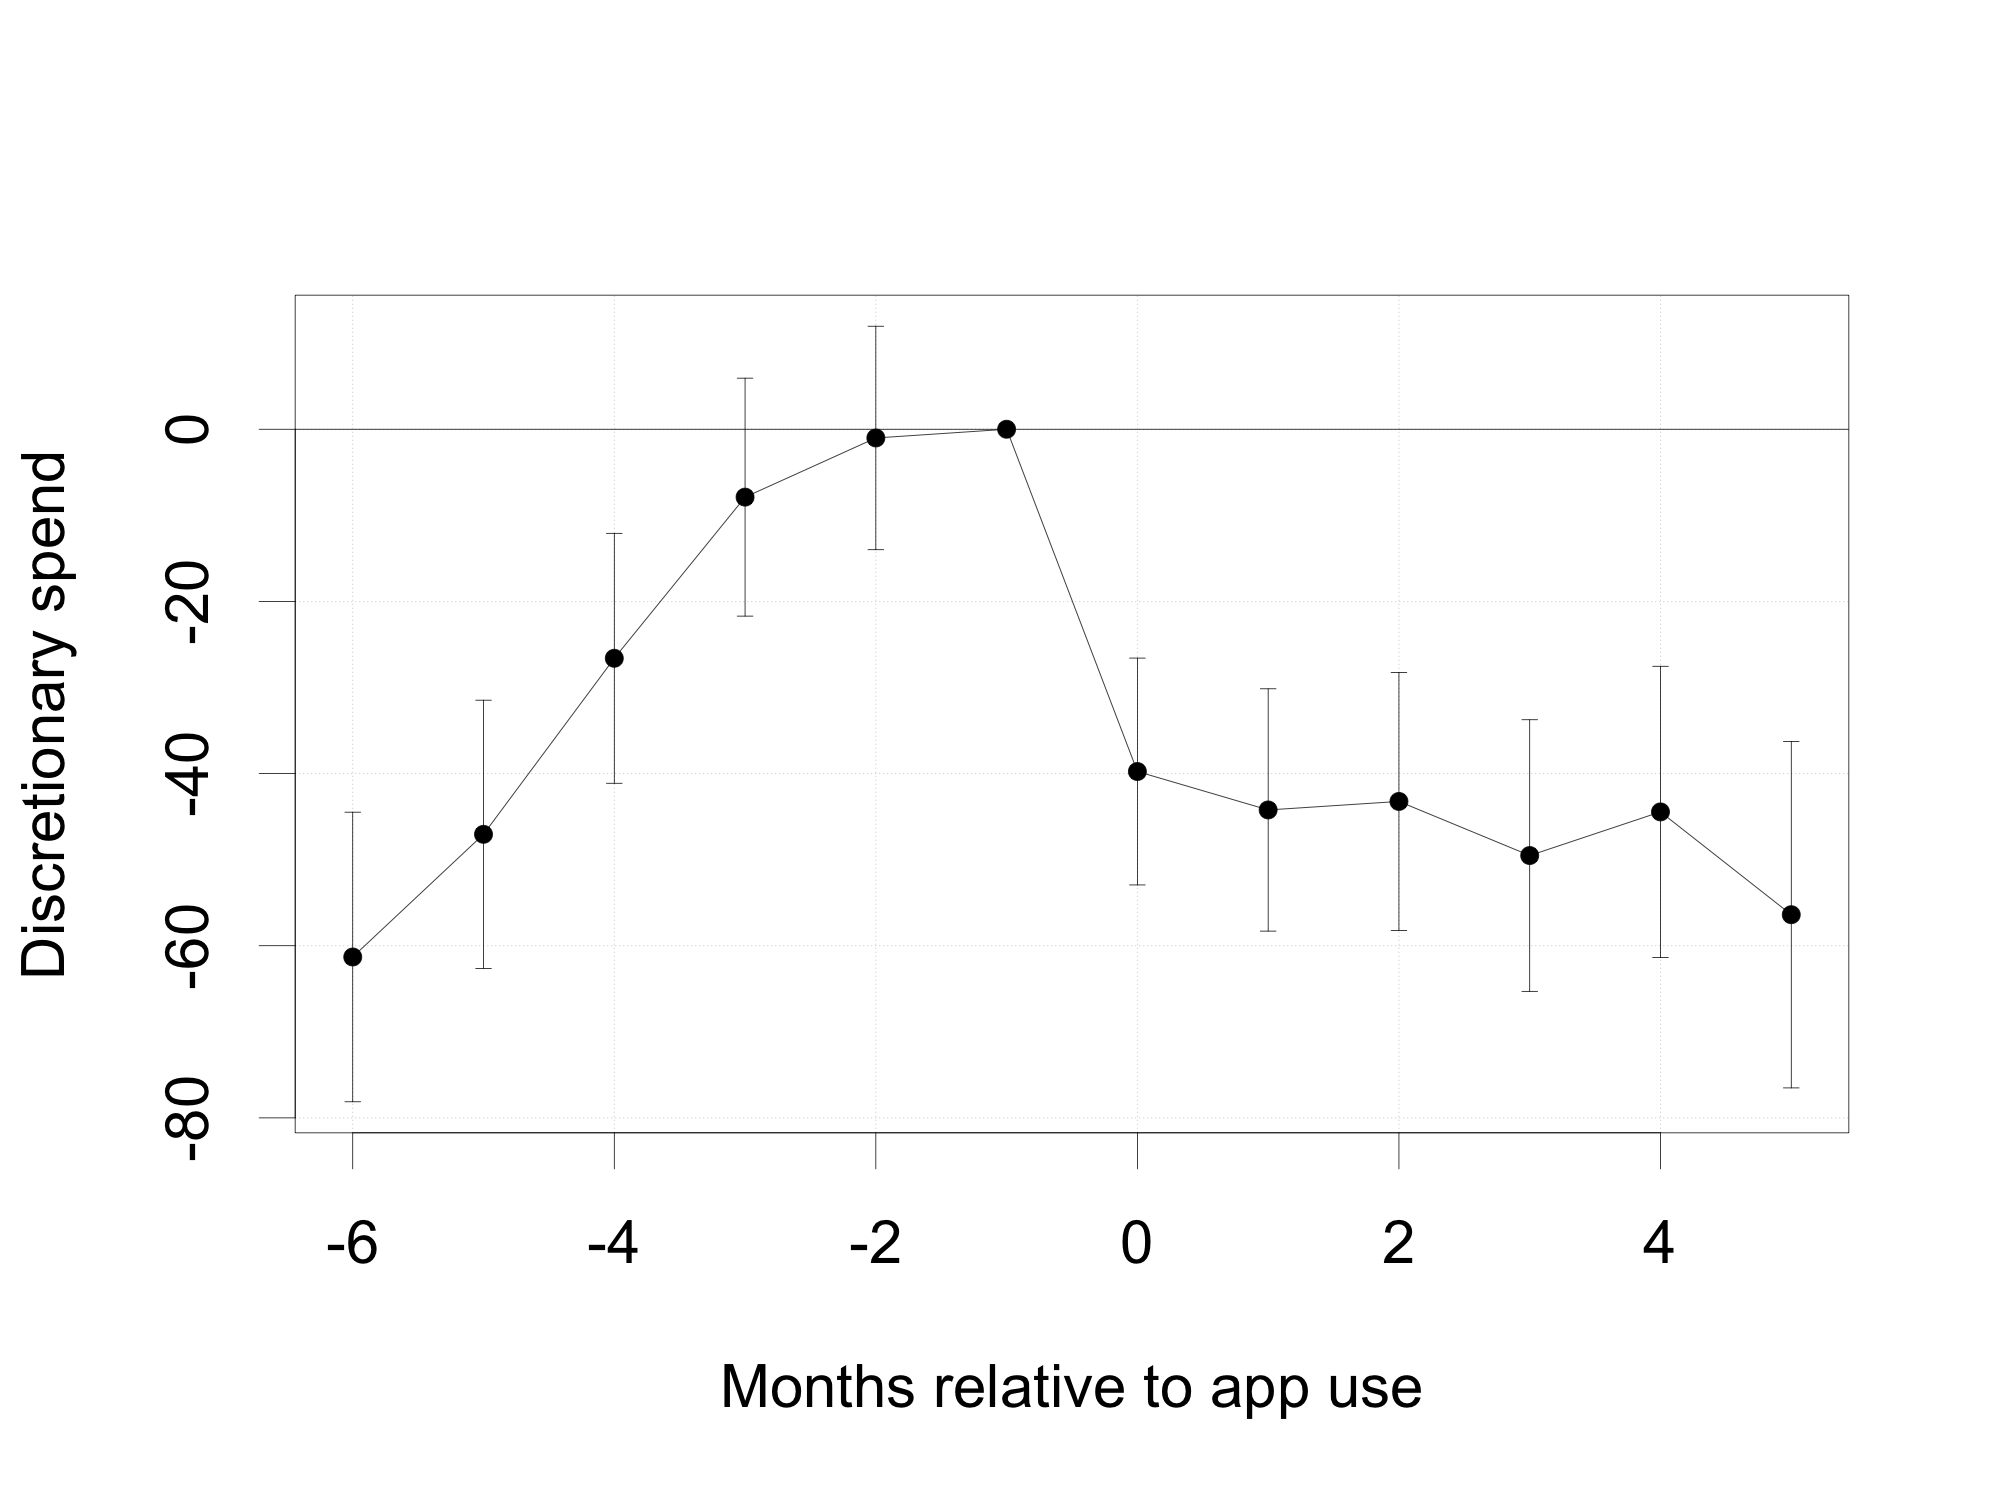
\includegraphics[width=.49\textwidth]{\figdir/dspend_main.png}
    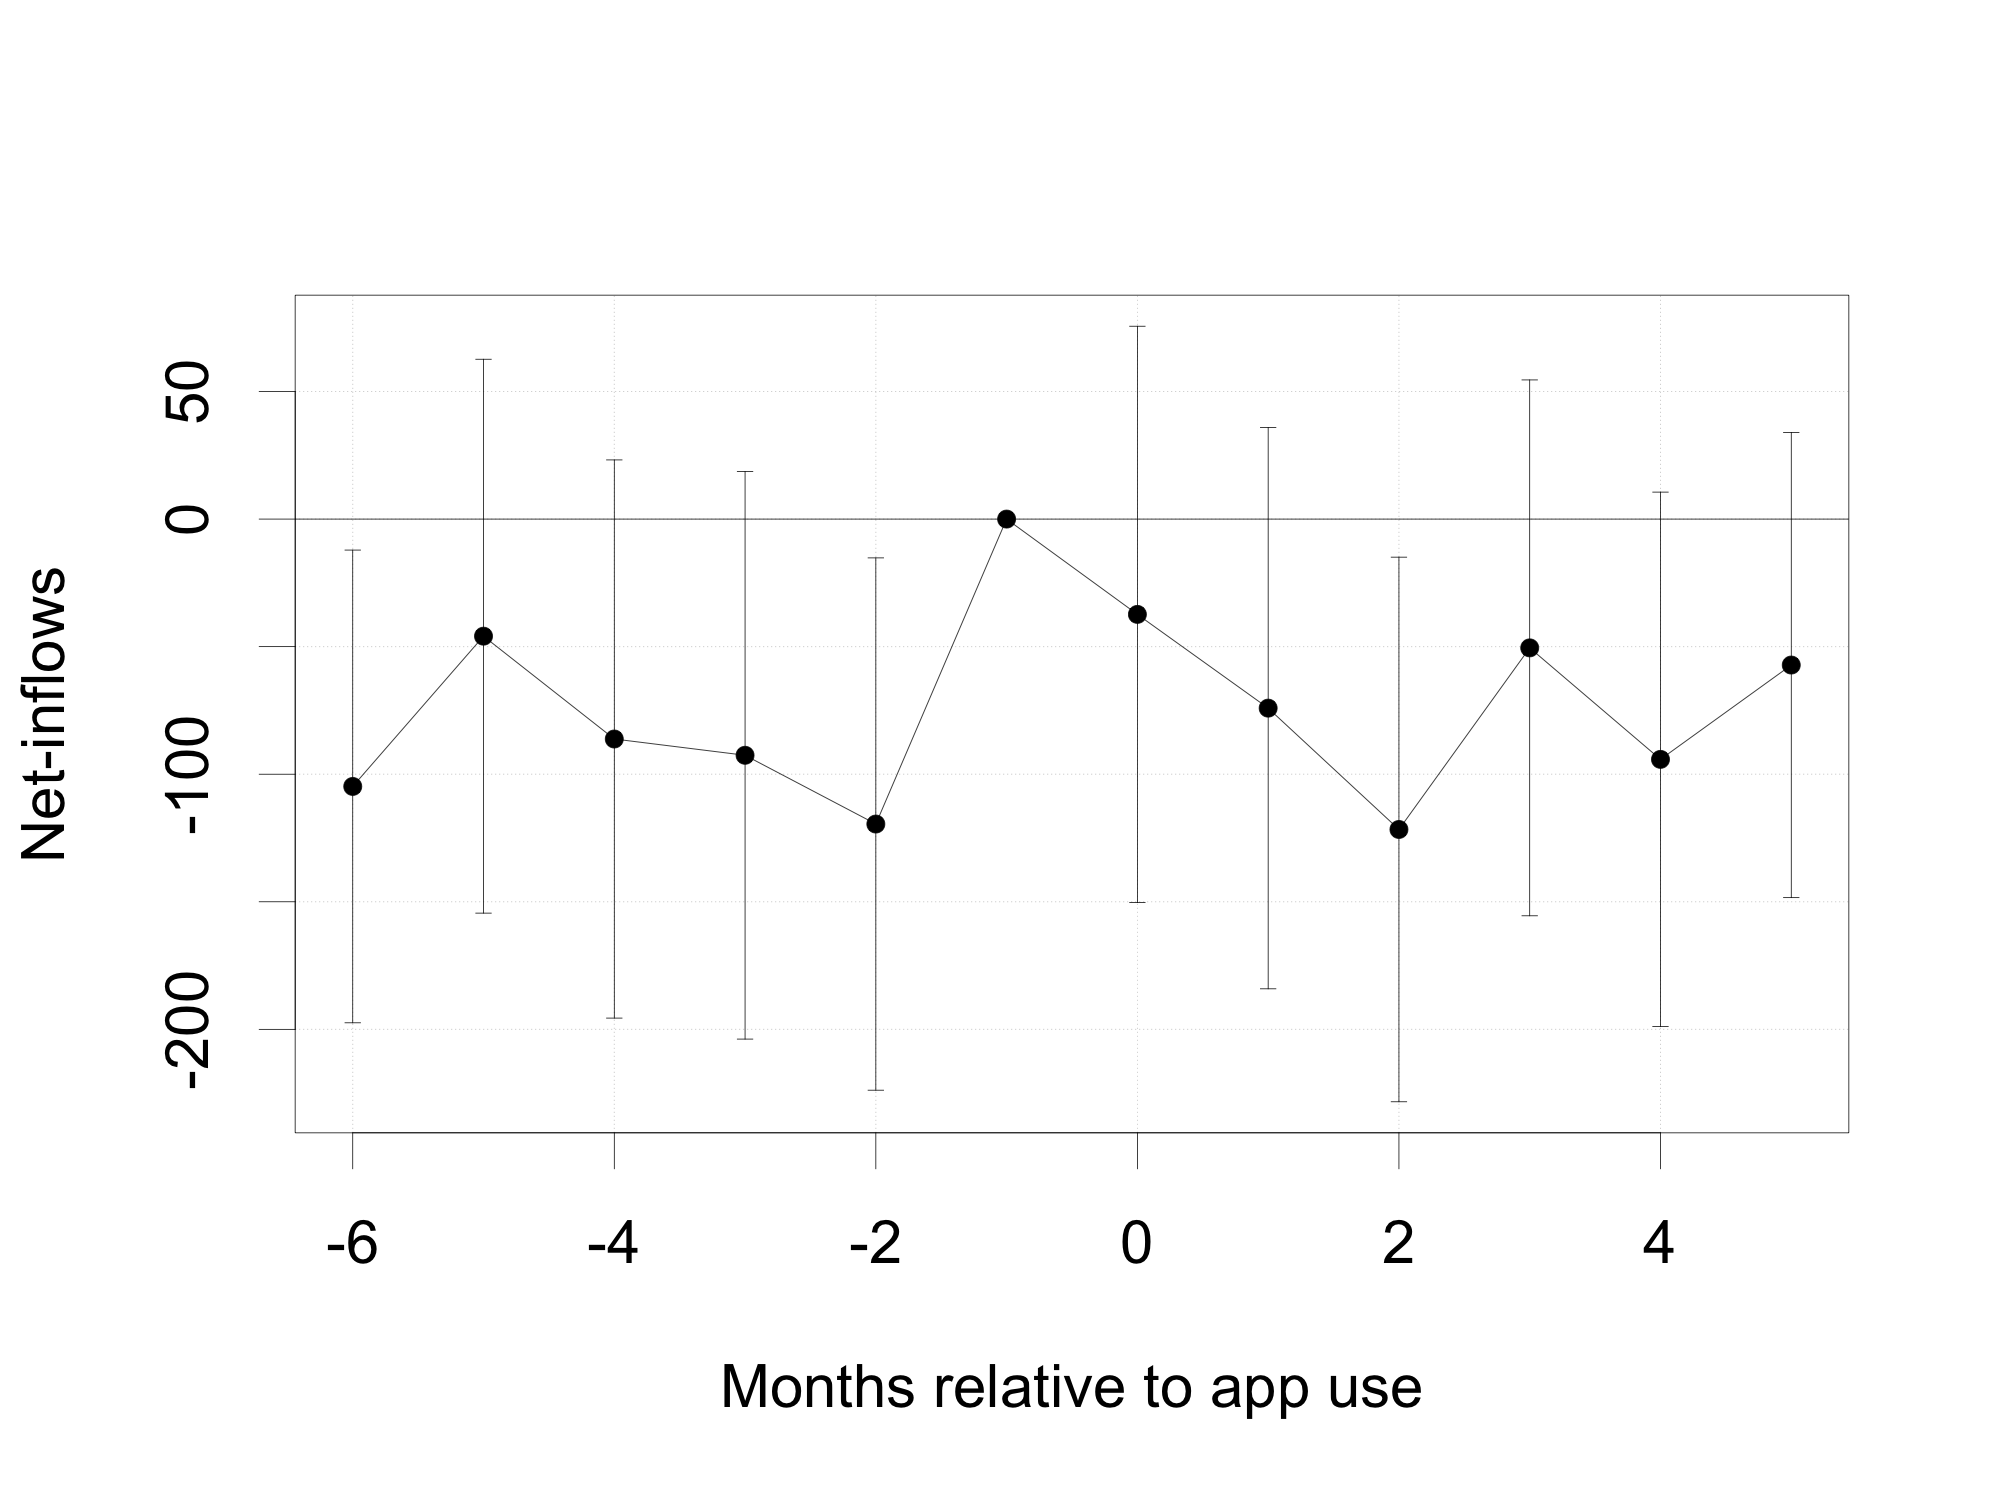
\includegraphics[width=.49\textwidth]{\figdir/netflows_main.png}
    \fignote{\textwidth}{Figures show estimates of leads and lags frome
        estimating model~(\ref{eq:dynamic_twfe}) with distretionary spend (left) and
netflows into savings accounts (right) as the dependent variable. Standard
errors are clustered by user.}
\end{figure}





% \citet{sun2021estimating} define an event study design as a staggered adoption
% design where units are treated at different times and where there may or may
% not be never treated units. In our case, we have no never treated units, and
% treatment is absorbing in that once a unit is treated they will also be treated
% in all subsequent units.\footnote{We cannot rule out that some users who
% stopped using the app and closed their account rejoined later on, in which case
% they would appear in our dataset as a new user. However, we can plausibly
% assume that such cases are rare.} 

% Setup:
% \begin{itemize}
%     \item We observe $N+1$ unites for $T+1$ periods and, for each
%         $i\in\{0,\ldots, N\}$ and $t\in\{0,\ldots,T\}$ observe outcome $y_{it}$
%         and treatment status $D_{it}\in\{0, 1\}$, where $D_{it}$ equals 1 if unit
%         $i$ is treated in period $t$ and 0 otherwise.

%     \item We can uniquely characterise treatment paths by the time period of
%         initial treatment, denoted as $E_i = min\{t: D_{it} = 1\}$.

%     \item We can group units into cohorts $e \in \{0,\ldots, T\}$, where units
%         in cohort $e$ were all first treated at time $e$, so that $\{i: E_i =
%         e\}$.

%     \item We define $y^e_{it}$ as the potential outcome in period $t$ if unit
%         $i$ was first treated in period $e$.

% \end{itemize}


% Assumptions:
% \begin{itemize}
%     \item Observations $\{y_{it}, D_{it}\}_{t=0}^T$ are independent.

%     \item A1: parallel trends: difference in baseline outcomes over time do
%         not differ between treatment cohorts. Not obviously violated in our
%         context. Early adopters might differ from late adopters, but difference
%         might plausibly be constant over time. - We don't have never treated
%         units, so Ashenfelter dip scenario is not a problem, even though we
%         seem to observe something like this in discretionary spending graph
%         (increase in disc spend before signup)

%     \item A2: no anticipatory behaviour. Plausibly violated if people are
%         motivated to save more and start doing so even before app use. Can test
%         for whether there is a peak prior to signup. Because our units have
%         private knowledge about future of treatment path (their intention to
%         reduce spending and save more and sign up to an app), this might be
%         violated. The trajectories of discret spend and net inflows are
%         conflicting on this, though, suggesting that they increases discret
%         spend in runup to app use (which might provide motivation to eventually
%         sign up) but also might have increased net savings slightly.

%     \item A3: treatment effect homogeneity across all cohorts and all relative
%         periods. (Note: treatment effects can be dynamic, but need to be the
%         same across cohorts). We could test for this.

% \end{itemize}


% Notes:
% \begin{itemize}

%     \item Comparison: pre vs post signup within each individual.

%     \item Assumption: there are no time-varying unobserved effects that affect
%         both y and D (formally: $E[Du] = 0$, since u is by definition
%         correlated with y.

%     \item Discussion: there is something that made the individual sign up in
%         the first place, and it might well be an individual level shock that we
%         don't observe (unexpected large expense, loss of job, exposure to
%         something that motivates saving or change in financial behaviour).

%     \item See \citet{imai2021use} for problems with twfe

% \end{itemize}



\subsection{Decomposing intensive and extensive margins}%
\label{sub:decomposing_intensive_and_extensive_margins}

\begin{figure}[H]
    \centering
    \caption{Decomposition of intensive and extensive margins}%
    \label{fig:intext}
    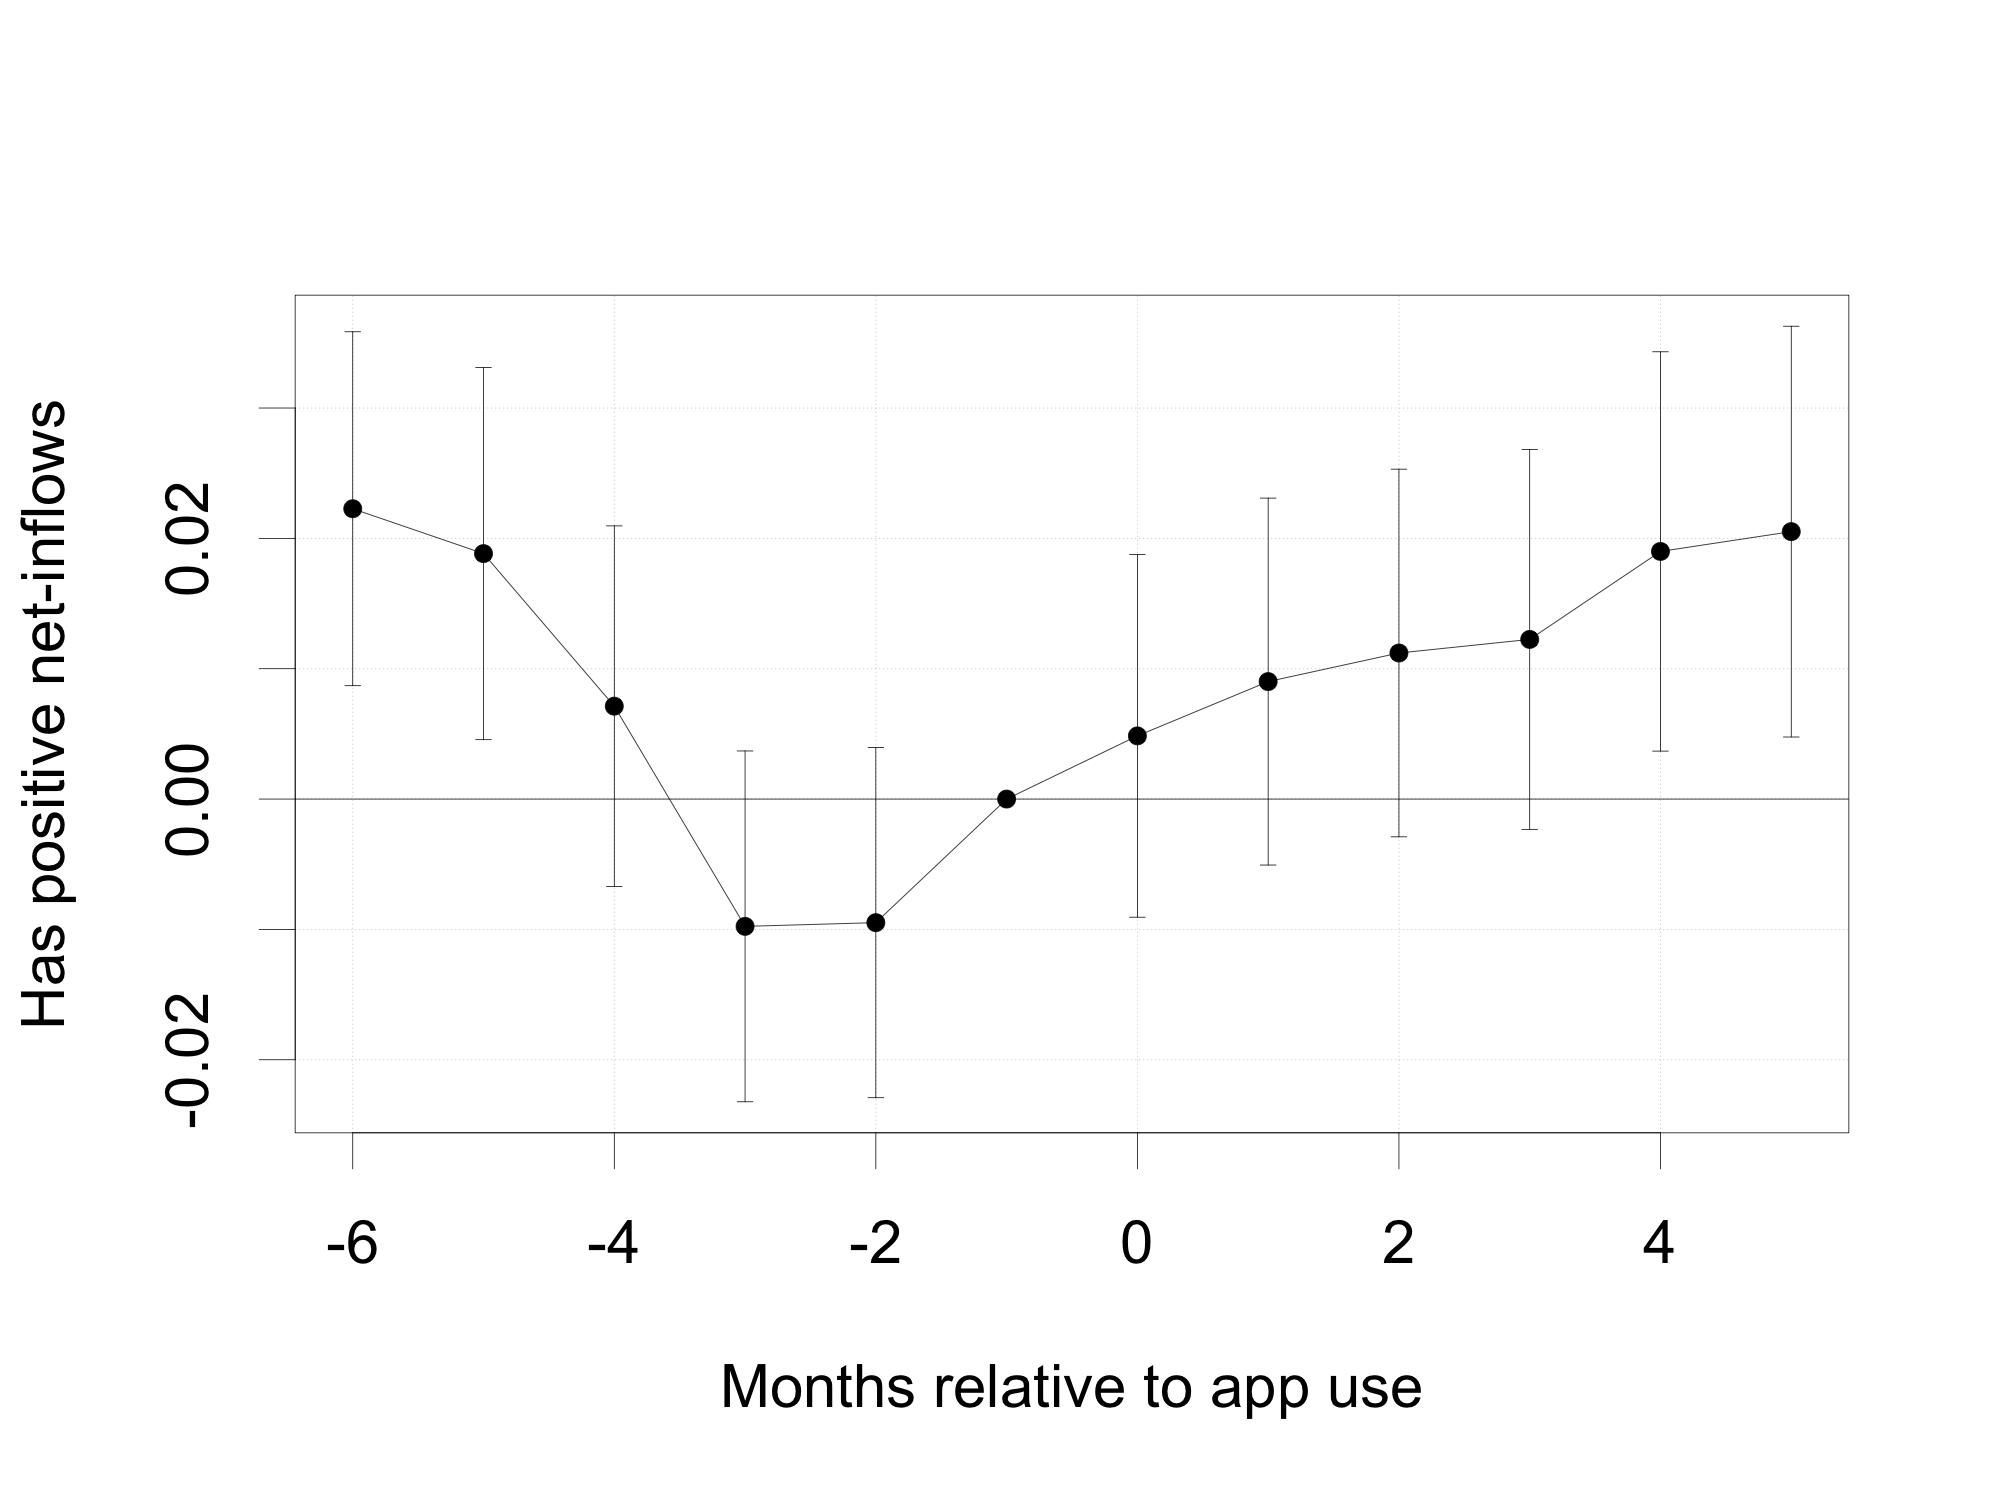
\includegraphics[width=.49\textwidth]{\figdir/has_pos_netflows.png}
    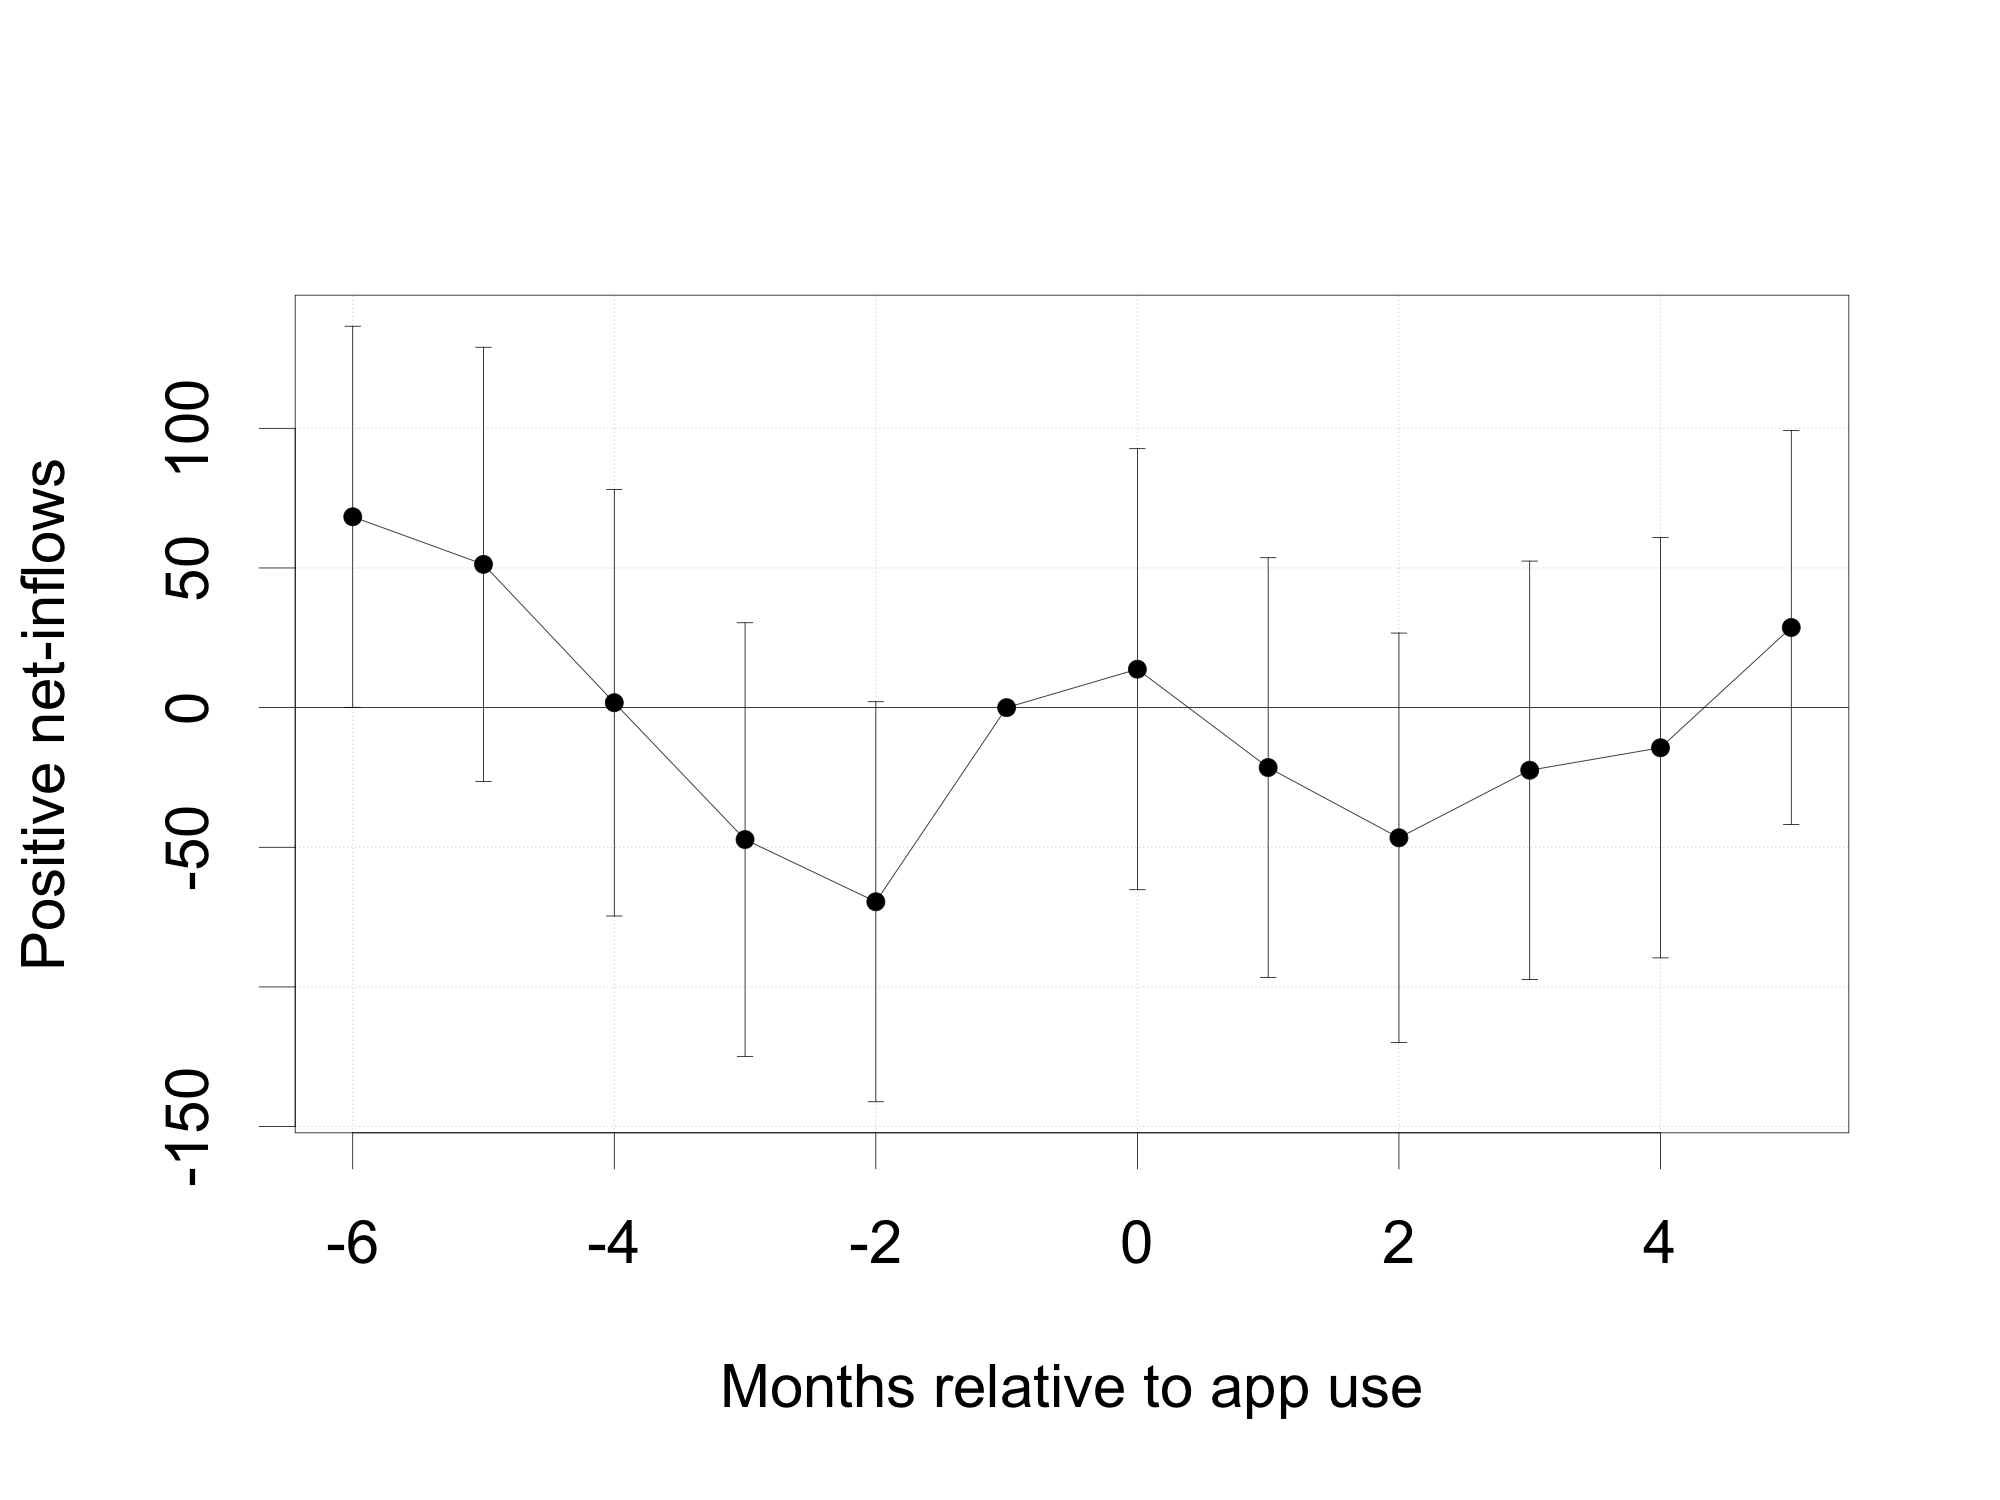
\includegraphics[width=.49\textwidth]{\figdir/pos_netflows.png}
    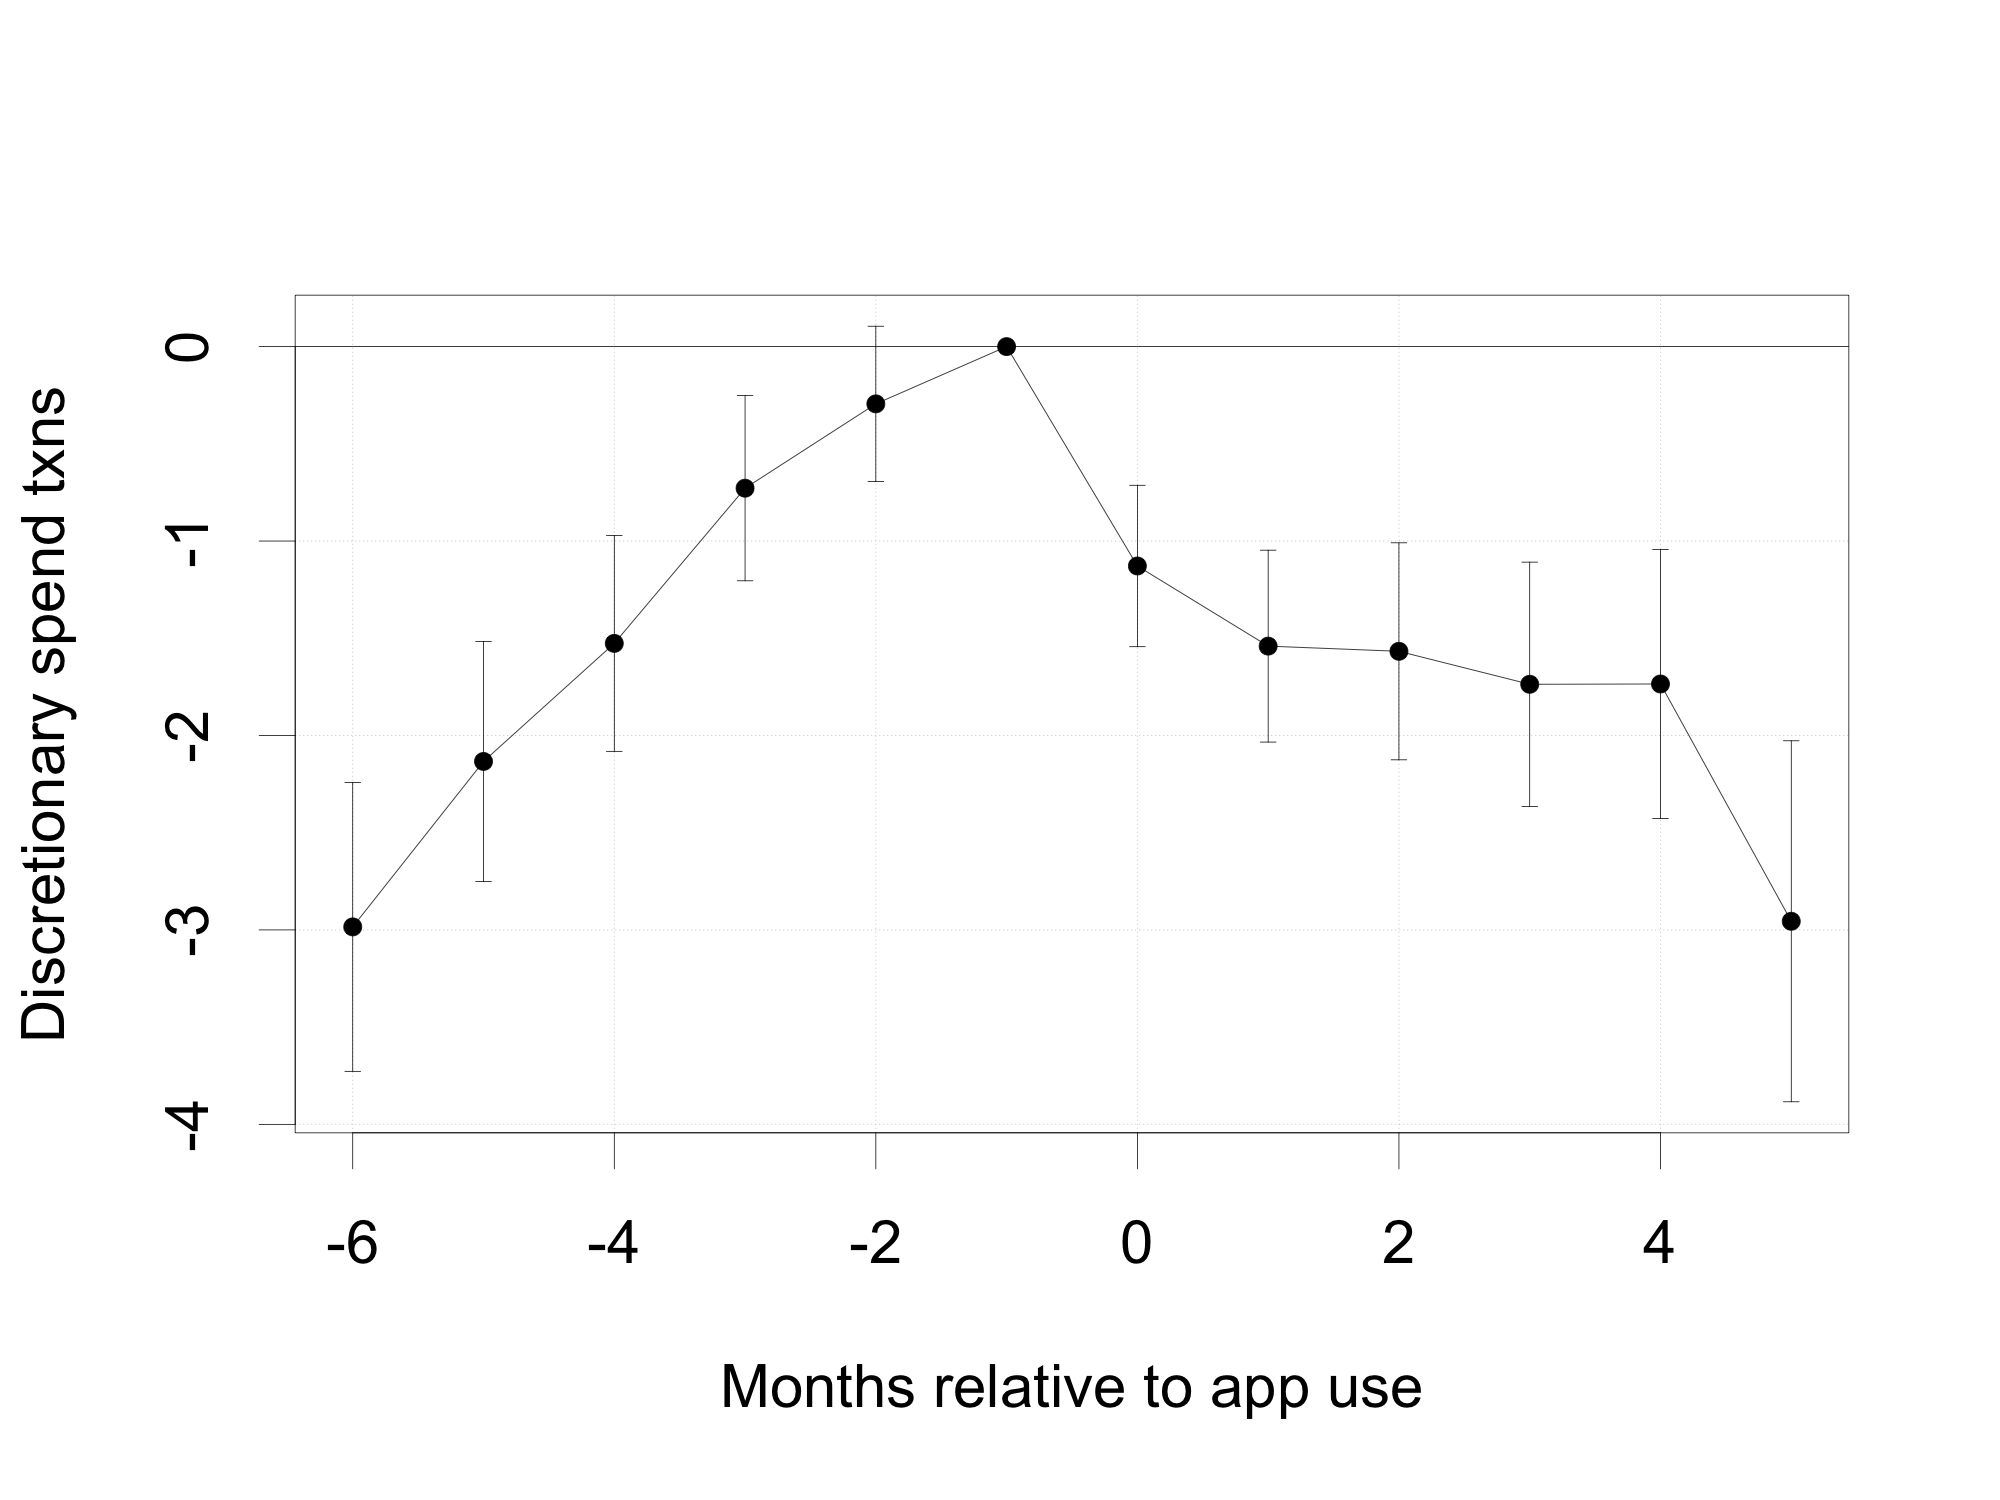
\includegraphics[width=.49\textwidth]{\figdir/dspend_count.png}
    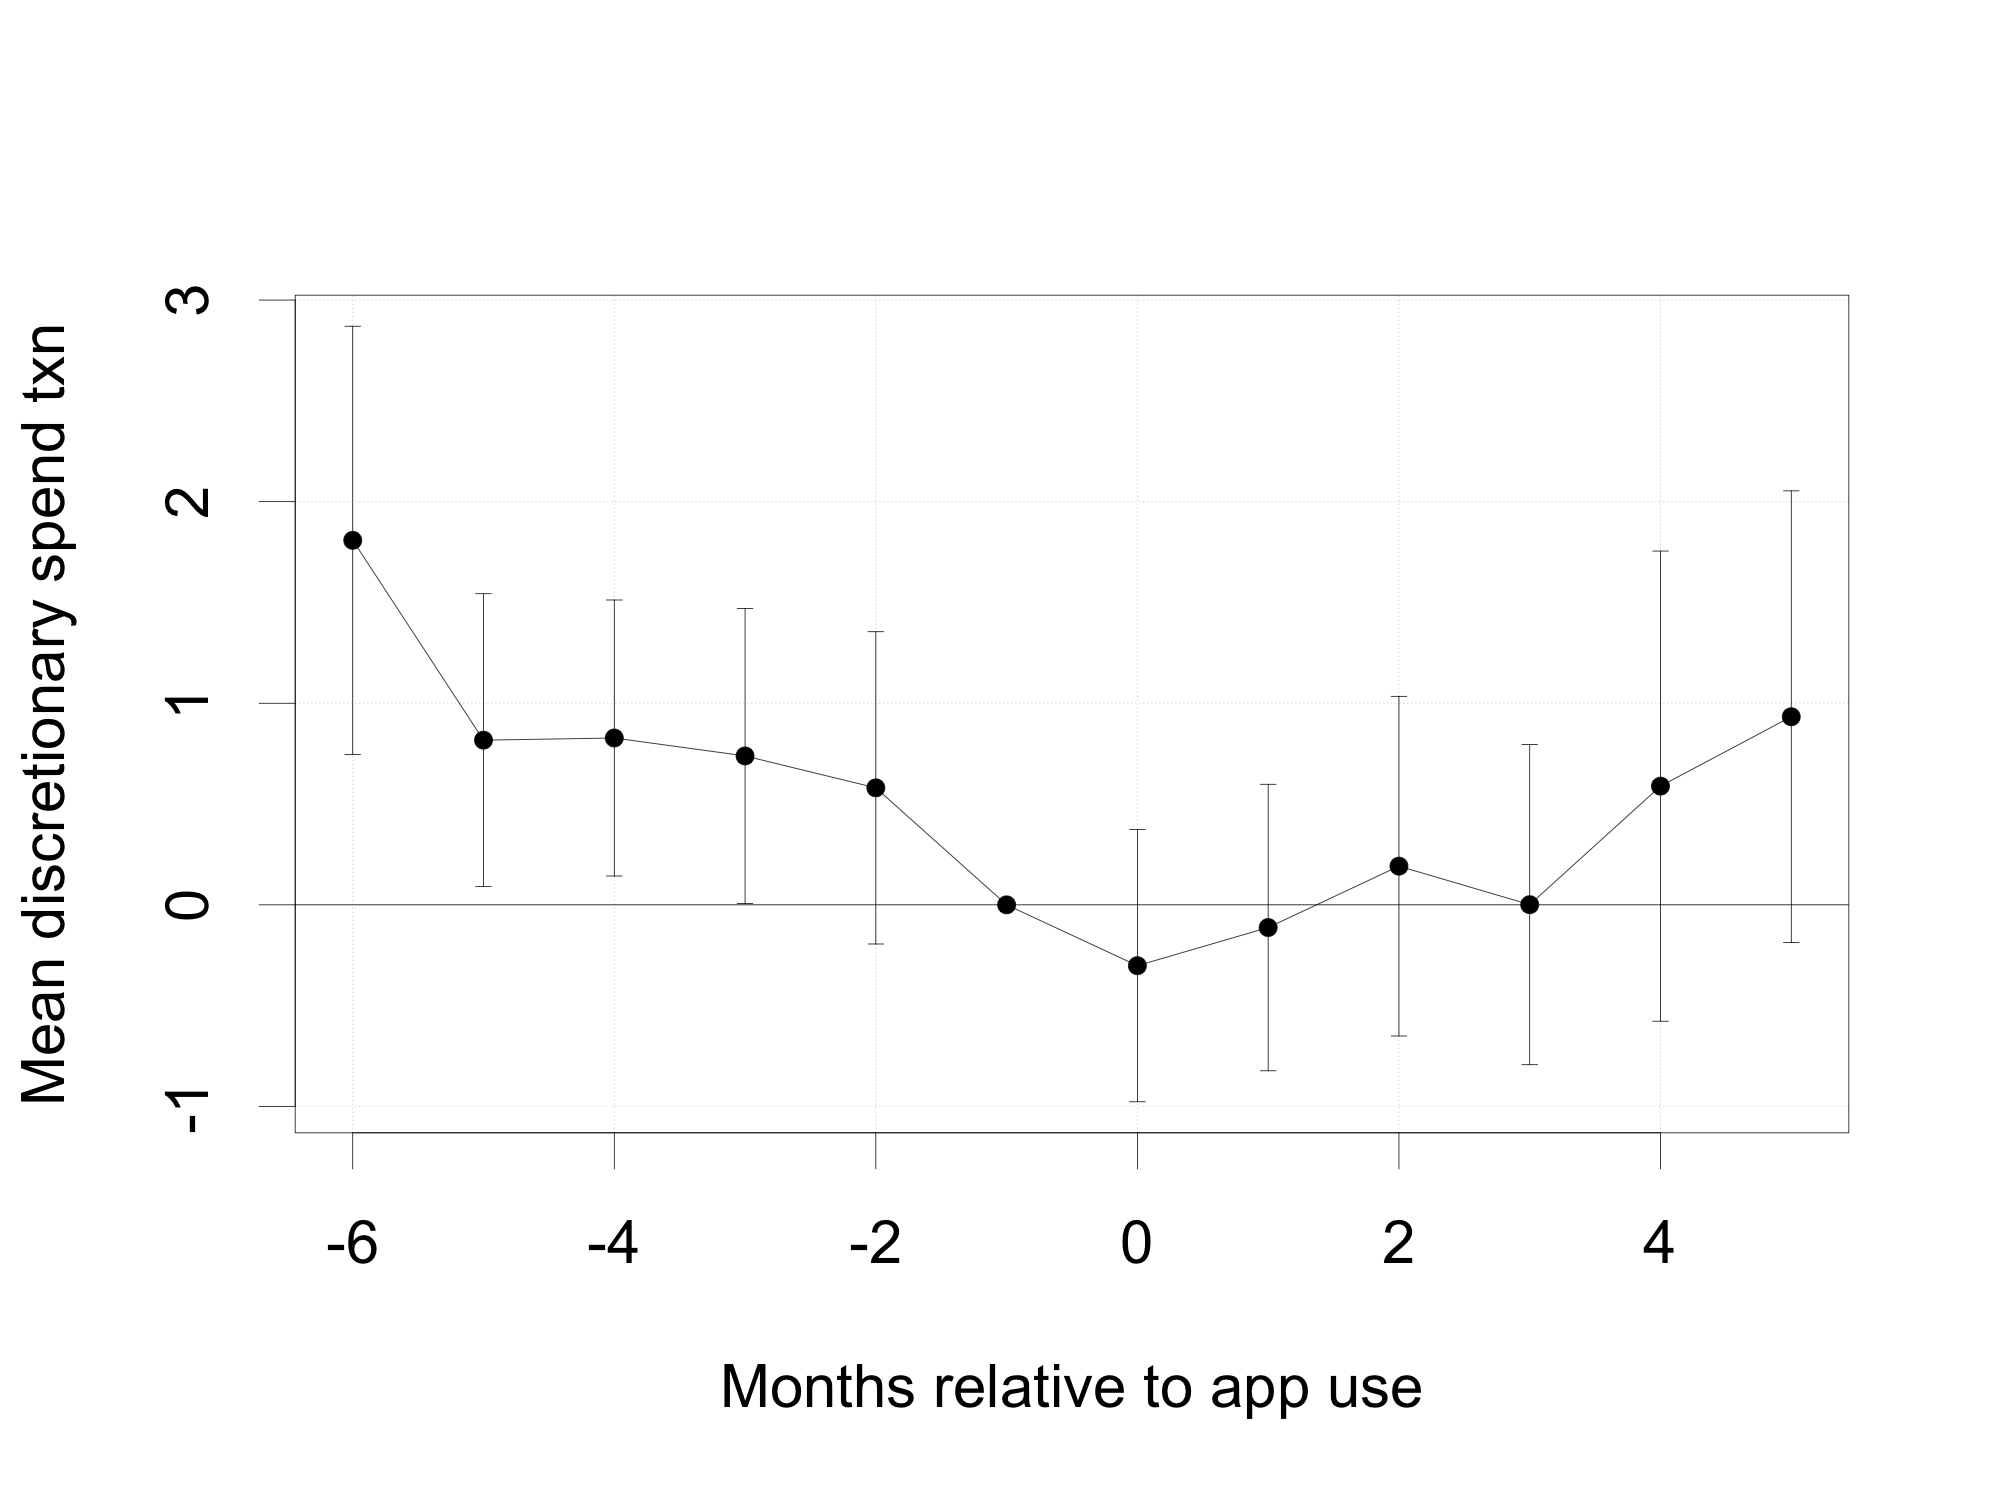
\includegraphics[width=.49\textwidth]{\figdir/dspend_mean.png}
    \fignote{\textwidth}{...}
\end{figure}


% 
\begin{table}[htbp]
   \centering
   \tiny
   \begin{threeparttable}[b]
      \caption{\label{tab:intext} Intensive and extensive margins}
      \begin{tabular}{lcccc}
         \tabularnewline \midrule \midrule
         Dependent Variables:              & Has positive net-inflows & Positive net-inflows & Discretionary spend txns & Mean discretionary spend txn\\  
         Model:                            & (1)                      & (2)                  & (3)                      & (4)\\  
         \midrule
         \emph{Variables}\\
         Months relative to app use $=$ -6 & 0.02$^{***}$             & 68.33$^{**}$         & -2.98$^{***}$            & 1.81$^{***}$\\   
                                           & [0.01; 0.04]             & [0.10; 136.56]       & [-3.73; -2.24]           & [0.75; 2.87]\\   
         Months relative to app use $=$ -5 & 0.02$^{***}$             & 51.29                & -2.13$^{***}$            & 0.82$^{**}$\\   
                                           & [0.00; 0.03]             & [-26.47; 129.04]     & [-2.75; -1.52]           & [0.09; 1.54]\\   
         Months relative to app use $=$ -4 & 0.01                     & 1.77                 & -1.53$^{***}$            & 0.83$^{**}$\\   
                                           & [-0.01; 0.02]            & [-74.62; 78.15]      & [-2.08; -0.97]           & [0.14; 1.51]\\   
         Months relative to app use $=$ -3 & -0.01                    & -47.23               & -0.73$^{***}$            & 0.74$^{**}$\\   
                                           & [-0.02; 0.00]            & [-124.87; 30.40]     & [-1.20; -0.25]           & [0.01; 1.47]\\   
         Months relative to app use $=$ -2 & -0.01                    & -69.51$^{*}$         & -0.29                    & 0.58\\   
                                           & [-0.02; 0.00]            & [-141.13; 2.11]      & [-0.69; 0.10]            & [-0.19; 1.35]\\   
         Months relative to app use $=$ 0  & 0.00                     & 13.75                & -1.13$^{***}$            & -0.30\\   
                                           & [-0.01; 0.02]            & [-65.21; 92.72]      & [-1.54; -0.71]           & [-0.98; 0.37]\\   
         Months relative to app use $=$ 1  & 0.01                     & -21.45               & -1.54$^{***}$            & -0.11\\   
                                           & [-0.01; 0.02]            & [-96.59; 53.68]      & [-2.03; -1.05]           & [-0.82; 0.60]\\   
         Months relative to app use $=$ 2  & 0.01                     & -46.60               & -1.57$^{***}$            & 0.19\\   
                                           & [-0.00; 0.03]            & [-119.91; 26.70]     & [-2.13; -1.01]           & [-0.65; 1.03]\\   
         Months relative to app use $=$ 3  & 0.01$^{*}$               & -22.42               & -1.74$^{***}$            & 0.00\\   
                                           & [-0.00; 0.03]            & [-97.31; 52.48]      & [-2.37; -1.11]           & [-0.79; 0.79]\\   
         Months relative to app use $=$ 4  & 0.02$^{**}$              & -14.37               & -1.74$^{***}$            & 0.59\\   
                                           & [0.00; 0.03]             & [-89.61; 60.87]      & [-2.43; -1.04]           & [-0.58; 1.76]\\   
         Months relative to app use $=$ 5  & 0.02$^{**}$              & 28.69                & -2.96$^{***}$            & 0.93\\   
                                           & [0.00; 0.04]             & [-41.84; 99.21]      & [-3.88; -2.03]           & [-0.19; 2.05]\\   
         Month income                      & 0.00$^{***}$             & 0.06$^{***}$         & 0.00$^{***}$             & -0.00$^{***}$\\   
                                           & [0.00; 0.00]             & [0.04; 0.08]         & [0.00; 0.00]             & [-0.00; -0.00]\\   
         Month spend                       & -0.00$^{***}$            & 0.02$^{***}$         & 0.00$^{***}$             & 0.00$^{***}$\\   
                                           & [-0.00; -0.00]           & [0.01; 0.03]         & [0.00; 0.00]             & [0.00; 0.00]\\   
         Active accounts                   & 0.09$^{***}$             & 184.51$^{***}$       & 3.41$^{***}$             & -0.87$^{***}$\\   
                                           & [0.09; 0.10]             & [170.36; 198.66]     & [3.21; 3.62]             & [-1.21; -0.53]\\   
         \midrule
         \emph{Fixed-effects}\\
         User ID                           & Yes                      & Yes                  & Yes                      & Yes\\  
         Year-month                        & Yes                      & Yes                  & Yes                      & Yes\\  
         \midrule
         \emph{Fit statistics}\\
         Observations                      & 188,324                  & 188,324              & 188,324                  & 187,306\\  
         R$^2$                             & 0.28475                  & 0.11551              & 0.68049                  & 0.26390\\  
         Within R$^2$                      & 0.06323                  & 0.01277              & 0.17182                  & 0.01562\\  
         \midrule \midrule
         \multicolumn{5}{l}{\emph{Clustered (User ID) co-variance matrix, 95\% confidence intervals in brackets}}\\
         \multicolumn{5}{l}{\emph{Signif. Codes: ***: 0.01, **: 0.05, *: 0.1}}\\
      \end{tabular}
   \end{threeparttable}
\end{table}





\subsection{Decomposing inflows and outflows}%
\label{sub:decomposing_inflows_and_outflows}

\begin{figure}[H]
    \centering
    \caption{Decomposing inflows and outflows}%
    \label{fig:inout}
    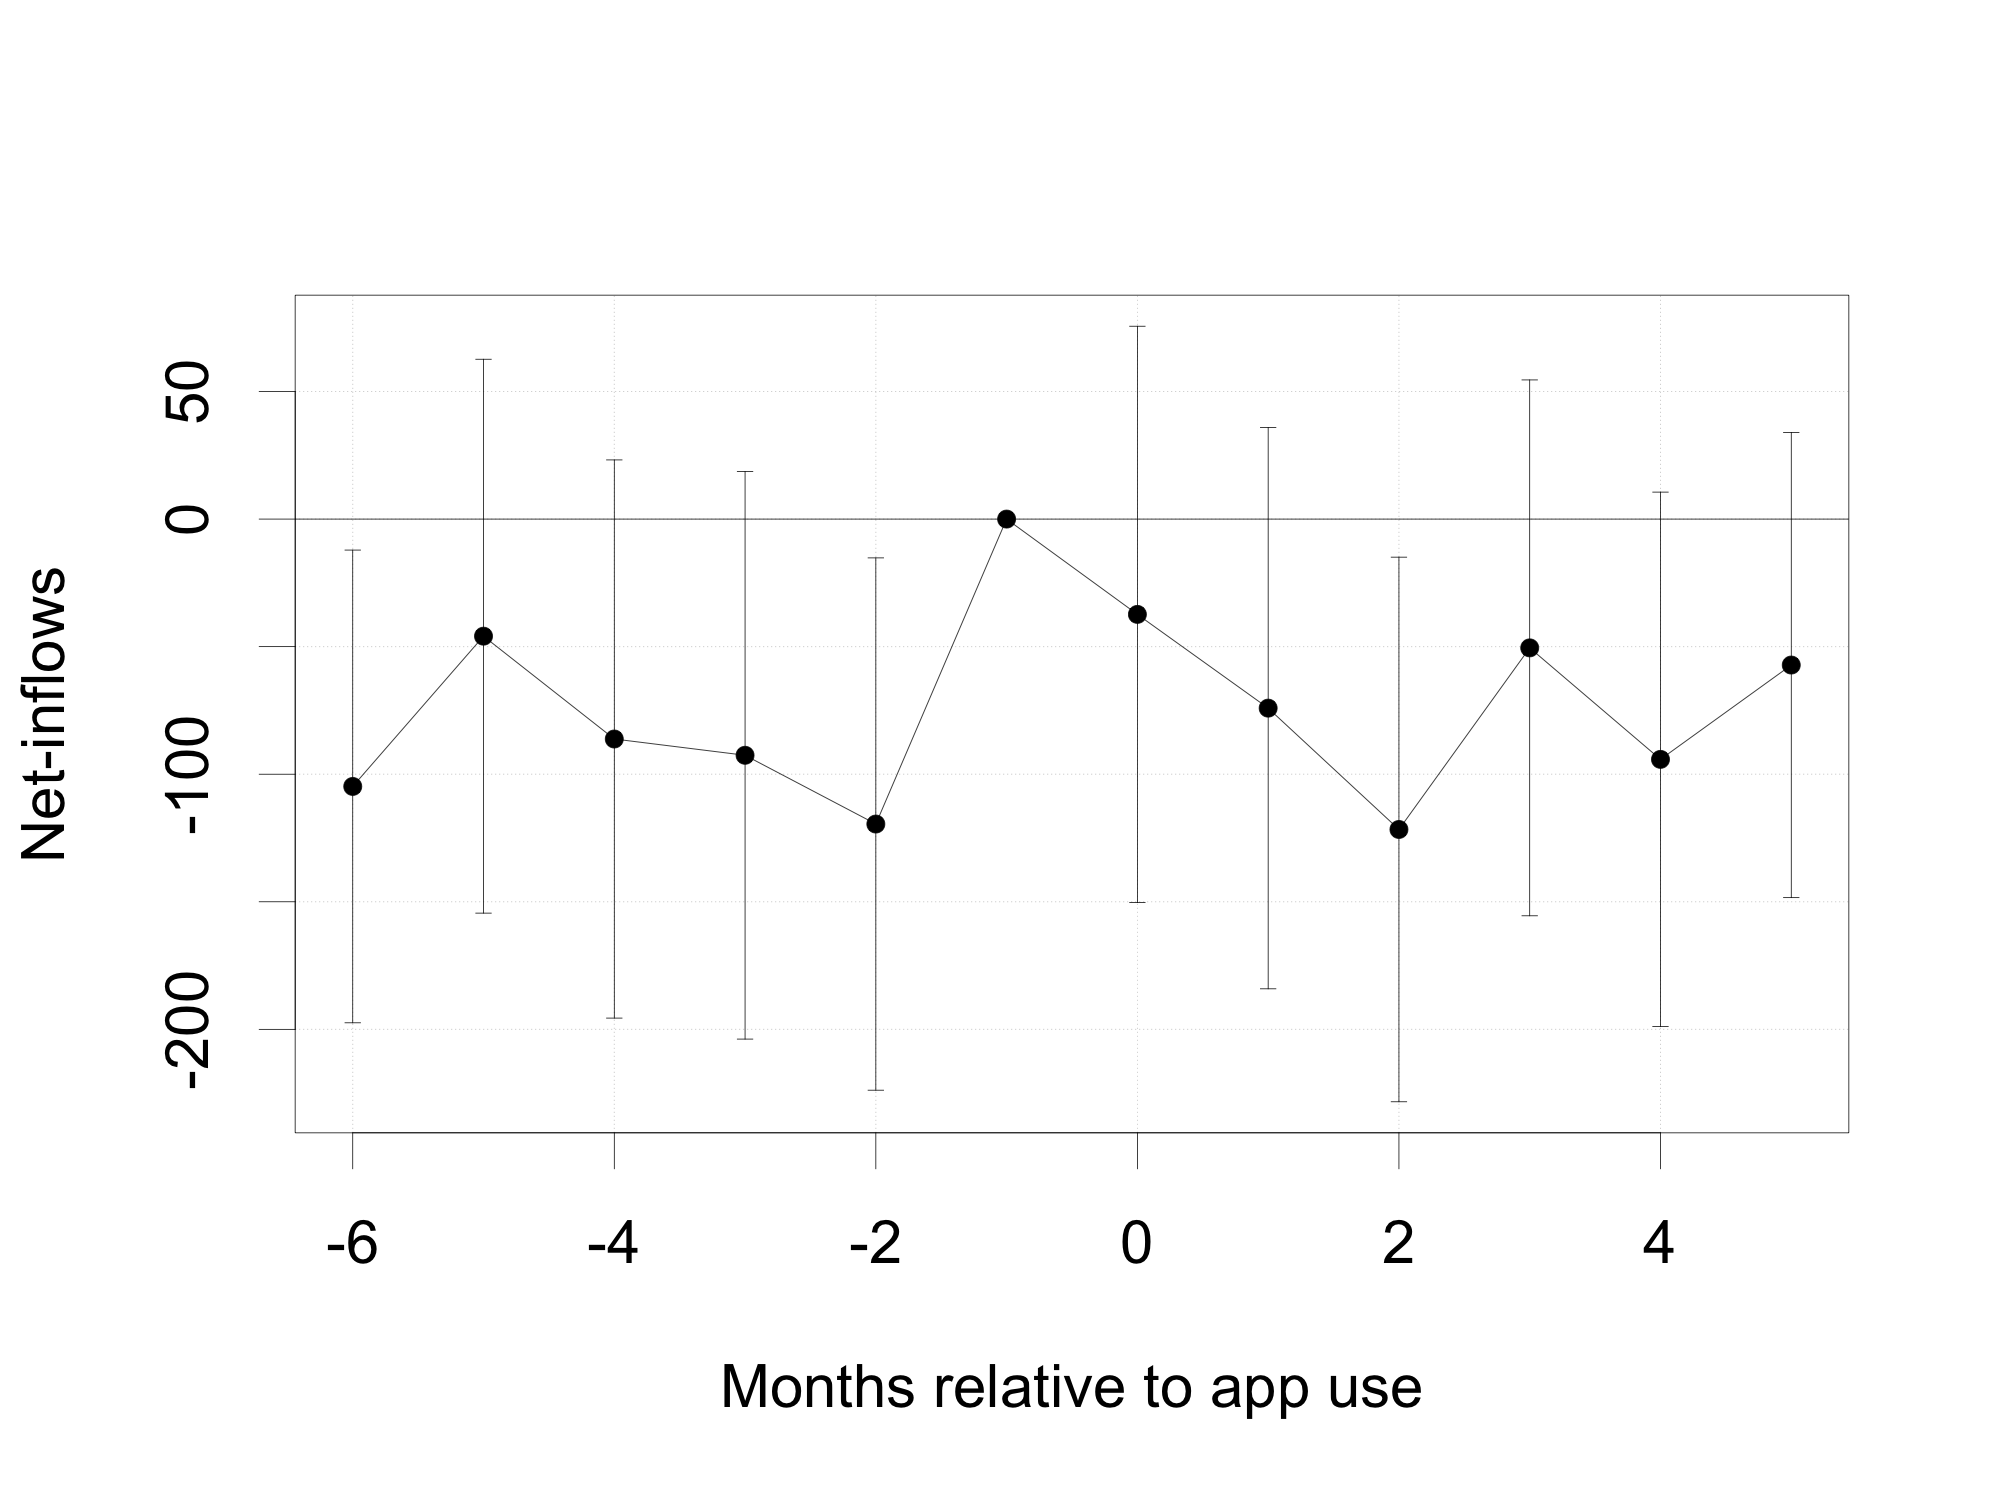
\includegraphics[width=.6\textwidth]{\figdir/netflows.png}
    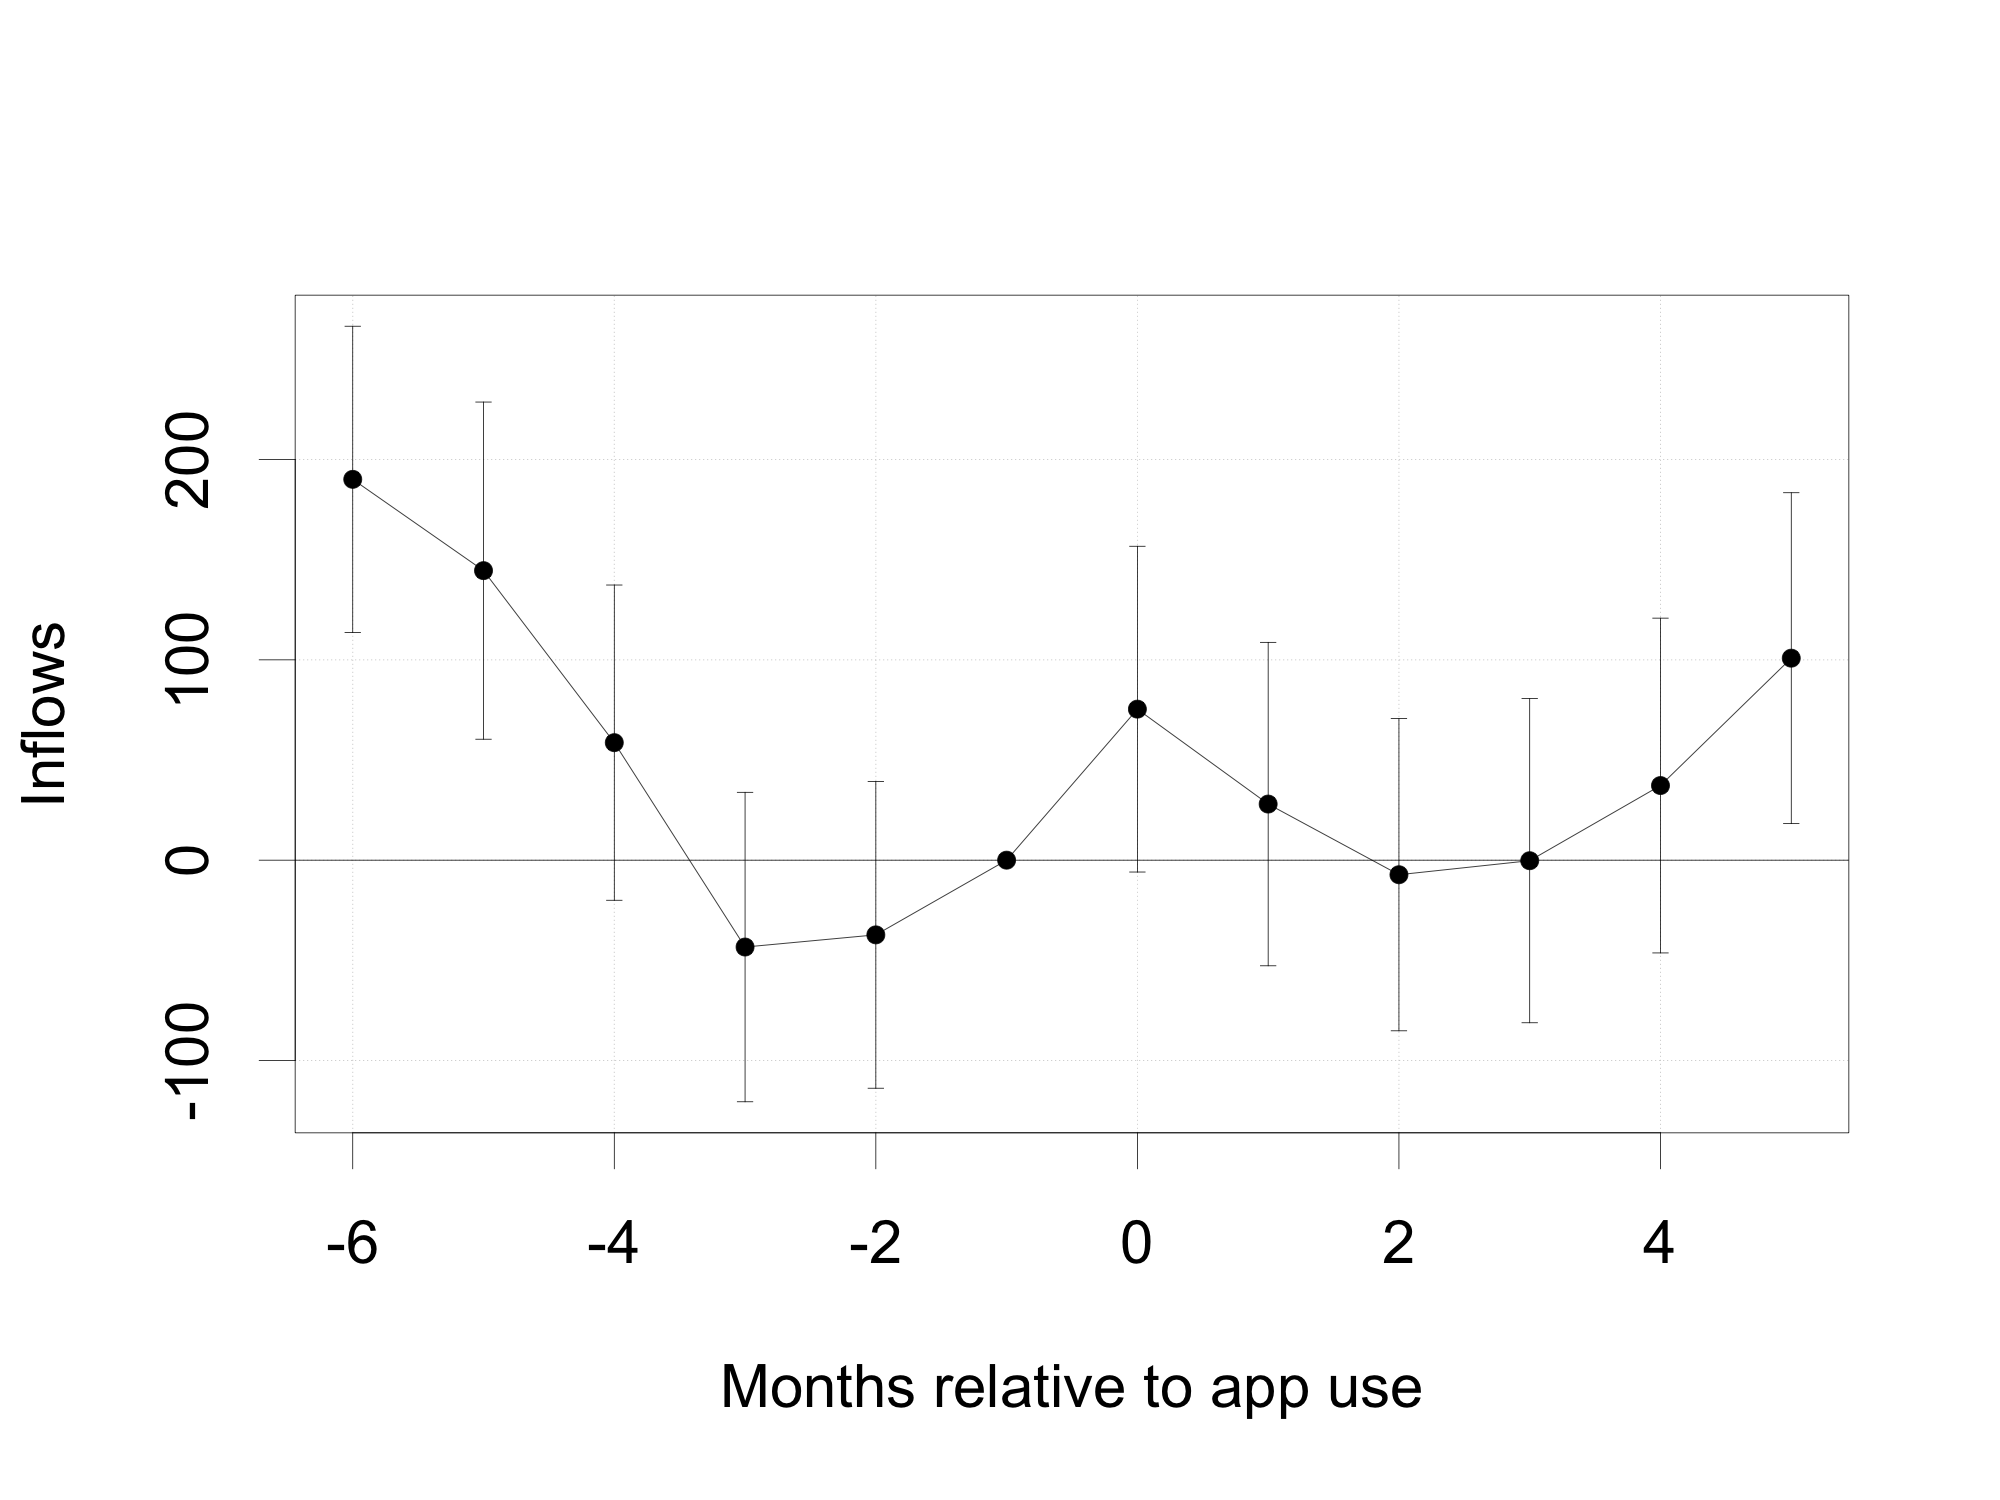
\includegraphics[width=.6\textwidth]{\figdir/inflows.png}
    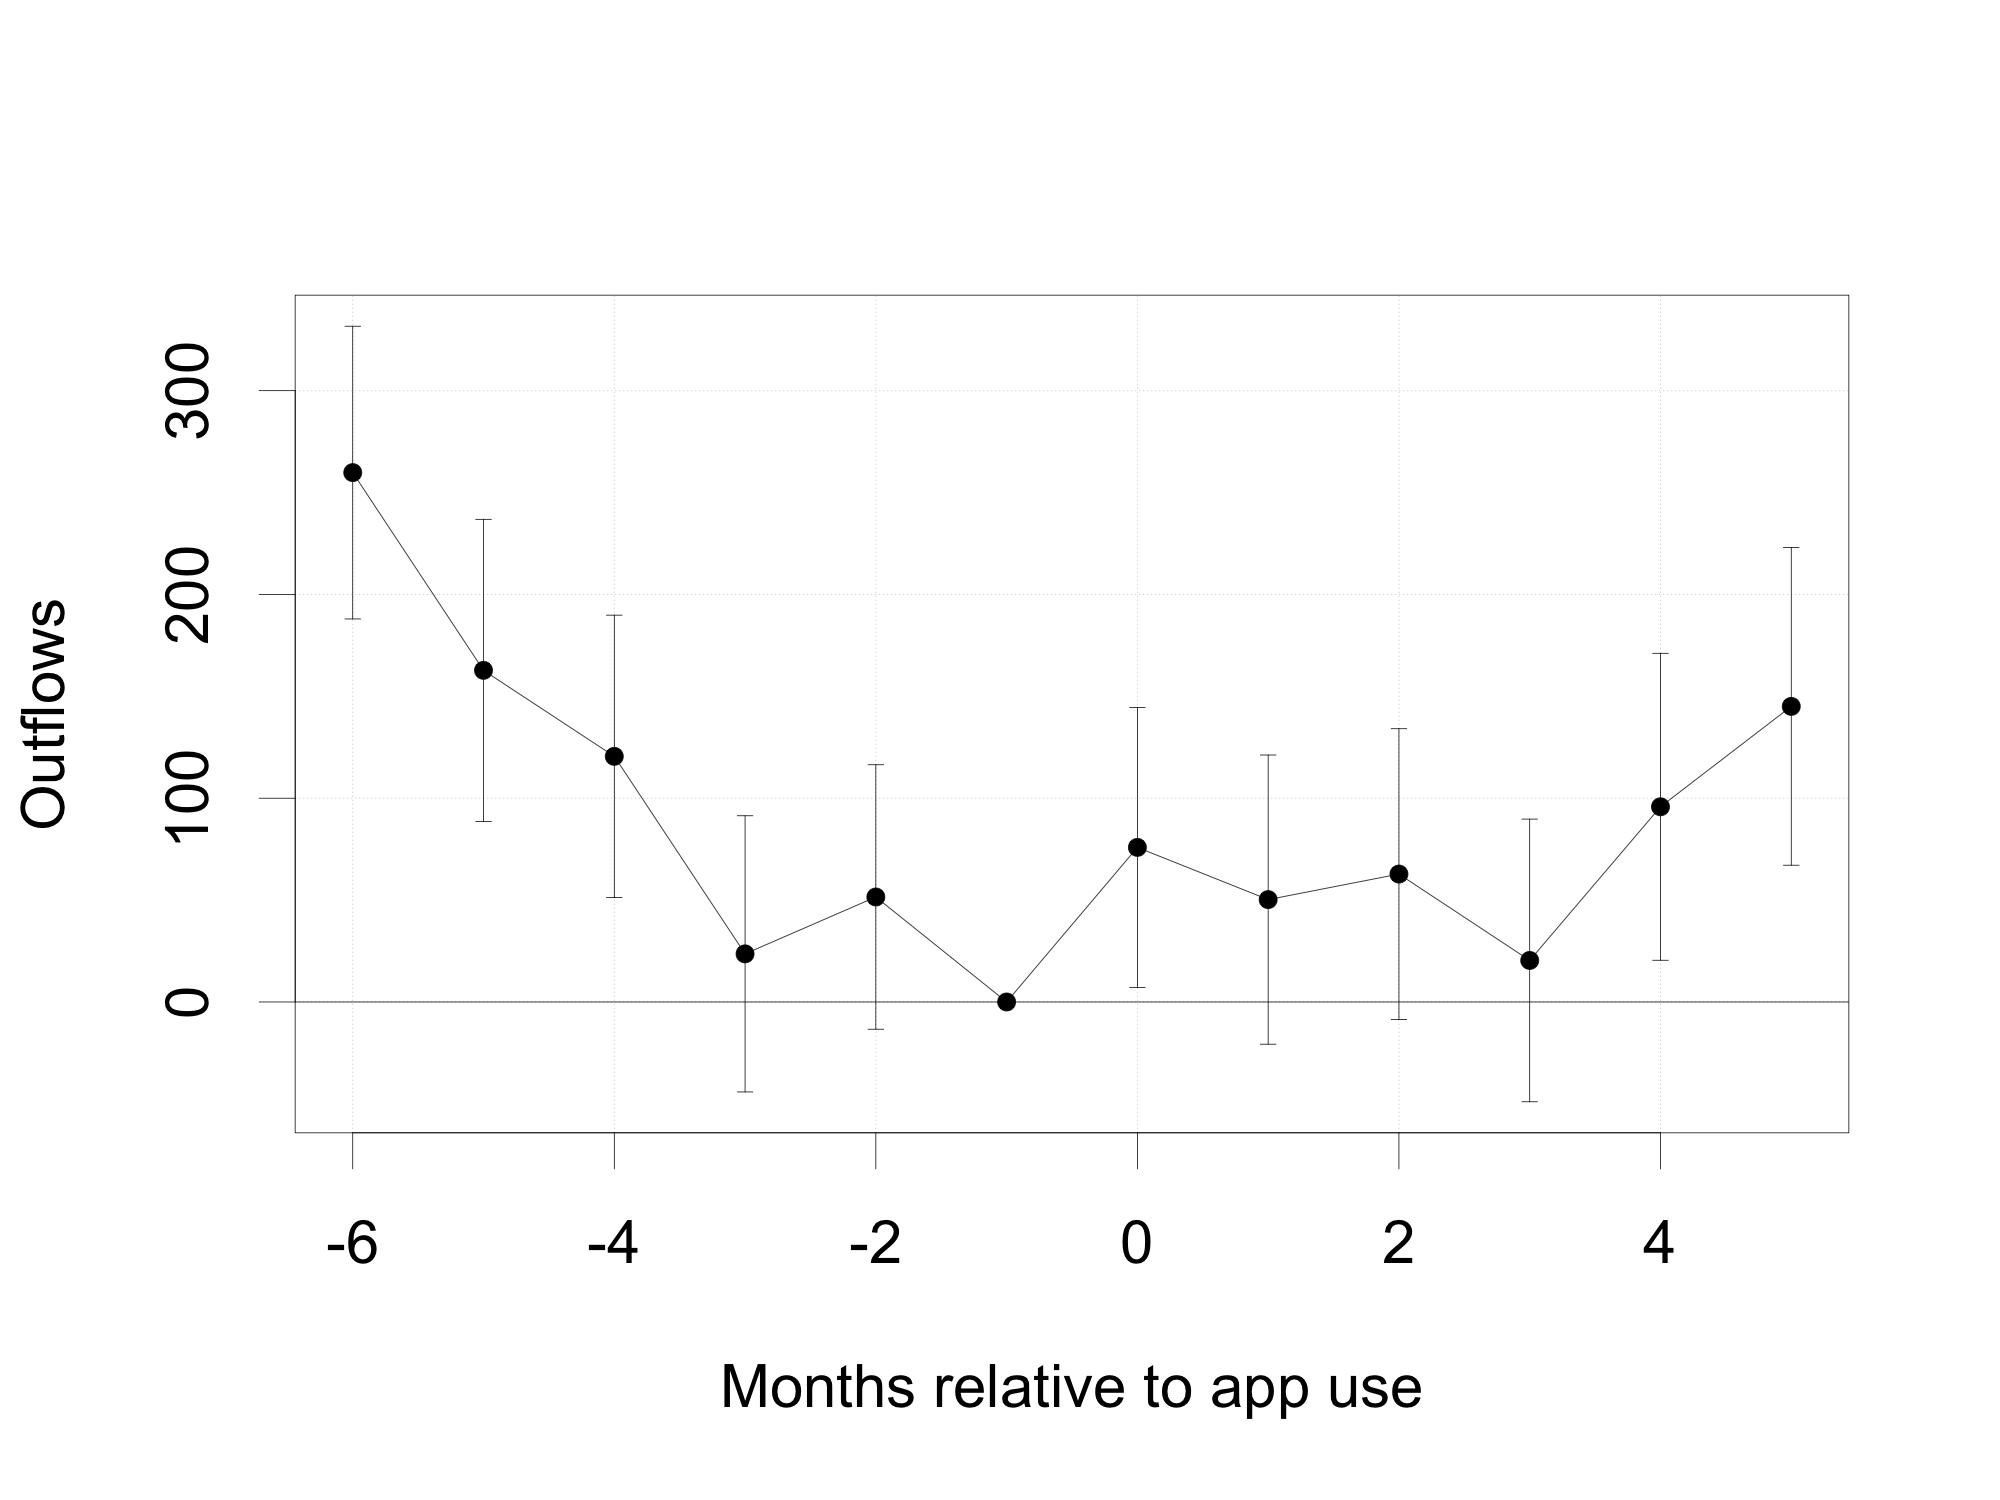
\includegraphics[width=.6\textwidth]{\figdir/outflows.png}
    \fignote{\textwidth}{...}
\end{figure}


\begin{table}[htbp]
   \centering
   \tiny
   \begin{threeparttable}[b]
      \caption{\label{tab:inout} Decomposing inflows and outflows}
      \begin{tabular}{lccc}
         \tabularnewline \midrule \midrule
         Dependent Variables:              & Net-inflows       & Inflows          & Outflows\\  
         Model:                            & (1)               & (2)              & (3)\\  
         \midrule
         \emph{Variables}\\
         Months relative to app use $=$ -6 & -104.79$^{**}$    & 190.11$^{***}$   & 259.80$^{***}$\\   
                                           & [-197.45; -12.13] & [113.66; 266.56] & [187.96; 331.64]\\   
         Months relative to app use $=$ -5 & -45.90            & 144.54$^{***}$   & 162.75$^{***}$\\   
                                           & [-154.47; 62.67]  & [60.37; 228.70]  & [88.62; 236.88]\\   
         Months relative to app use $=$ -4 & -86.20            & 58.67            & 120.54$^{***}$\\   
                                           & [-195.61; 23.21]  & [-20.02; 137.37] & [51.23; 189.85]\\   
         Months relative to app use $=$ -3 & -92.58            & -43.36           & 23.62\\   
                                           & [-203.84; 18.67]  & [-120.62; 33.89] & [-44.16; 91.39]\\   
         Months relative to app use $=$ -2 & -119.53$^{**}$    & -37.28           & 51.52\\   
                                           & [-223.87; -15.19] & [-113.85; 39.30] & [-13.38; 116.42]\\   
         Months relative to app use $=$ 0  & -37.36            & 75.39$^{*}$      & 75.86$^{**}$\\   
                                           & [-150.33; 75.61]  & [-5.93; 156.72]  & [7.16; 144.56]\\   
         Months relative to app use $=$ 1  & -74.11            & 28.01            & 50.24\\   
                                           & [-184.14; 35.92]  & [-52.74; 108.76] & [-20.73; 121.21]\\   
         Months relative to app use $=$ 2  & -121.66$^{**}$    & -7.26            & 62.77$^{*}$\\   
                                           & [-228.41; -14.90] & [-85.19; 70.68]  & [-8.57; 134.11]\\   
         Months relative to app use $=$ 3  & -50.48            & -0.26            & 20.39\\   
                                           & [-155.51; 54.56]  & [-81.18; 80.66]  & [-48.99; 89.77]\\   
         Months relative to app use $=$ 4  & -94.18$^{*}$      & 37.26            & 95.80$^{**}$\\   
                                           & [-198.96; 10.59]  & [-46.32; 120.84] & [20.47; 171.13]\\   
         Months relative to app use $=$ 5  & -57.21            & 100.83$^{**}$    & 145.05$^{***}$\\   
                                           & [-148.40; 33.97]  & [18.23; 183.44]  & [67.11; 223.00]\\   
         Month income                      & 0.08$^{***}$      & 0.06$^{***}$     & -0.01\\   
                                           & [0.05; 0.10]      & [0.04; 0.09]     & [-0.03; 0.02]\\   
         Month spend                       & -0.16$^{***}$     & 0.10$^{***}$     & 0.25$^{***}$\\   
                                           & [-0.19; -0.14]    & [0.08; 0.12]     & [0.23; 0.26]\\   
         Active accounts                   & 72.05$^{***}$     & 306.25$^{***}$   & 243.69$^{***}$\\   
                                           & [56.26; 87.84]    & [286.09; 326.40] & [224.27; 263.11]\\   
         \midrule
         \emph{Fixed-effects}\\
         User ID                           & Yes               & Yes              & Yes\\  
         Year-month                        & Yes               & Yes              & Yes\\  
         \midrule
         \emph{Fit statistics}\\
         Observations                      & 188,324           & 188,324          & 188,324\\  
         R$^2$                             & 0.04170           & 0.24635          & 0.31097\\  
         Within R$^2$                      & 0.01007           & 0.03612          & 0.07191\\  
         \midrule \midrule
         \multicolumn{4}{l}{\emph{Clustered (User ID) co-variance matrix, 95\% confidence intervals in brackets}}\\
         \multicolumn{4}{l}{\emph{Signif. Codes: ***: 0.01, **: 0.05, *: 0.1}}\\
      \end{tabular}
   \end{threeparttable}
\end{table}






\subsection{Static results}%
\label{sub:static_results}


\begin{table}[htbp]
   \centering
   \tiny
   \begin{threeparttable}[b]
      \caption{\label{tab:static} Static results}
      \begin{tabular}{lcccccccc}
         \tabularnewline \midrule \midrule
         Dependent Variables: & \multicolumn{4}{c}{Net-inflows} & \multicolumn{4}{c}{Discretionary spend}\\
         Model:          & (1)             & (2)            & (3)             & (4)             & (5)              & (6)            & (7)             & (8)\\  
         \midrule
         \emph{Variables}\\
         App use         & 37.93$^{***}$   & 27.14$^{**}$   & 5.60            & -0.08           & 69.09$^{***}$    & 49.57$^{***}$  & 1.05            & -26.59$^{***}$\\   
                         & [11.16; 64.71]  & [0.73; 53.55]  & [-26.57; 37.78] & [-50.70; 50.55] & [63.78; 74.40]   & [41.46; 57.69] & [-12.92; 15.03] & [-38.73; -14.45]\\   
         Month income    & 0.07$^{***}$    & 0.07$^{***}$   & 0.07$^{***}$    & 0.08$^{***}$    & 0.02$^{***}$     & 0.01$^{***}$   & 0.02$^{***}$    & 0.01$^{***}$\\   
                         & [0.06; 0.08]    & [0.05; 0.10]   & [0.05; 0.09]    & [0.05; 0.10]    & [0.02; 0.02]     & [0.01; 0.02]   & [0.02; 0.03]    & [0.00; 0.02]\\   
         Month spend     & -0.12$^{***}$   & -0.16$^{***}$  & -0.12$^{***}$   & -0.16$^{***}$   & 0.16$^{***}$     & 0.12$^{***}$   & 0.16$^{***}$    & 0.12$^{***}$\\   
                         & [-0.13; -0.11]  & [-0.19; -0.14] & [-0.14; -0.10]  & [-0.19; -0.14]  & [0.16; 0.16]     & [0.11; 0.12]   & [0.15; 0.17]    & [0.11; 0.12]\\   
         Active accounts & 40.31$^{***}$   & 75.54$^{***}$  & 38.87$^{***}$   & 73.25$^{***}$   & 45.89$^{***}$    & 85.71$^{***}$  & 42.11$^{***}$   & 74.92$^{***}$\\   
                         & [32.66; 47.95]  & [60.63; 90.45] & [25.50; 52.23]  & [57.69; 88.81]  & [44.37; 47.40]   & [81.21; 90.20] & [39.61; 44.60]  & [70.47; 79.38]\\   
         Intercept       & -7.11           &                &                 &                 & 172.15$^{***}$   &                &                 &   \\   
                         & [-37.67; 23.45] &                &                 &                 & [166.09; 178.21] &                &                 &   \\   
         \midrule
         \emph{Fixed-effects}\\
         User ID         &                 & Yes            &                 & Yes             &                  & Yes            &                 & Yes\\  
         Year-month      &                 &                & Yes             & Yes             &                  &                & Yes             & Yes\\  
         \midrule
         \emph{Fit statistics}\\
         Observations    & 188,324         & 188,324        & 188,324         & 188,324         & 188,324          & 188,324        & 188,324         & 188,324\\  
         R$^2$           & 0.00888         & 0.04113        & 0.00940         & 0.04163         & 0.41618          & 0.66171        & 0.42425         & 0.67060\\  
         Within R$^2$    &                 & 0.01014        & 0.00877         & 0.01000         &                  & 0.28046        & 0.40985         & 0.23849\\  
         \midrule \midrule
         \multicolumn{9}{l}{\emph{Signif. Codes: ***: 0.01, **: 0.05, *: 0.1}}\\
      \end{tabular}
   \end{threeparttable}
\end{table}






\subsection{Additional TWFE specifications}%
\label{sub:additional_twfe_specifications}

\begin{figure}[H]
    \centering
    \caption{Alternative model specifications}%
    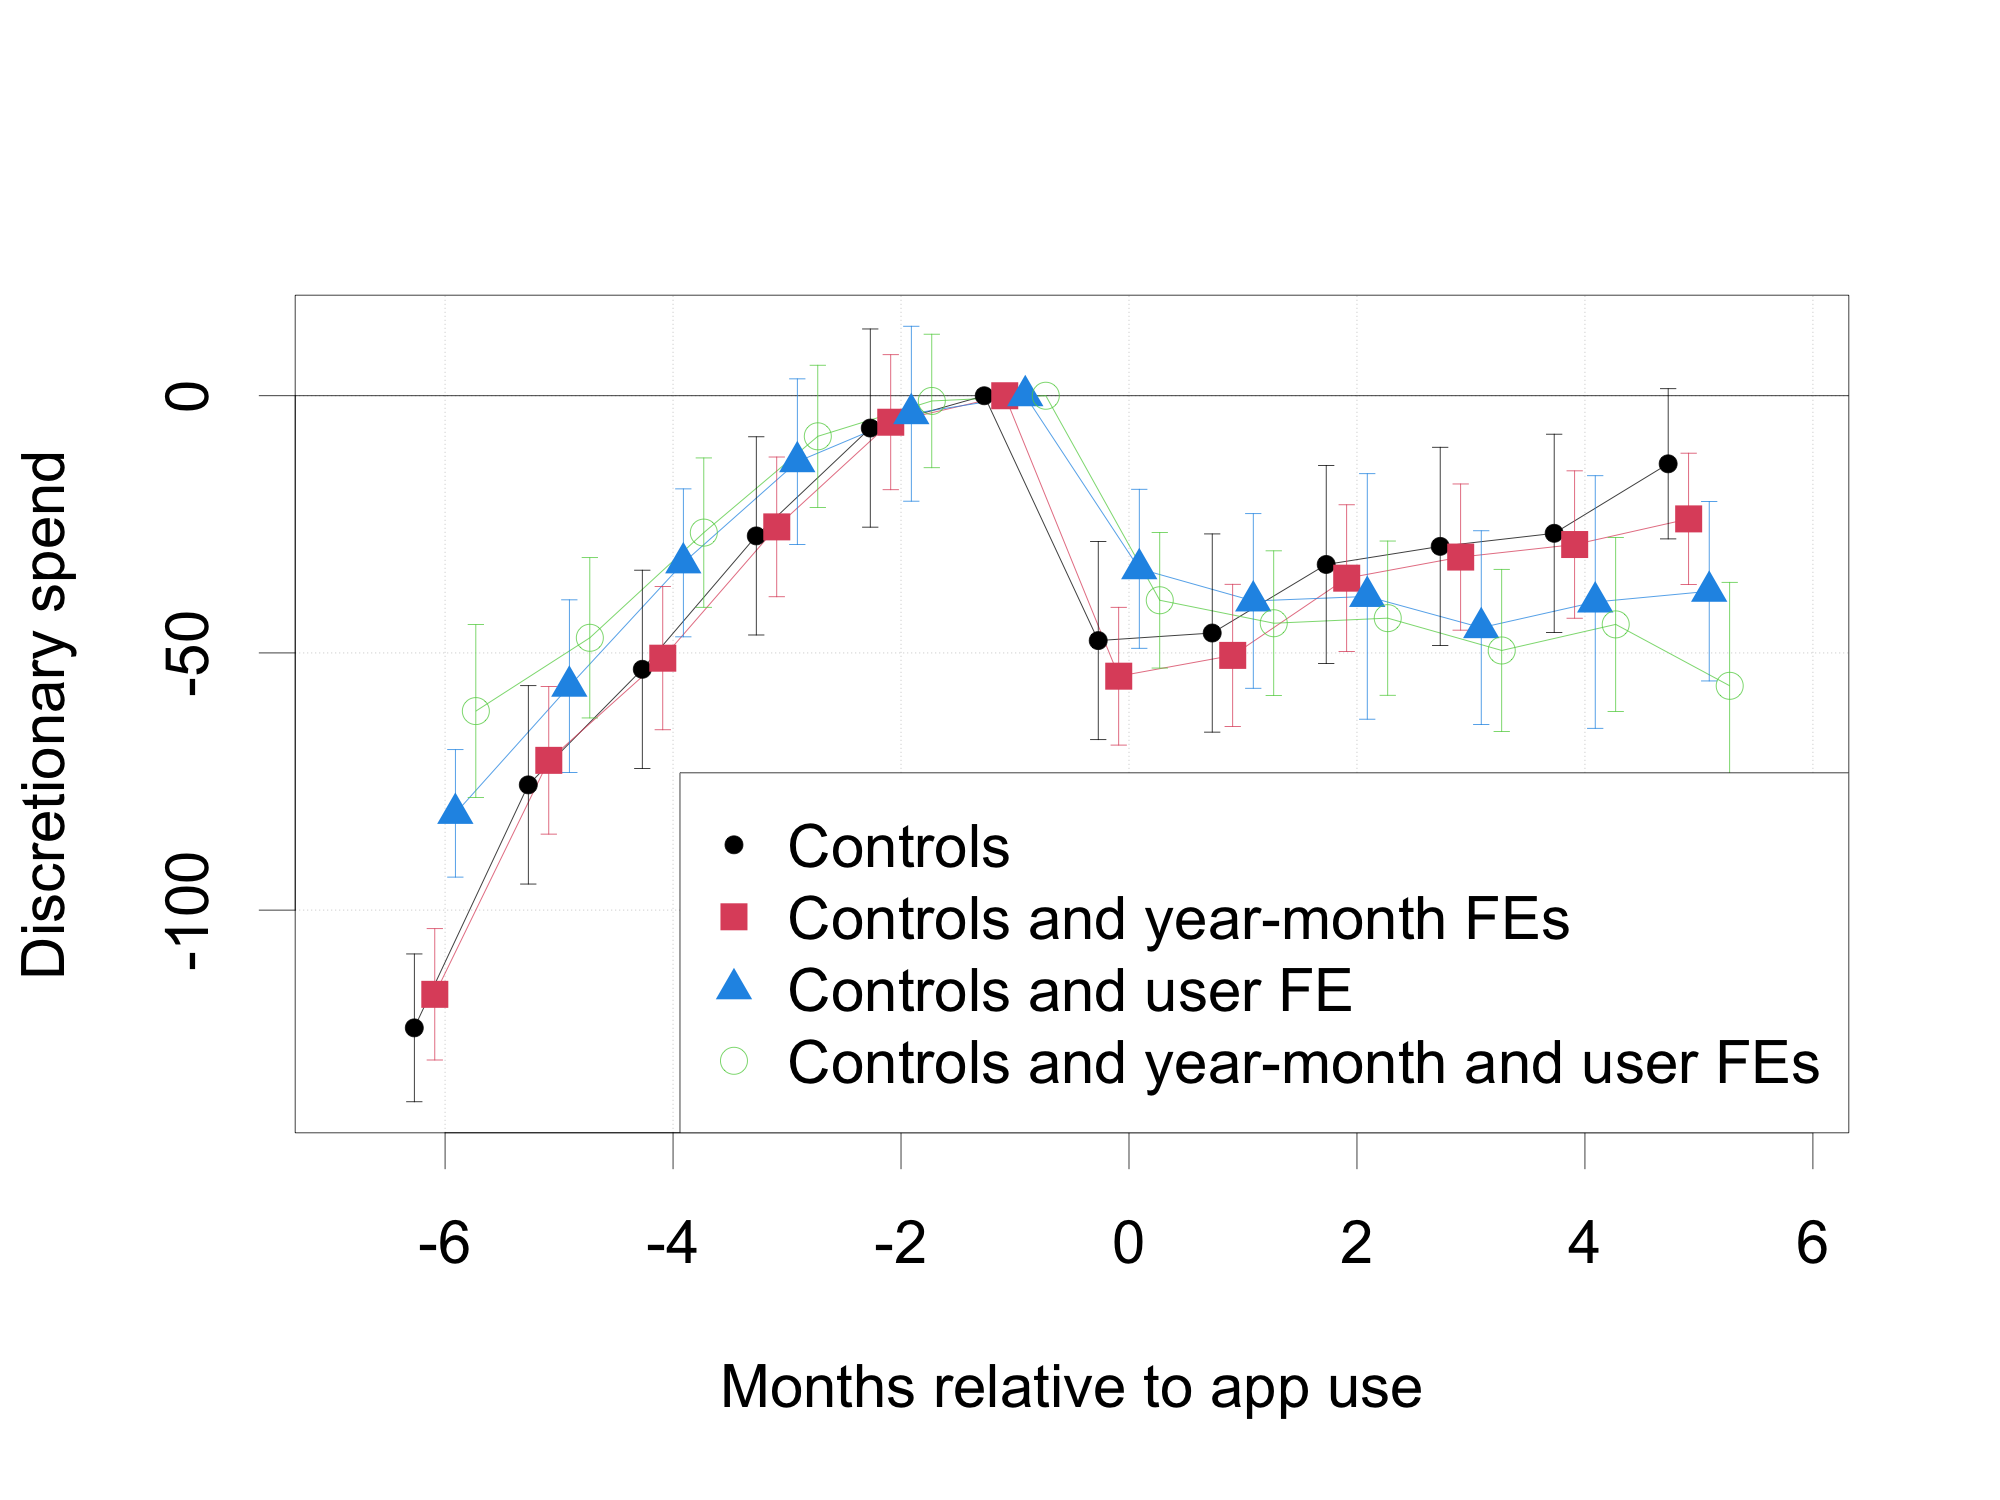
\includegraphics[width=.7\textwidth]{\figdir/dspend_alt.png}
\end{figure}


\begin{table}[htbp]
   \centering
   \tiny
   \begin{threeparttable}[b]
      \caption{\label{tab:dspend_alt} Alternative model specifications}
      \begin{tabular}{lcccc}
         \tabularnewline \midrule \midrule
         Dependent Variable: & \multicolumn{4}{c}{Discretionary spend}\\
         Model:                            & (1)                & (2)                & (3)              & (4)\\  
         \midrule
         \emph{Variables}\\
         Months relative to app use $=$ -6 & -122.89$^{***}$    & -116.38$^{***}$    & -81.19$^{***}$   & -61.31$^{***}$\\   
                                           & [-137.26; -108.52] & [-129.14; -103.61] & [-93.92; -68.47] & [-78.13; -44.48]\\   
         Months relative to app use $=$ -5 & -75.65$^{***}$     & -70.88$^{***}$     & -56.47$^{***}$   & -47.06$^{***}$\\   
                                           & [-94.93; -56.37]   & [-85.23; -56.54]   & [-73.72; -39.23] & [-62.64; -31.47]\\   
         Months relative to app use $=$ -4 & -53.18$^{***}$     & -51.02$^{***}$     & -32.49$^{***}$   & -26.61$^{***}$\\   
                                           & [-72.45; -33.91]   & [-64.94; -37.10]   & [-47.26; -17.72] & [-41.13; -12.09]\\   
         Months relative to app use $=$ -3 & -27.25$^{***}$     & -25.50$^{***}$     & -12.83           & -7.89\\   
                                           & [-46.51; -7.98]    & [-39.08; -11.91]   & [-29.37; 3.72]   & [-21.71; 5.94]\\   
         Months relative to app use $=$ -2 & -6.28              & -5.15              & -3.49            & -1.01\\   
                                           & [-25.55; 12.98]    & [-18.28; 7.98]     & [-20.95; 13.98]  & [-13.00; 11.97]\\   
         Months relative to app use $=$ 0  & -47.60$^{***}$     & -54.52$^{***}$     & -33.64$^{***}$   & -39.76$^{***}$\\   
                                           & [-66.86; -28.34]   & [-67.92; -41.12]   & [-49.51; -17.76] & [-52.94; -26.58]\\   
         Months relative to app use $=$ 1  & -46.13$^{***}$     & -50.48$^{***}$     & -39.90$^{***}$   & -44.23$^{***}$\\   
                                           & [-65.40; -26.86]   & [-64.31; -36.65]   & [-57.33; -22.47] & [-58.30; -30.15]\\   
         Months relative to app use $=$ 2  & -32.80$^{***}$     & -35.47$^{***}$     & -39.02$^{***}$   & -43.24$^{***}$\\   
                                           & [-52.07; -13.53]   & [-49.73; -21.20]   & [-63.52; -14.51] & [-58.23; -28.24]\\   
         Months relative to app use $=$ 3  & -29.28$^{***}$     & -31.36$^{***}$     & -45.09$^{***}$   & -49.52$^{***}$\\   
                                           & [-48.56; -10.01]   & [-45.57; -17.15]   & [-64.44; -25.75] & [-65.30; -33.74]\\   
         Months relative to app use $=$ 4  & -26.75$^{***}$     & -28.93$^{***}$     & -40.10$^{***}$   & -44.45$^{***}$\\   
                                           & [-46.02; -7.47]    & [-43.25; -14.60]   & [-65.31; -14.89] & [-61.37; -27.53]\\   
         Months relative to app use $=$ 5  & -13.23$^{*}$       & -23.94$^{***}$     & -38.01$^{***}$   & -56.39$^{***}$\\   
                                           & [-27.83; 1.37]     & [-36.72; -11.16]   & [-55.92; -20.11] & [-76.52; -36.27]\\   
         Month income                      & 0.02$^{***}$       & 0.01$^{***}$       & 0.02$^{***}$     & 0.01$^{***}$\\   
                                           & [0.02; 0.03]       & [0.01; 0.02]       & [0.02; 0.03]     & [0.00; 0.02]\\   
         Month spend                       & 0.16$^{***}$       & 0.12$^{***}$       & 0.16$^{***}$     & 0.12$^{***}$\\   
                                           & [0.16; 0.16]       & [0.11; 0.12]       & [0.15; 0.17]     & [0.11; 0.12]\\   
         Active accounts                   & 41.94$^{***}$      & 77.85$^{***}$      & 40.80$^{***}$    & 72.39$^{***}$\\   
                                           & [40.39; 43.49]     & [73.30; 82.41]     & [38.37; 43.22]   & [67.89; 76.88]\\   
         Intercept                         & 274.97$^{***}$     &                    &                  &   \\   
                                           & [260.03; 289.91]   &                    &                  &   \\   
         \midrule
         \emph{Fixed-effects}\\
         User ID                           &                    & Yes                &                  & Yes\\  
         Year-month                        &                    &                    & Yes              & Yes\\  
         \midrule
         \emph{Fit statistics}\\
         Observations                      & 188,324            & 188,324            & 188,324          & 188,324\\  
         R$^2$                             & 0.41828            & 0.66337            & 0.42491          & 0.67097\\  
         Within R$^2$                      &                    & 0.28398            & 0.41052          & 0.23935\\  
         \midrule \midrule
         \multicolumn{5}{l}{\emph{Signif. Codes: ***: 0.01, **: 0.05, *: 0.1}}\\
      \end{tabular}
   \end{threeparttable}
\end{table}





\begin{figure}[H]
    \centering
    \caption{Alternative model specifications}%
    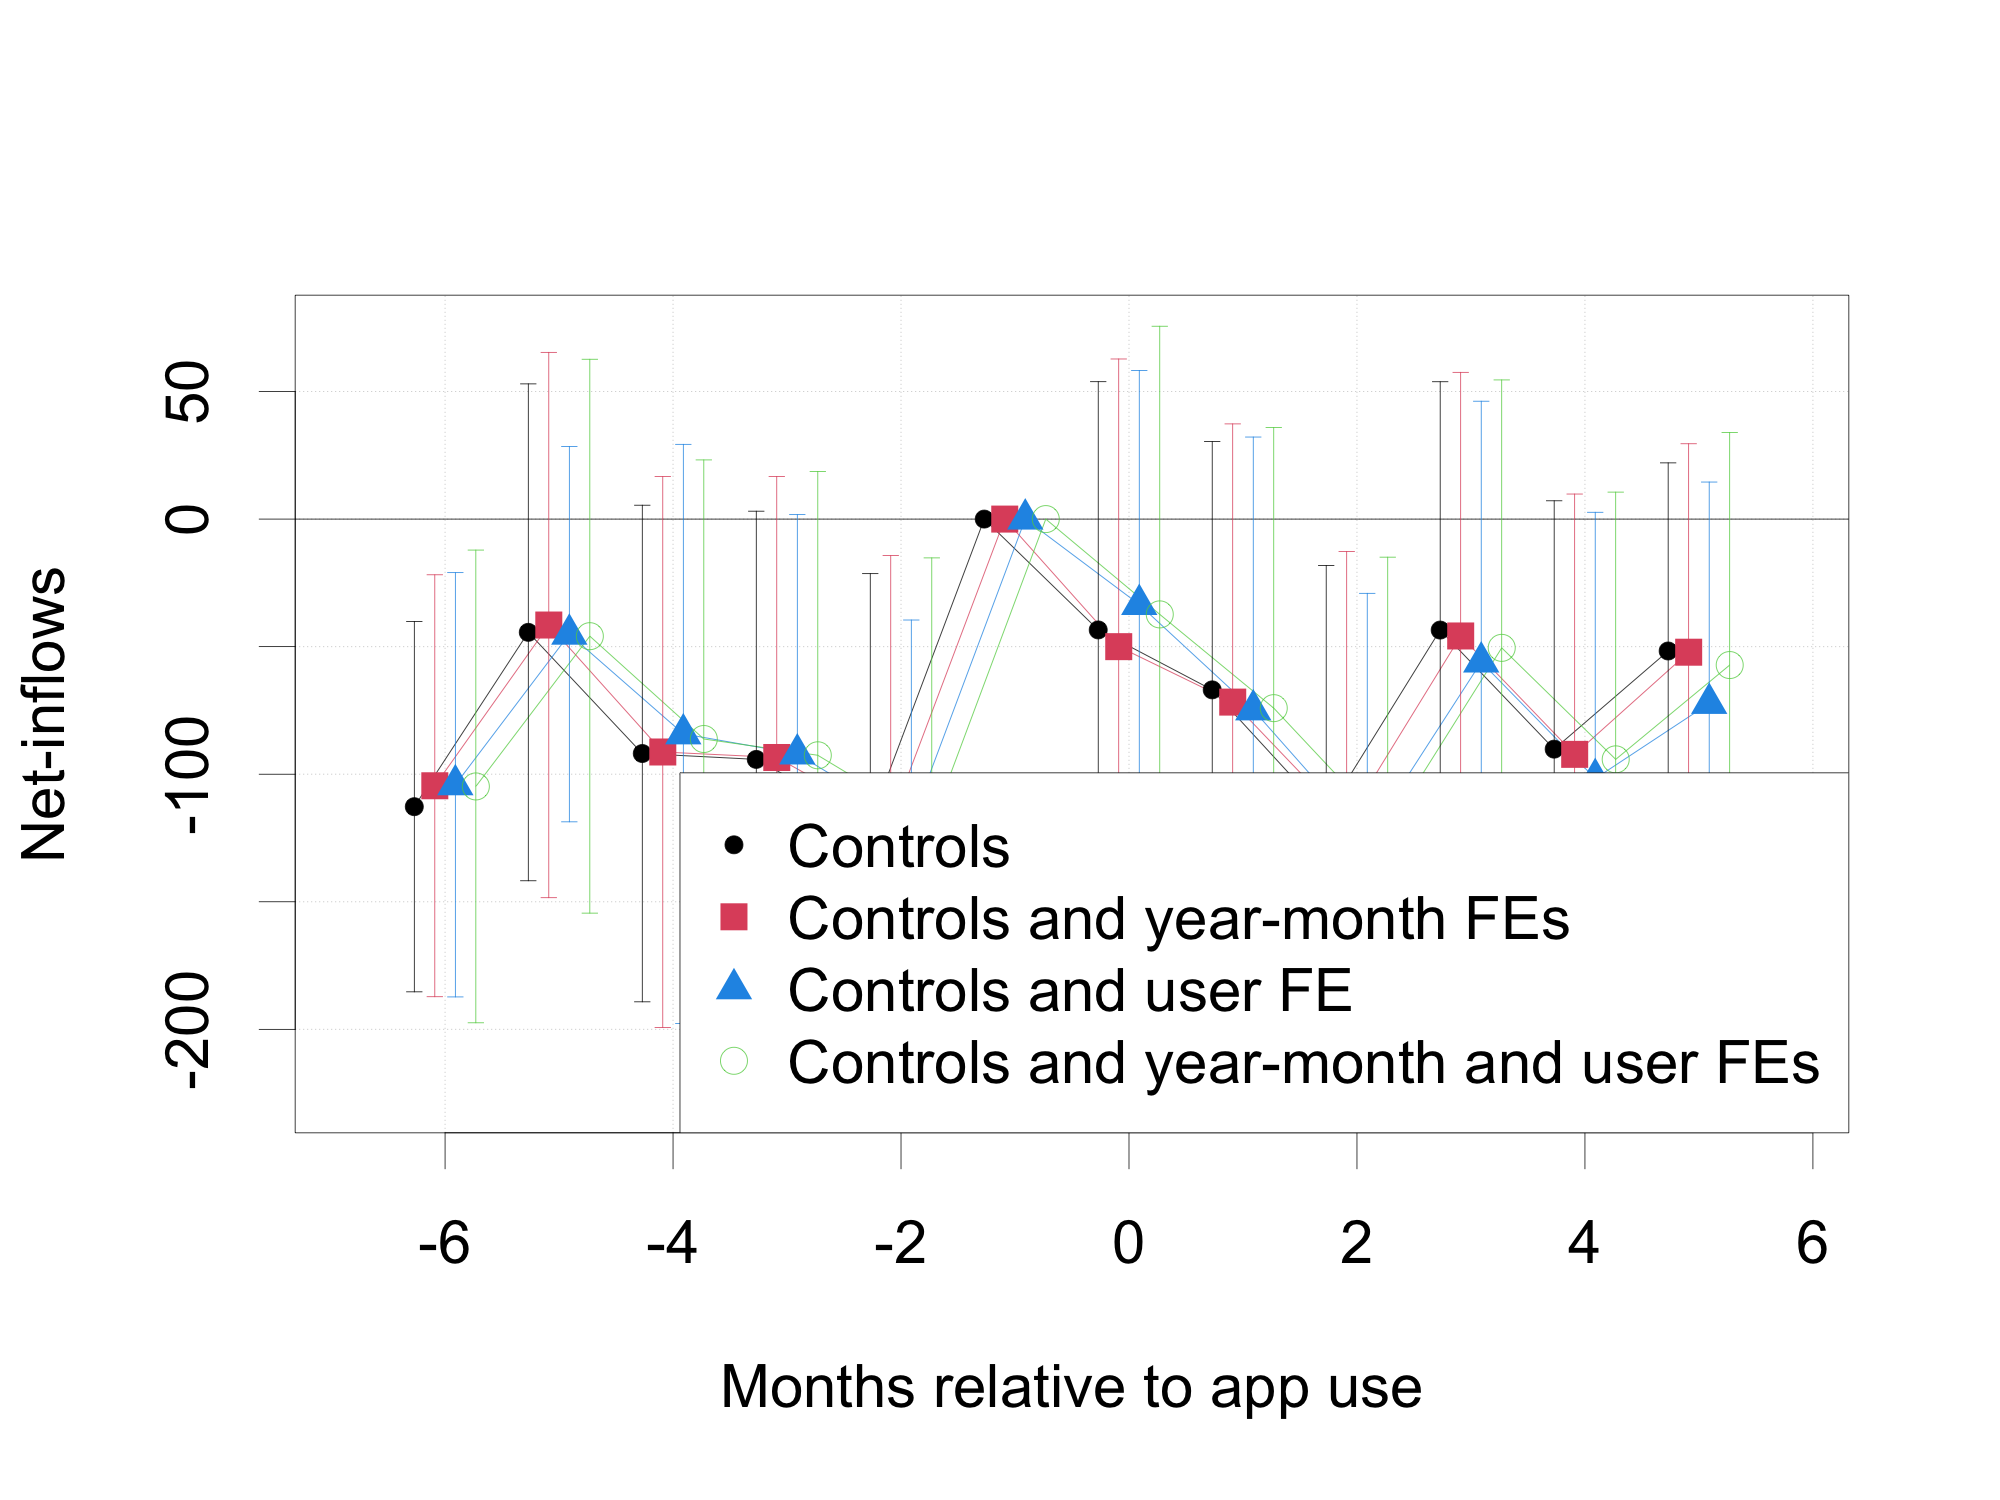
\includegraphics[width=.7\textwidth]{\figdir/netflows_alt.png}
\end{figure}


\begin{table}[htbp]
   \centering
   \tiny
   \begin{threeparttable}[b]
      \caption{\label{tab:netflows_alt} Alternative model specifications}
      \begin{tabular}{lcccc}
         \tabularnewline \midrule \midrule
         Dependent Variable: & \multicolumn{4}{c}{Net-inflows}\\
         Model:                            & (1)               & (2)               & (3)               & (4)\\  
         \midrule
         \emph{Variables}\\
         Months relative to app use $=$ -6 & -112.73$^{***}$   & -104.53$^{**}$    & -104.14$^{**}$    & -104.79$^{**}$\\   
                                           & [-185.30; -40.15] & [-187.23; -21.82] & [-189.54; -18.75] & [-197.45; -12.13]\\   
         Months relative to app use $=$ -5 & -44.39            & -41.53            & -45.12            & -45.90\\   
                                           & [-141.77; 52.99]  & [-148.42; 65.37]  & [-120.66; 30.41]  & [-154.47; 62.67]\\   
         Months relative to app use $=$ -4 & -91.89$^{*}$      & -91.29$^{*}$      & -84.19            & -86.20\\   
                                           & [-189.22; 5.44]   & [-199.28; 16.69]  & [-200.74; 32.37]  & [-195.61; 23.21]\\   
         Months relative to app use $=$ -3 & -94.20$^{*}$      & -93.45$^{*}$      & -92.07$^{*}$      & -92.58\\   
                                           & [-191.50; 3.10]   & [-203.59; 16.70]  & [-188.41; 4.27]   & [-203.84; 18.67]\\   
         Months relative to app use $=$ -2 & -118.68$^{**}$    & -118.36$^{**}$    & -119.19$^{***}$   & -119.53$^{**}$\\   
                                           & [-215.98; -21.39] & [-222.44; -14.29] & [-200.97; -37.41] & [-223.87; -15.19]\\   
         Months relative to app use $=$ 0  & -43.44            & -50.00            & -33.48            & -37.36\\   
                                           & [-140.74; 53.85]  & [-162.78; 62.77]  & [-127.72; 60.75]  & [-150.33; 75.61]\\   
         Months relative to app use $=$ 1  & -66.94            & -71.74            & -74.79            & -74.11\\   
                                           & [-164.24; 30.37]  & [-180.80; 37.33]  & [-184.62; 35.05]  & [-184.14; 35.92]\\   
         Months relative to app use $=$ 2  & -115.51$^{**}$    & -118.47$^{**}$    & -125.25$^{**}$    & -121.66$^{**}$\\   
                                           & [-212.82; -18.19] & [-224.24; -12.70] & [-224.00; -26.50] & [-228.41; -14.90]\\   
         Months relative to app use $=$ 3  & -43.50            & -45.81            & -56.03            & -50.48\\   
                                           & [-140.83; 53.83]  & [-149.17; 57.54]  & [-161.02; 48.97]  & [-155.51; 54.56]\\   
         Months relative to app use $=$ 4  & -90.18$^{*}$      & -92.22$^{*}$      & -101.71$^{*}$     & -94.18$^{*}$\\   
                                           & [-187.52; 7.17]   & [-194.27; 9.84]   & [-208.92; 5.49]   & [-198.96; 10.59]\\   
         Months relative to app use $=$ 5  & -51.70            & -52.18            & -72.25            & -57.21\\   
                                           & [-125.43; 22.03]  & [-133.90; 29.54]  & [-161.36; 16.86]  & [-148.40; 33.97]\\   
         Month income                      & 0.07$^{***}$      & 0.07$^{***}$      & 0.07$^{***}$      & 0.08$^{***}$\\   
                                           & [0.06; 0.08]      & [0.05; 0.10]      & [0.05; 0.09]      & [0.05; 0.10]\\   
         Month spend                       & -0.12$^{***}$     & -0.16$^{***}$     & -0.12$^{***}$     & -0.16$^{***}$\\   
                                           & [-0.13; -0.11]    & [-0.19; -0.14]    & [-0.14; -0.10]    & [-0.19; -0.14]\\   
         Active accounts                   & 38.47$^{***}$     & 72.54$^{***}$     & 37.00$^{***}$     & 72.05$^{***}$\\   
                                           & [30.62; 46.31]    & [56.98; 88.10]    & [24.59; 51.40]    & [56.26; 87.84]\\   
         Intercept                         & 95.97$^{**}$      &                   &                   &   \\   
                                           & [20.52; 171.42]   &                   &                   &   \\   
         \midrule
         \emph{Fixed-effects}\\
         User ID                           &                   & Yes               &                   & Yes\\  
         Year-month                        &                   &                   & Yes               & Yes\\  
         \midrule
         \emph{Fit statistics}\\
         Observations                      & 188,324           & 188,324           & 188,324           & 188,324\\  
         R$^2$                             & 0.00897           & 0.04121           & 0.00948           & 0.04170\\  
         Within R$^2$                      &                   & 0.01022           & 0.00885           & 0.01007\\  
         \midrule \midrule
         \multicolumn{5}{l}{\emph{Signif. Codes: ***: 0.01, **: 0.05, *: 0.1}}\\
      \end{tabular}
   \end{threeparttable}
\end{table}






\subsection{Subgroups}%
\label{sub:subgroups}

To analyse which groups benefit most from adopting Money Dashboard, we split
our sample by gender, generation, income quartiles, and pre-adoption savings
behaviour.

We define generations as follows: boomers were born between 1946 and 1964, Gen
X between 1965 and 1980, Millennials between 1981 and 1996, and Gen Z after
1997.\footnote{Based on age ranges provides by
    \href{https://www.beresfordresearch.com/age-range-by-generation/}{Beresford
Research}.}

Subgroup analysis: same Fig an Tab as in main analysis, but with line for each
subgroup. One figure for each of: gender, generations, income terciles,
per-adoption average savings tercile (inspired by \citet{carlin2017fintech},
see Fig 5 and Table 4).

See also section 6 in \citet{gargano2021goal}



\section{Results}%
\label{sec:results}

Main results: Figure and associated table akin to sakaguchi2022default Figure 2
and Table 6.

\subsection{Descriptive analysis}%
\label{sub:descriptive_analysis}

\subsection{Difference-in-difference analysis}%
\label{sub:difference_in_difference_analysis}

\subsection{Subgroups}%
\label{sub:subgroups}

To analyse which groups benefit most from adopting Money Dashboard, we split
our sample by gender, generation, income quartiles, and pre-adoption savings
behaviour.

We define generations as follows: boomers were born between 1946 and 1964, Gen
X between 1965 and 1980, Millennials between 1981 and 1996, and Gen Z after
1997.\footnote{Based on age ranges provides by
    \href{https://www.beresfordresearch.com/age-range-by-generation/}{Beresford
Research}.}

Subgroup analysis: same Fig an Tab as in main analysis, but with line for each
subgroup. One figure for each of: gender, generations, income terciles,
per-adoption average savings tercile (inspired by \citet{carlin2017fintech},
see Fig 5 and Table 4).

% % !TEX root = ../eval.tex

\section{Discussion}%
\label{sec:discussion}

Limitations:
\begin{itemize}
    \item Can't say whether increase in savings was achieved by going into
        debt elsewhere

    \item Limitations: We have more data for users that signed up later. So average user in
        the study is not the average MDB user. If time of signup is mainly
        driven by financial savyness, then study sample is closer to overall
        population than MDB sample (if we rank groups as early joiners > late
        joiners > never joiners in terms of financial sophistication). If,
        however, signup reflects something like openness to newness, then it's
        not necessarily correlated with financial savyness. Either way, we
        might ignore it for now. We could test whether behaviour differs
        between early or late adopters, but that doesn't seem important enough.

\end{itemize}

\section{Discussion}%
\label{sec:discussion}


\newpage
\printbibliography
\newpage

% % !TEX root = ../eval.tex

\section{Unbalanced aggregation}%
\label{sec:unbalanced_aggregation}

The baseline specification relies on a panel balanced in event time and
thus only includes users that have been exposed to treatment for at least 5
periods. Figure~\ref{fig:ub_comp} reproduces the baseline results in the left
panel and compares it with results based on the full sample.

As discussed in section 3.1.1 of \citet{callaway2021difference}, these two
approaches entail a trade-off. When using the full sample, the aggregated
parameters are a function of the weighted average treatment effects for each
group $l$ periods after treatment (which is what we want) as well as
compositional changes due to different groups being included for different
periods $l$ and different weights attached to these groups. While parameters
aggregated using a panel balanced in event time do not suffer from
compositional and weighting changes, but are calculated based on a smaller
number of groups.

As expected, using the full data reduces the size of the confidence intervals.
But the results are otherwise very similar.

\begin{figure}[h]
    \centering
    \caption{Balanced and unbalanced aggregation}%
    \label{fig:ub_comp}
    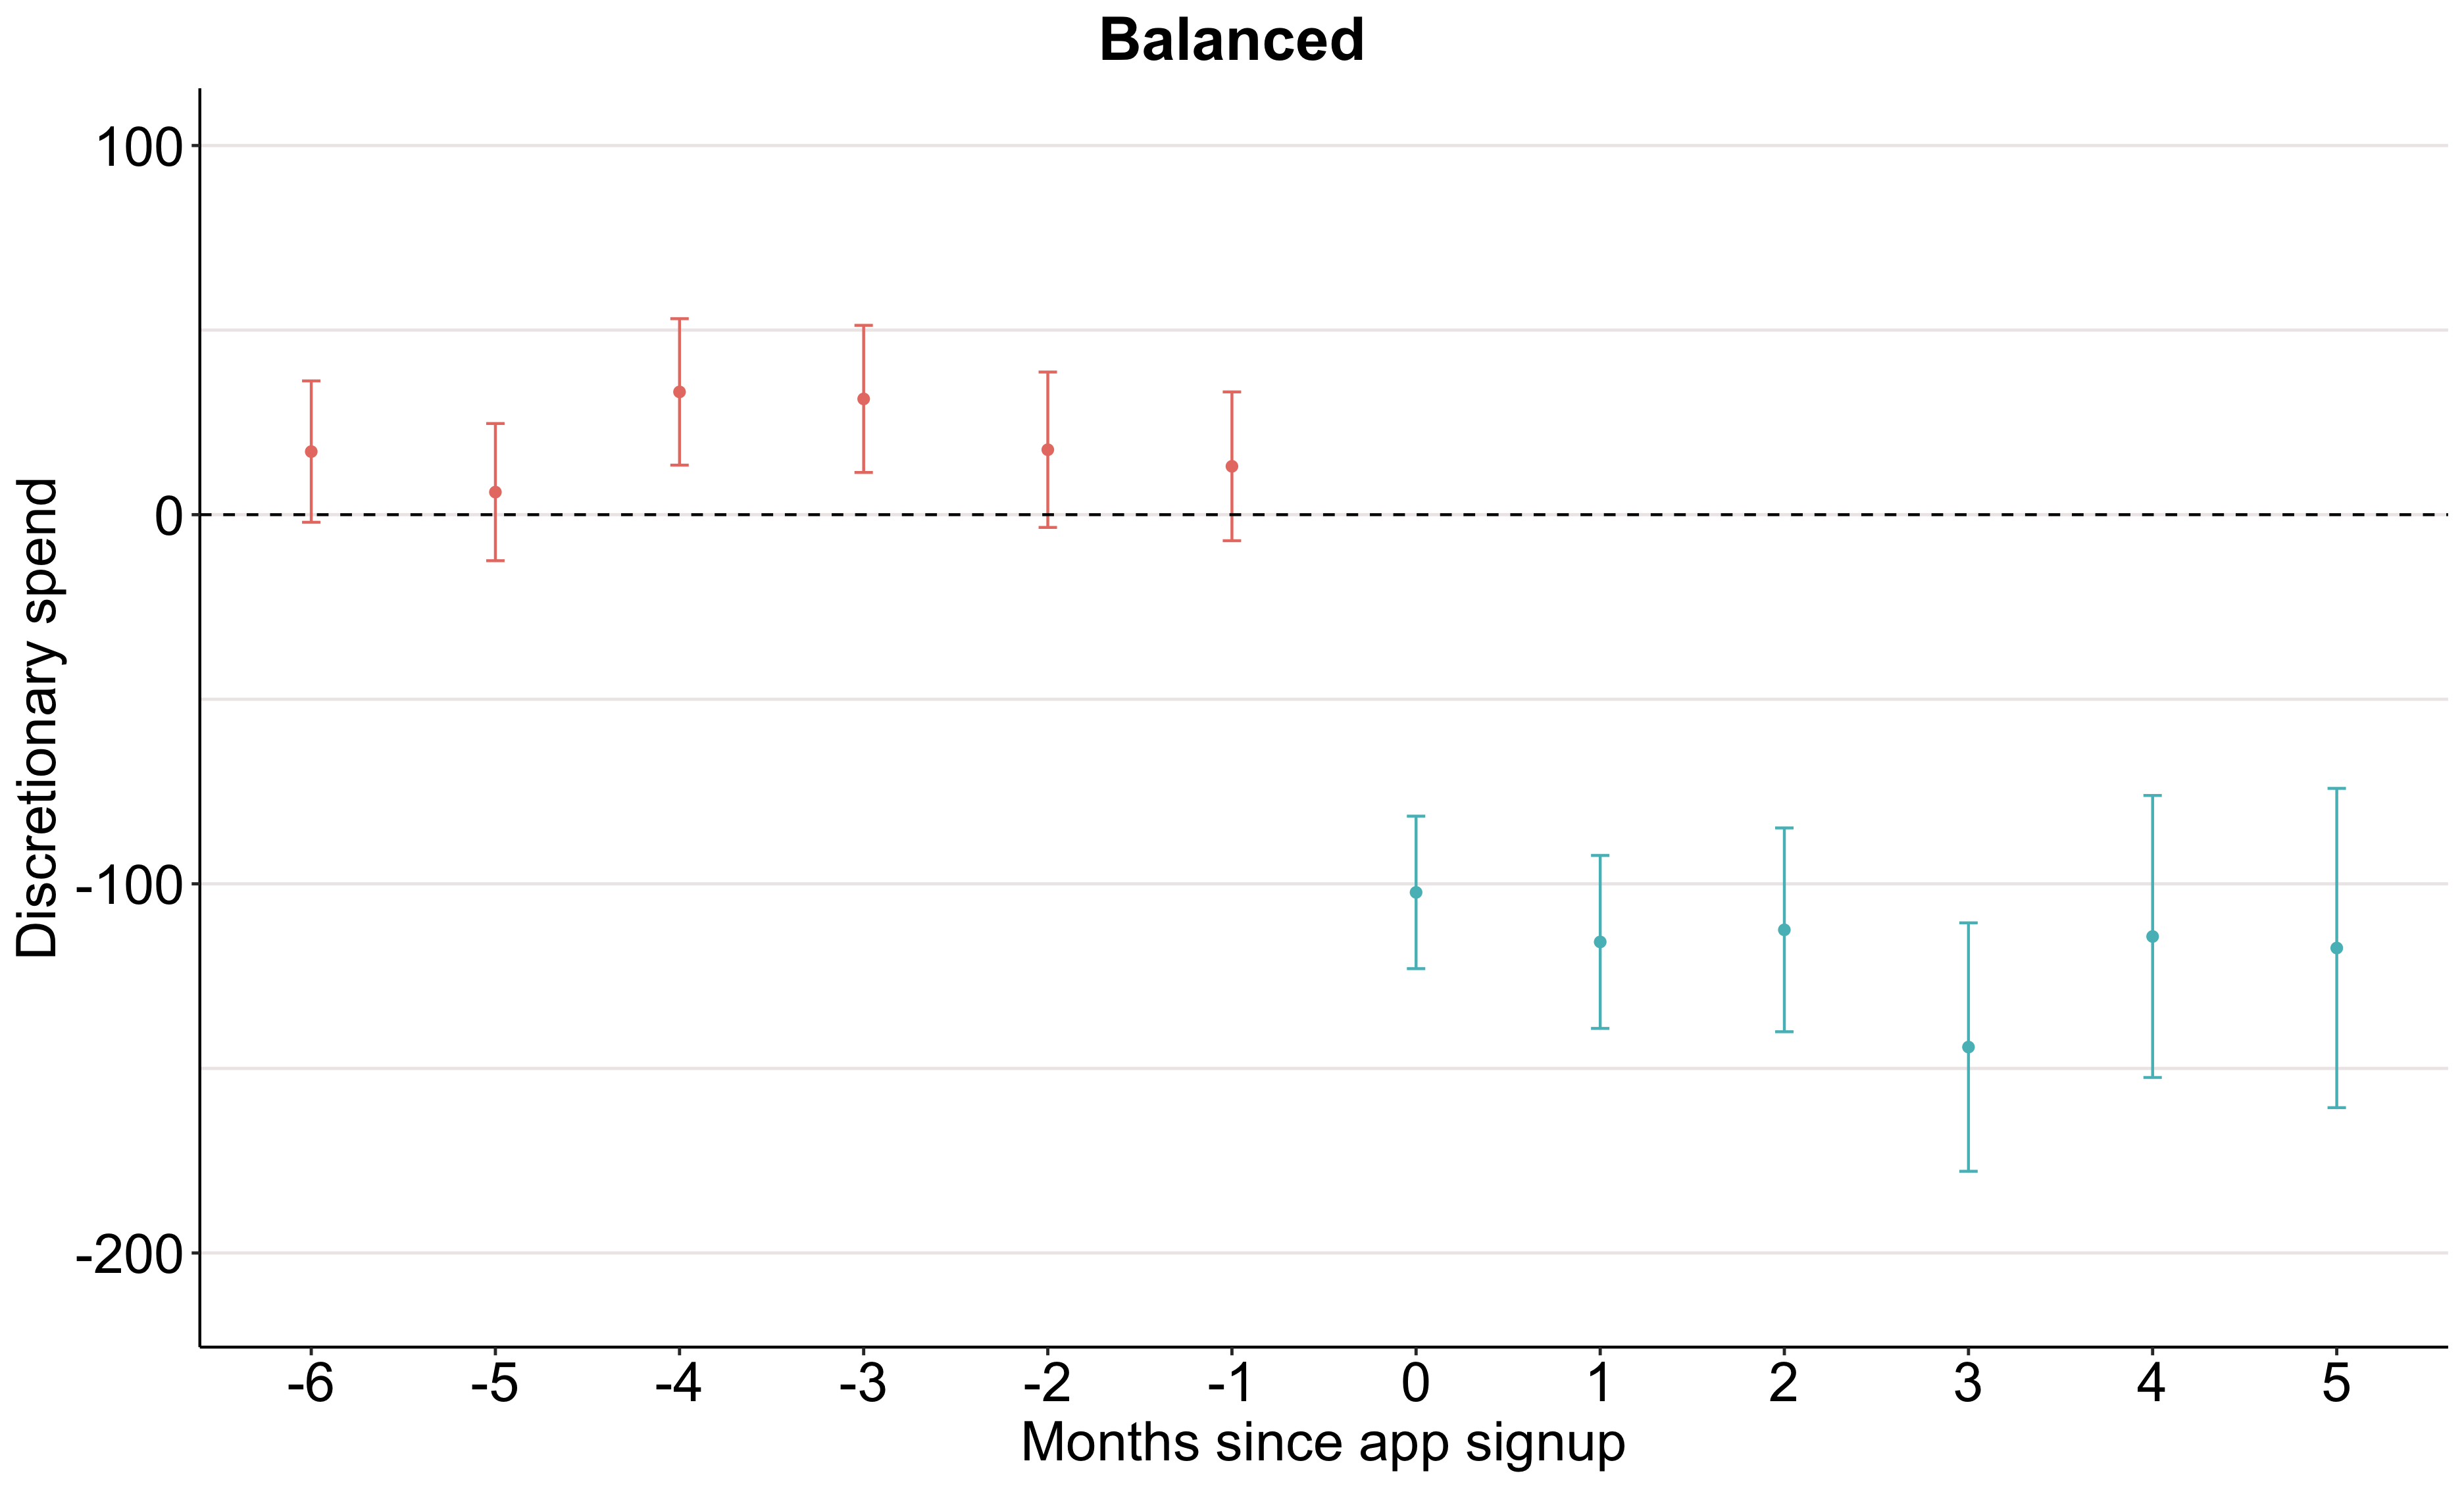
\includegraphics[width=.49\textwidth]{\figdir/dspend_cond_bal_es.png}
    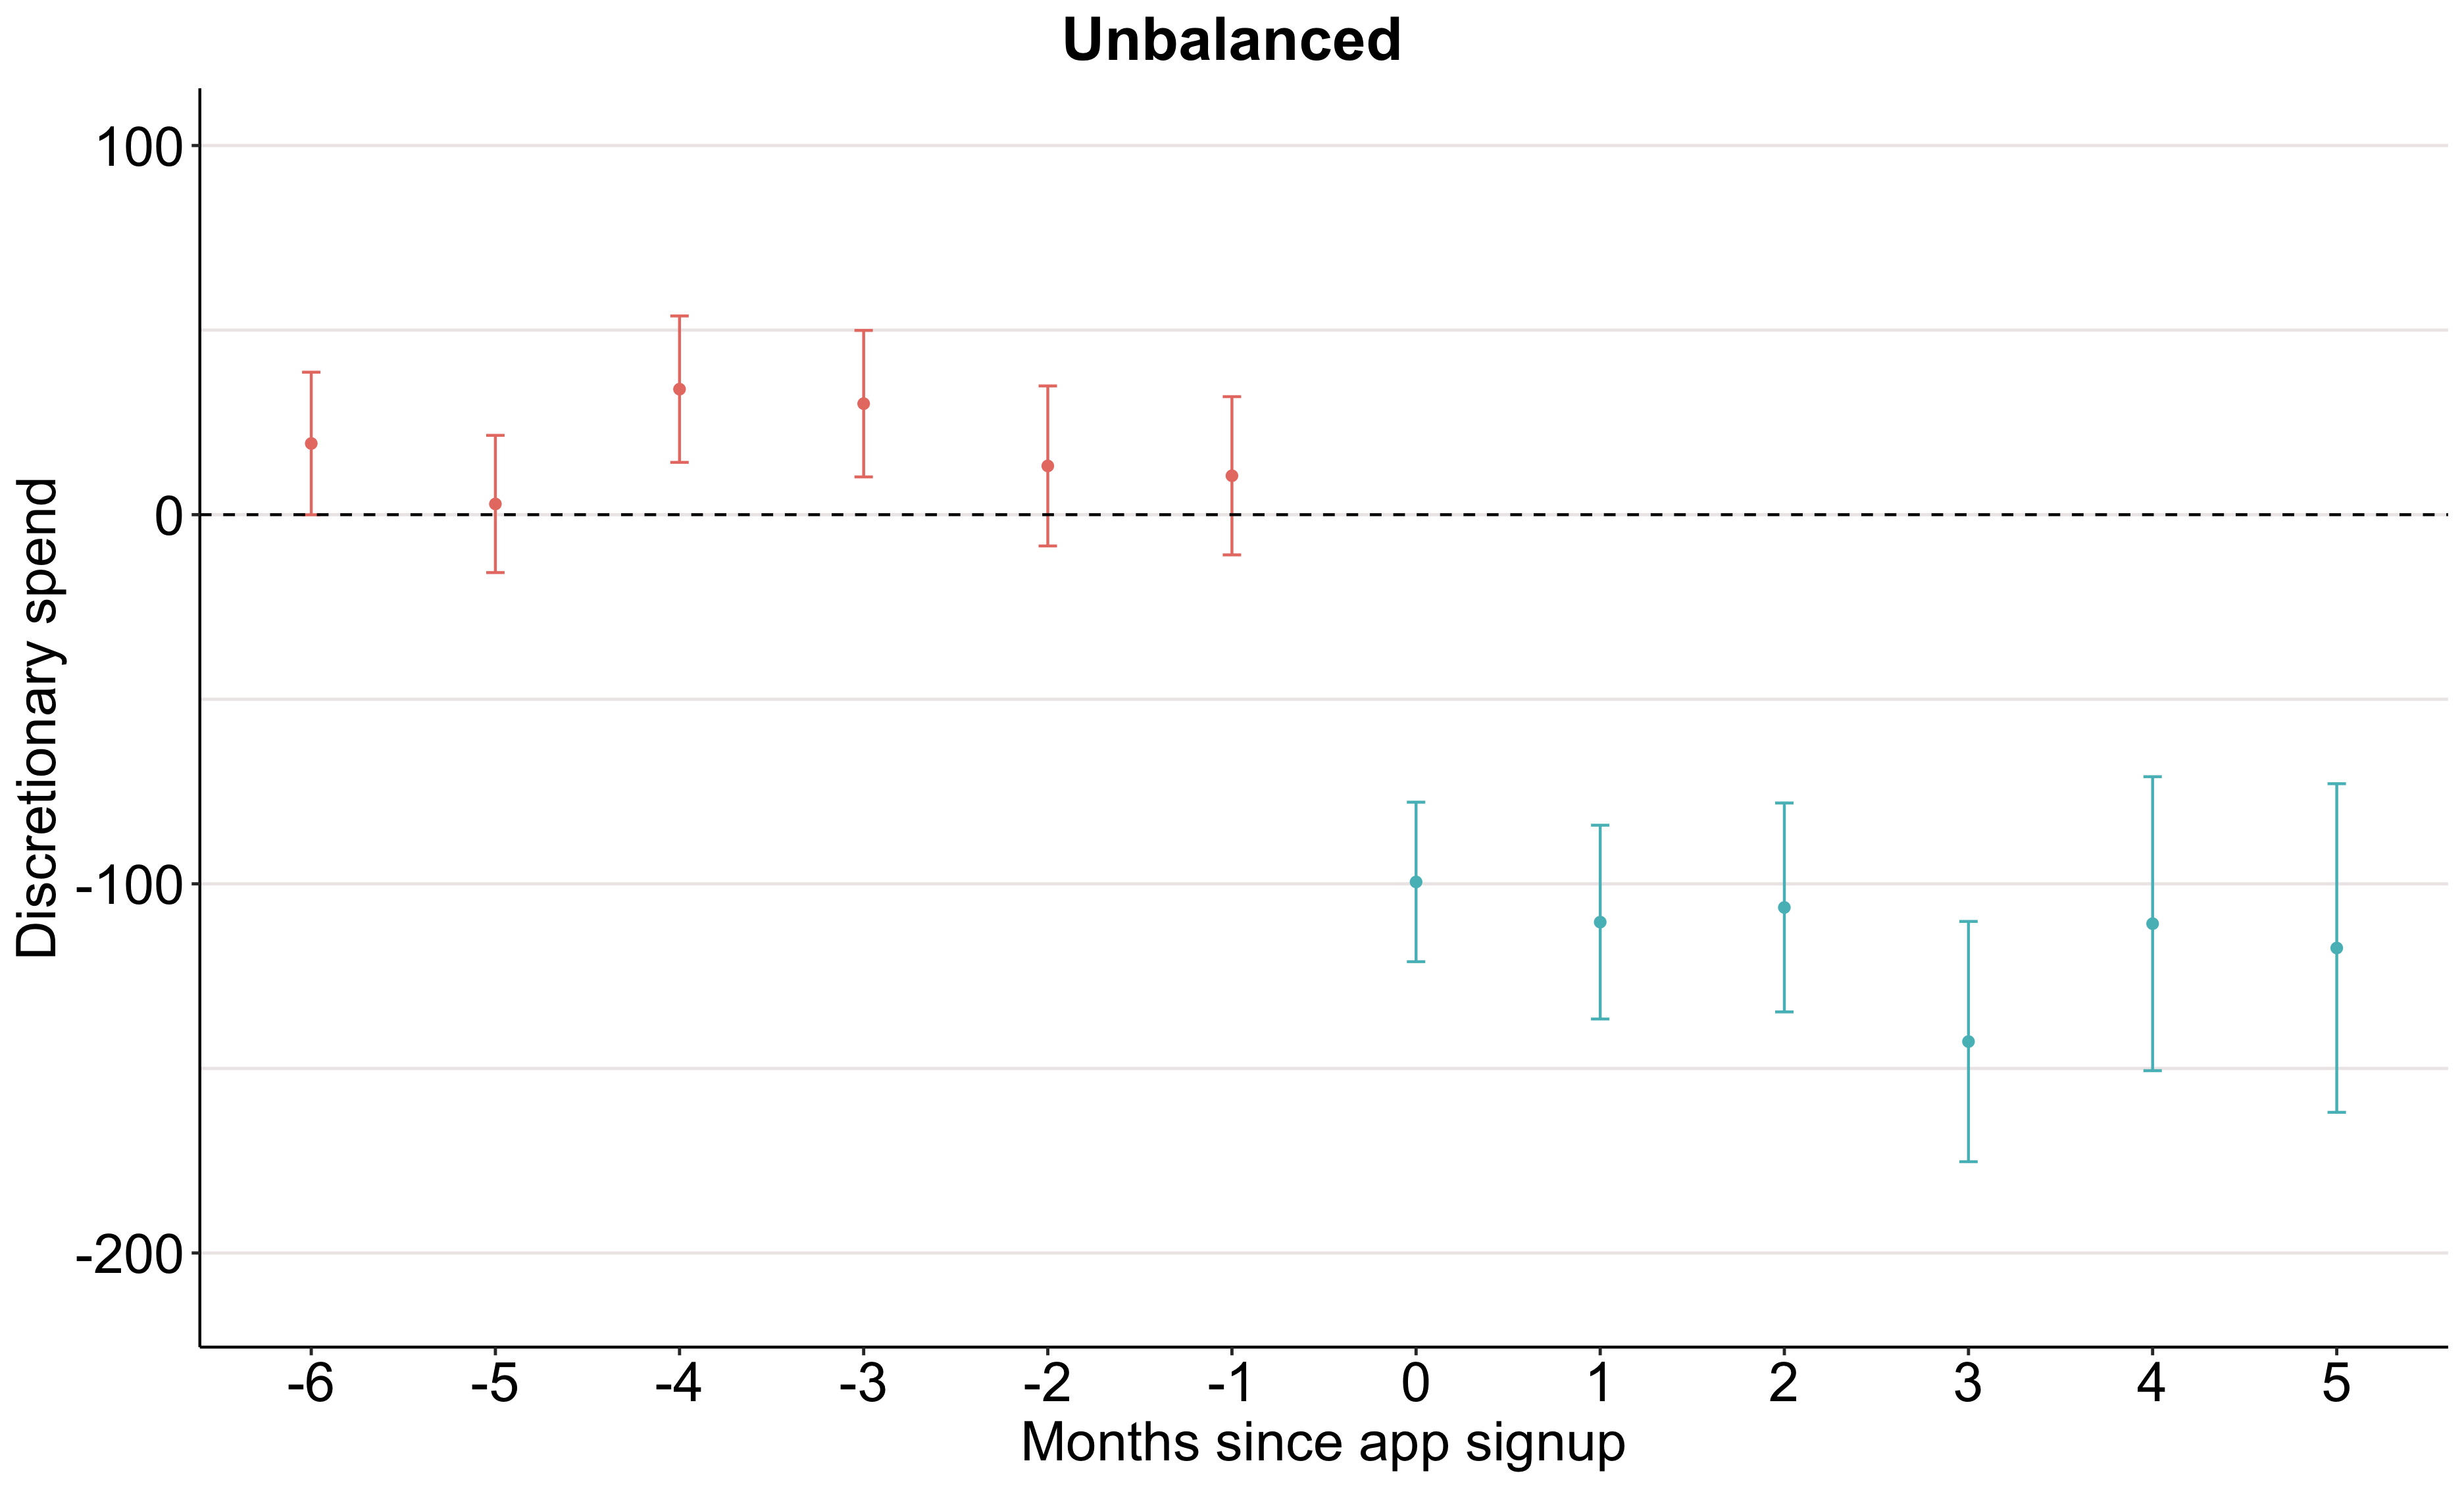
\includegraphics[width=.49\textwidth]{\figdir/dspend_cond_unbal_es.png}
    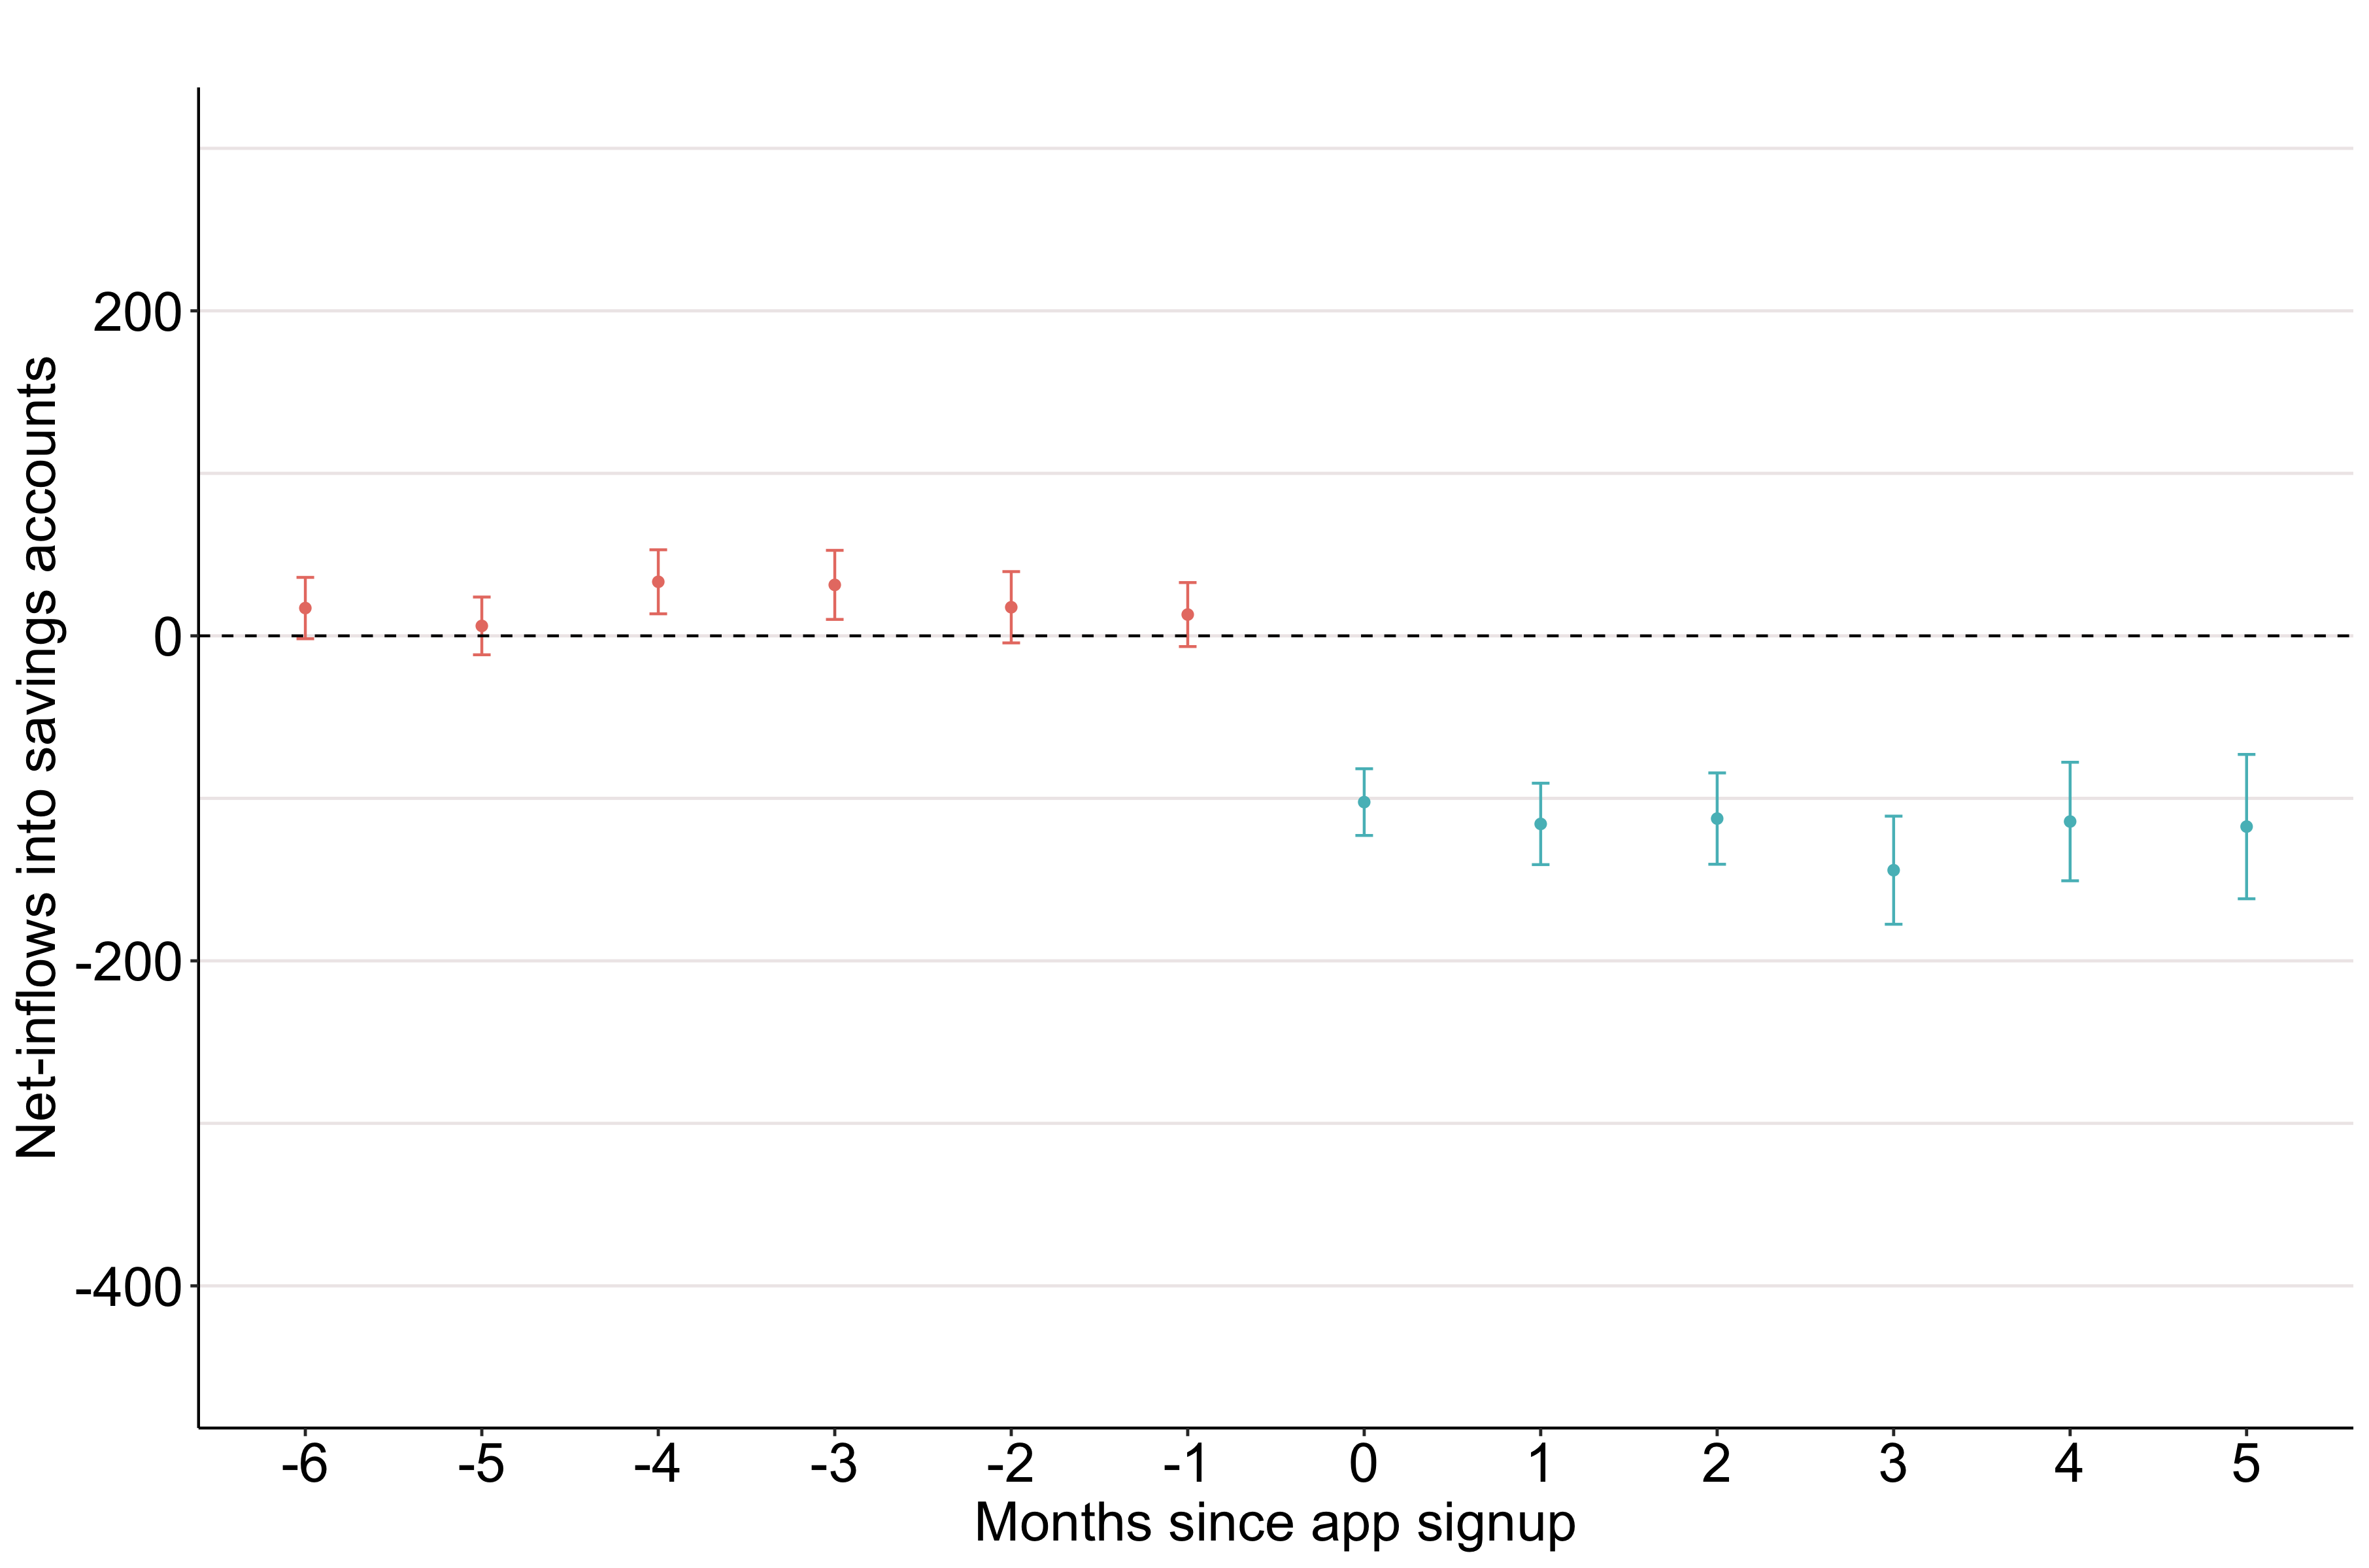
\includegraphics[width=.49\textwidth]{\figdir/netflows_cond_bal_es.png}
    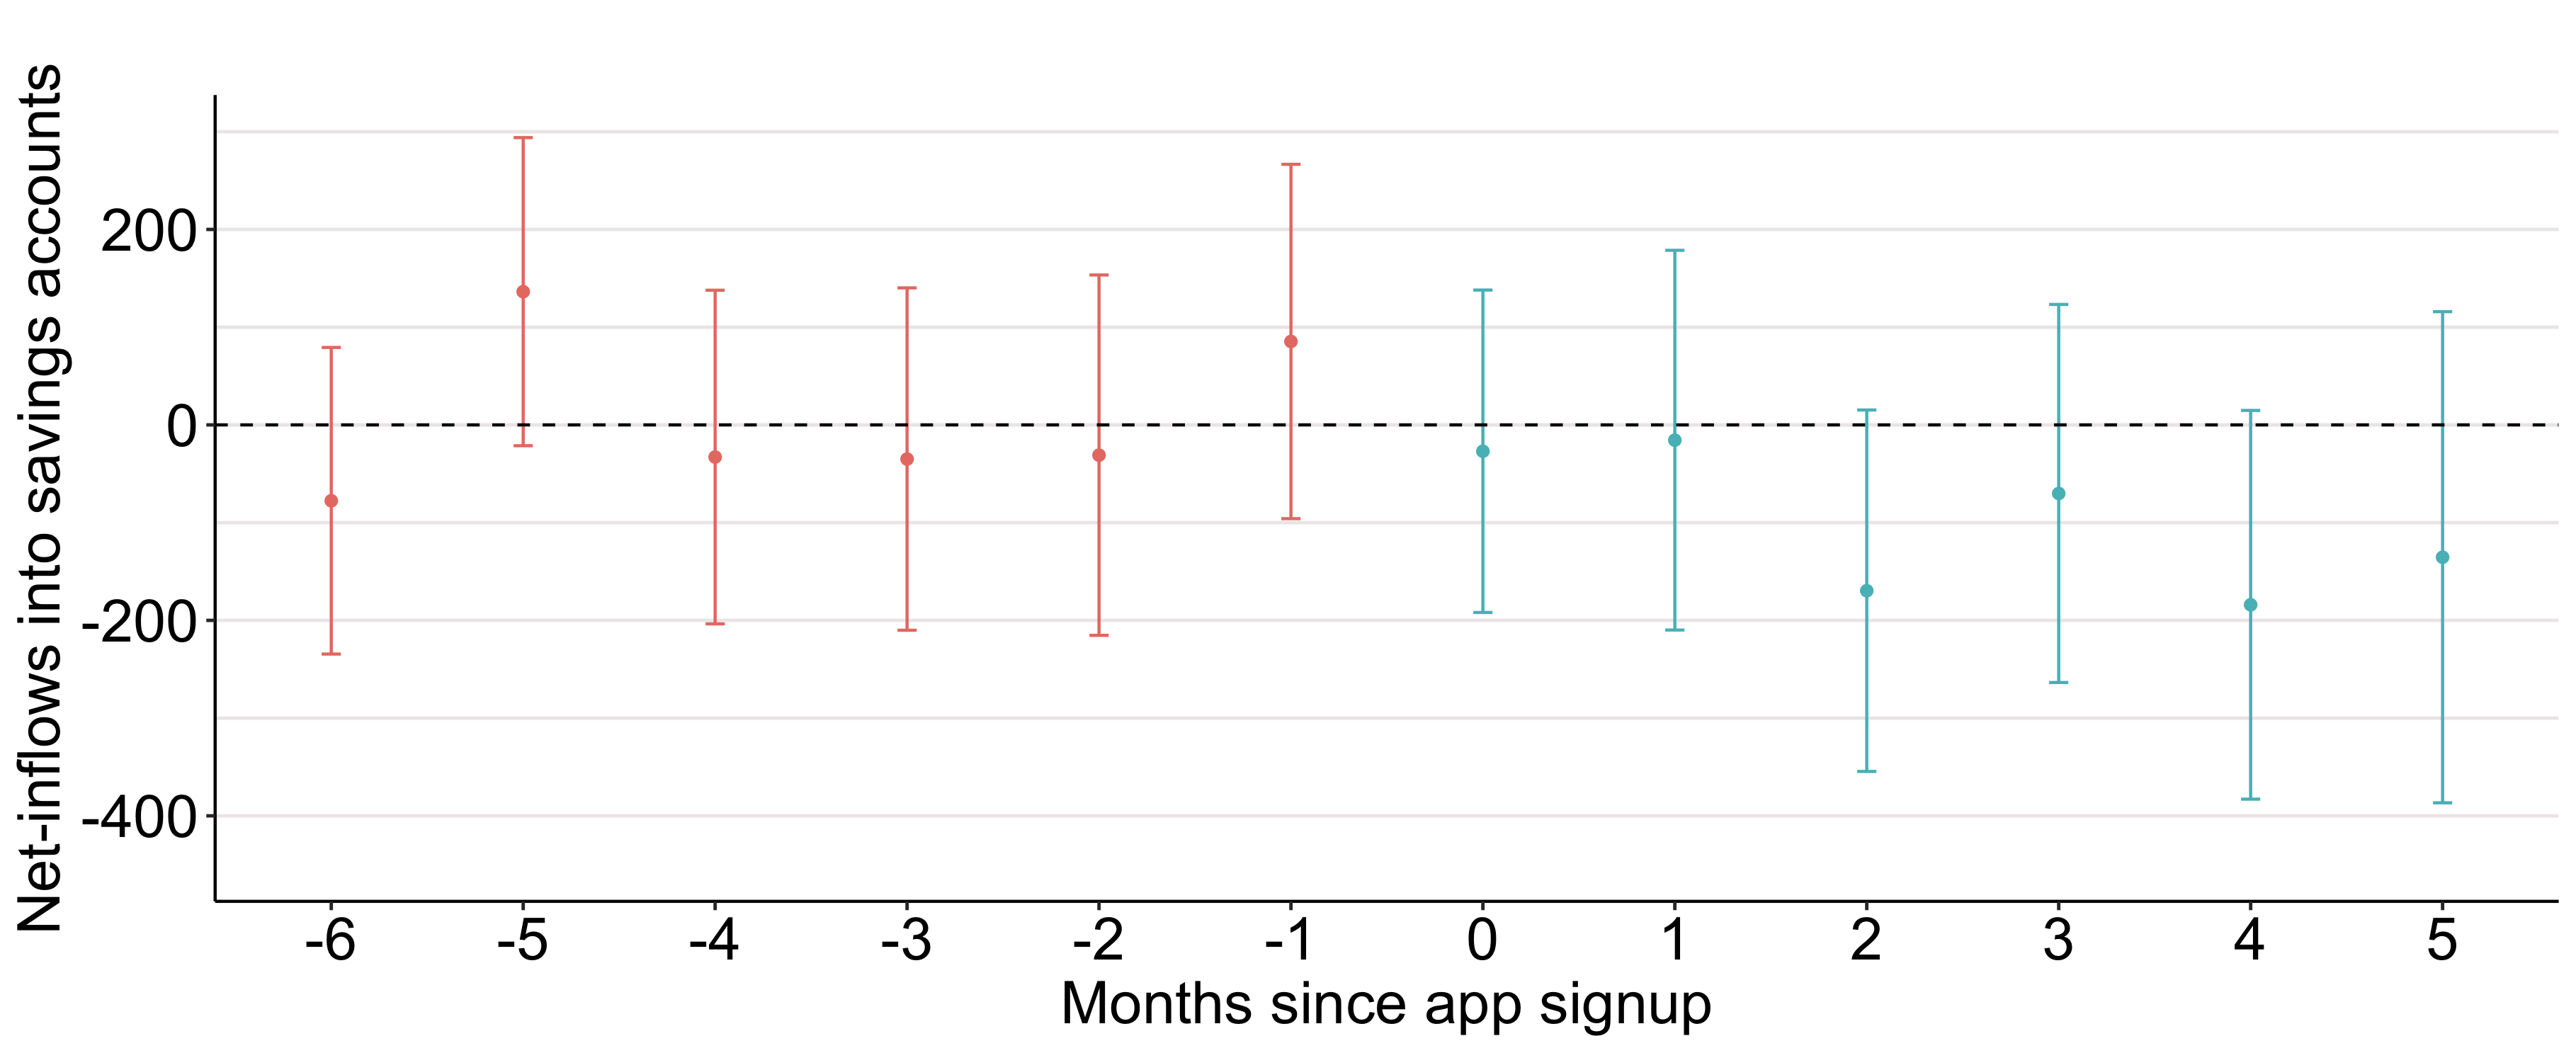
\includegraphics[width=.49\textwidth]{\figdir/netflows_cond_unbal_es.png}
    \fignote{\textwidth}{Main results based on balanced and unbalanced panels.
        Point estimates represent group-time average treatment effects
        aggregated to periods since treatment exposure, as defined in
        Section~\ref{sec:estimation}. Red lines represent point estimates and
        uniform 95\% confidence bands for pre-treatment periods allowing for
        clustering at the user level. If the null hypothesis that parallel
        trends hold in all periods is correct, these should be equal to zero.
        Blue lines provide similar information for post-treatment periods.}
\end{figure}



\section{Inflows and outflows}%
\label{sec:inflows_and_outflows}

The leftmost panel in Figure~\ref{fig:in_out_results} reproduces the results from
Figure~\ref{fig:main_results} for net-inflows into savings accounts using the
conditional parallel trends assumption for reference, and decomposes these
net-inflows into inflows (middle) and outflows (right). We can see that
net-inflows remain unchanged because both inflows and outflows remain
unchanged and not because a change in inflows if offset by a commensurate
change in outflows.

\begin{figure}[H]
    \centering
    \caption{Decomposing net-inflows into inflows and outflows}%
    \label{fig:in_out_results}
    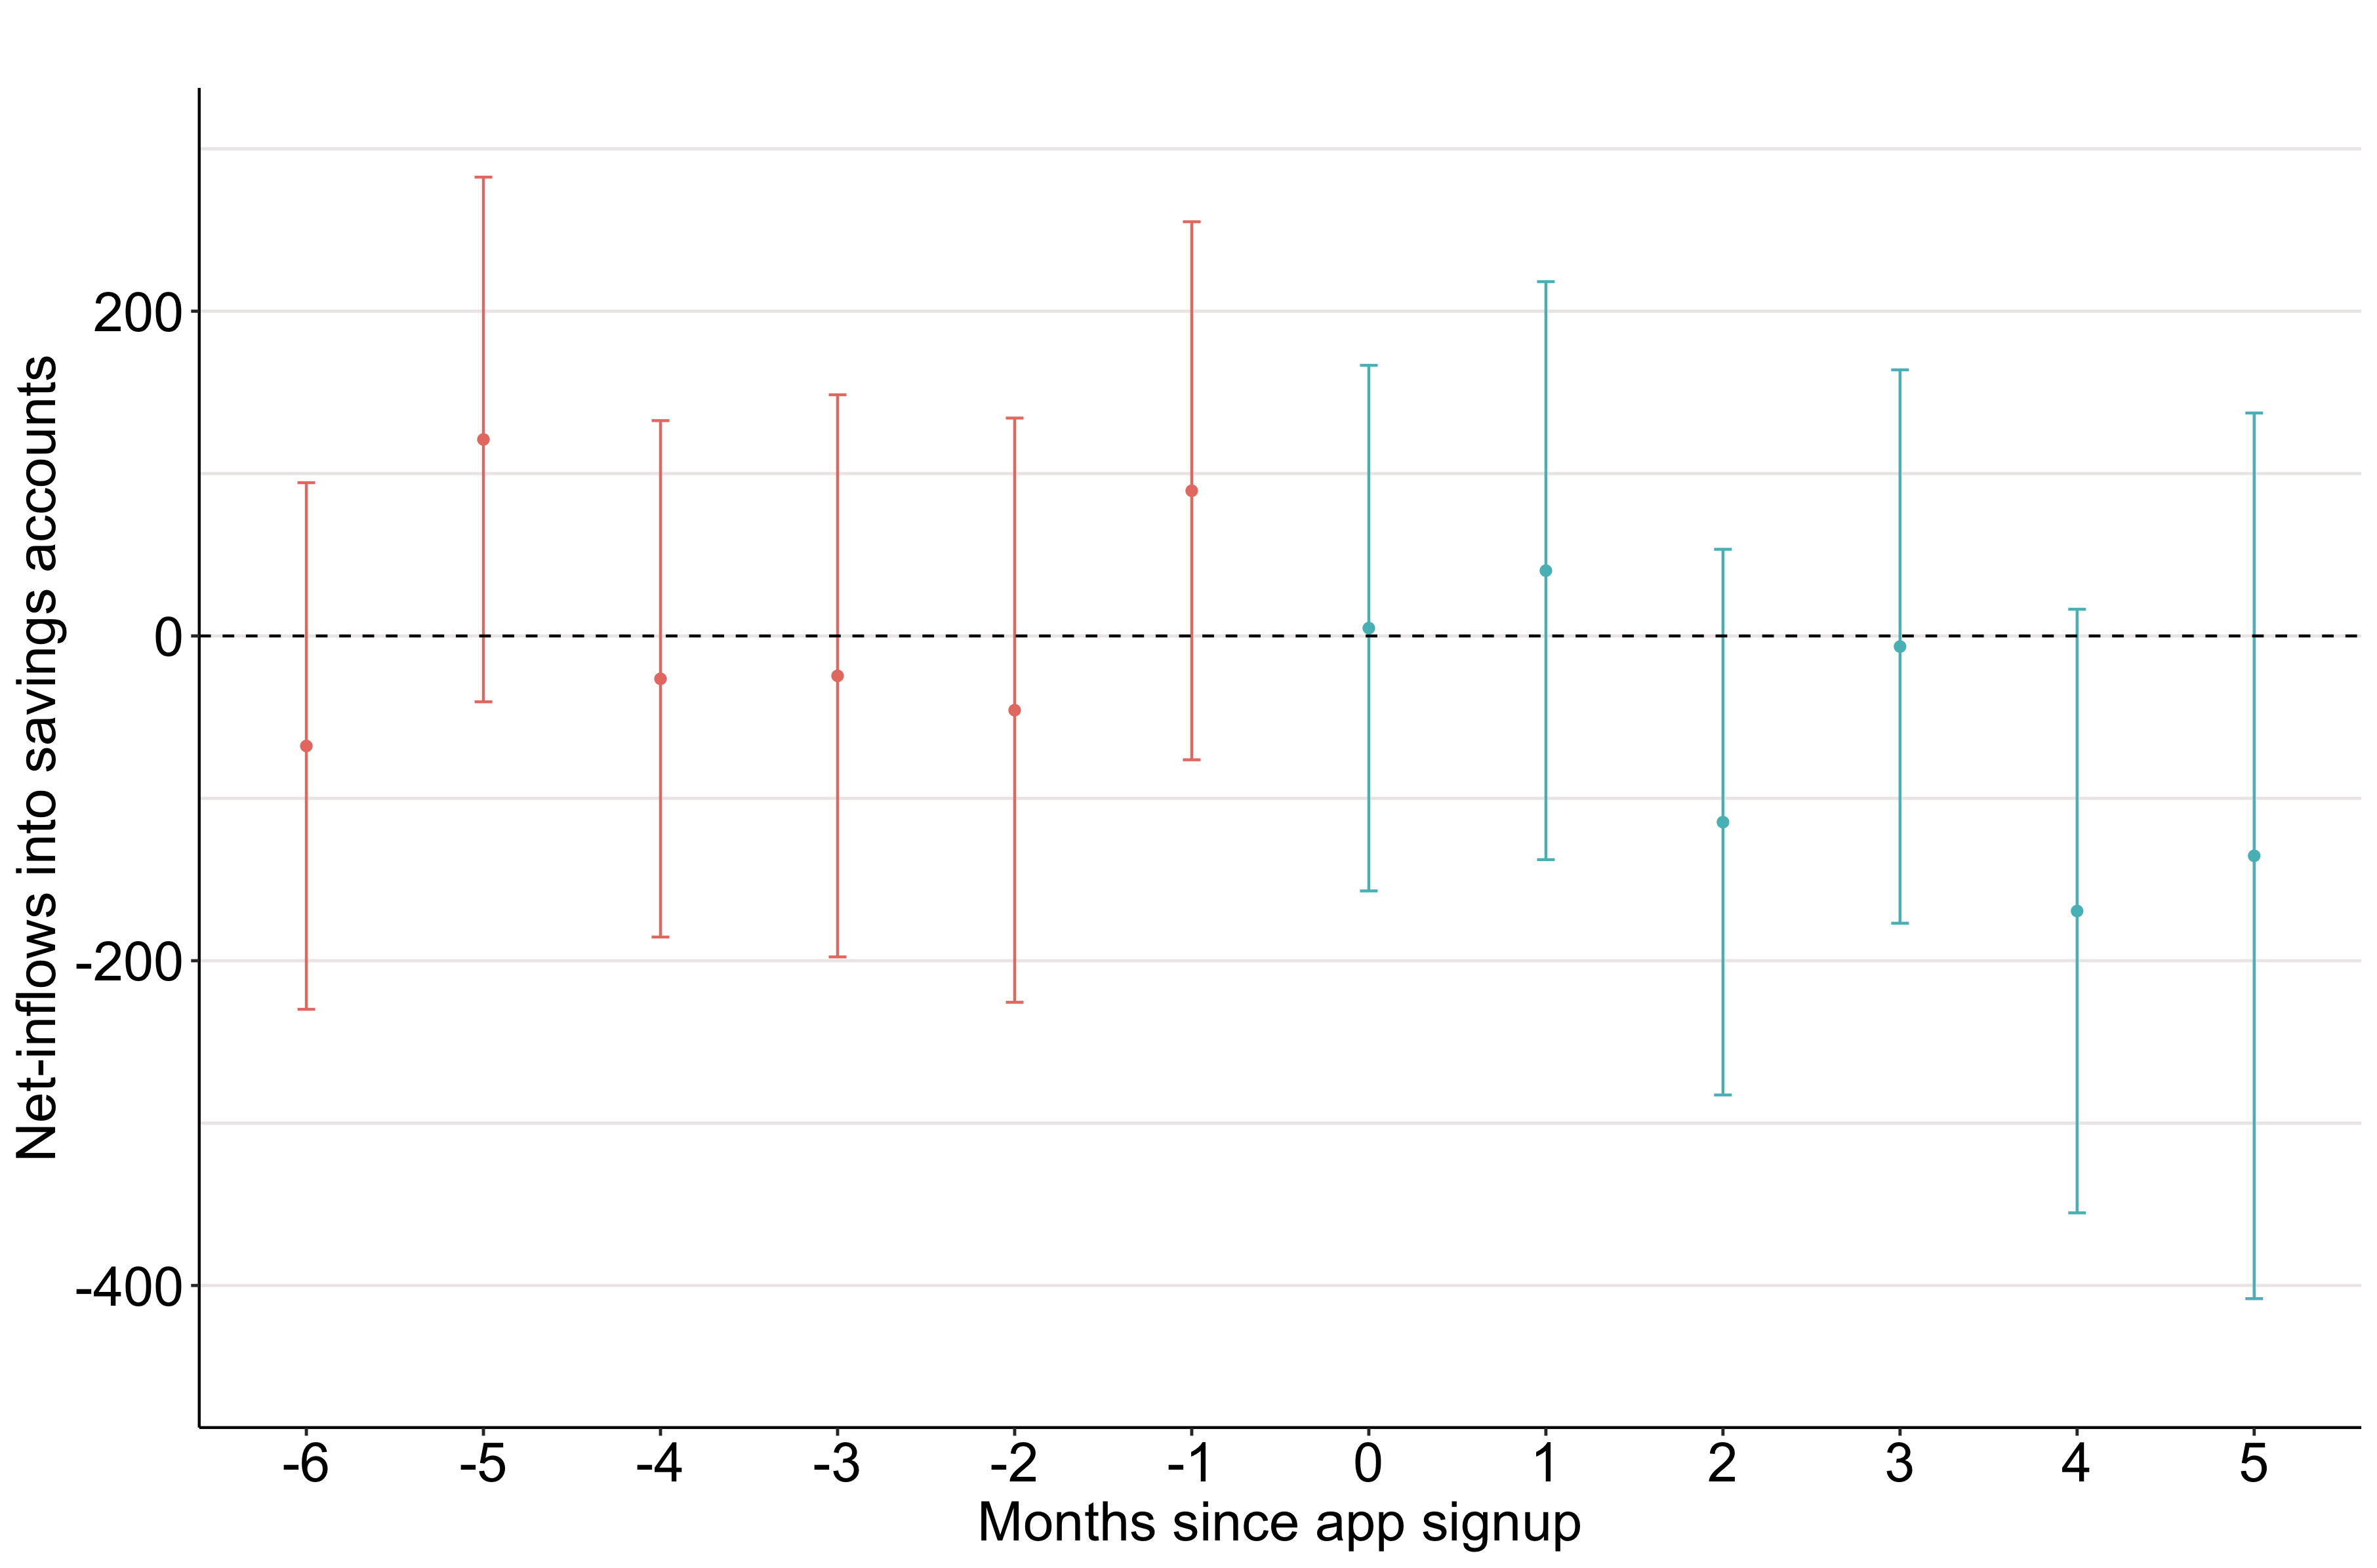
\includegraphics[width=.32\textwidth]{\figdir/netflows_cond_es.png}
    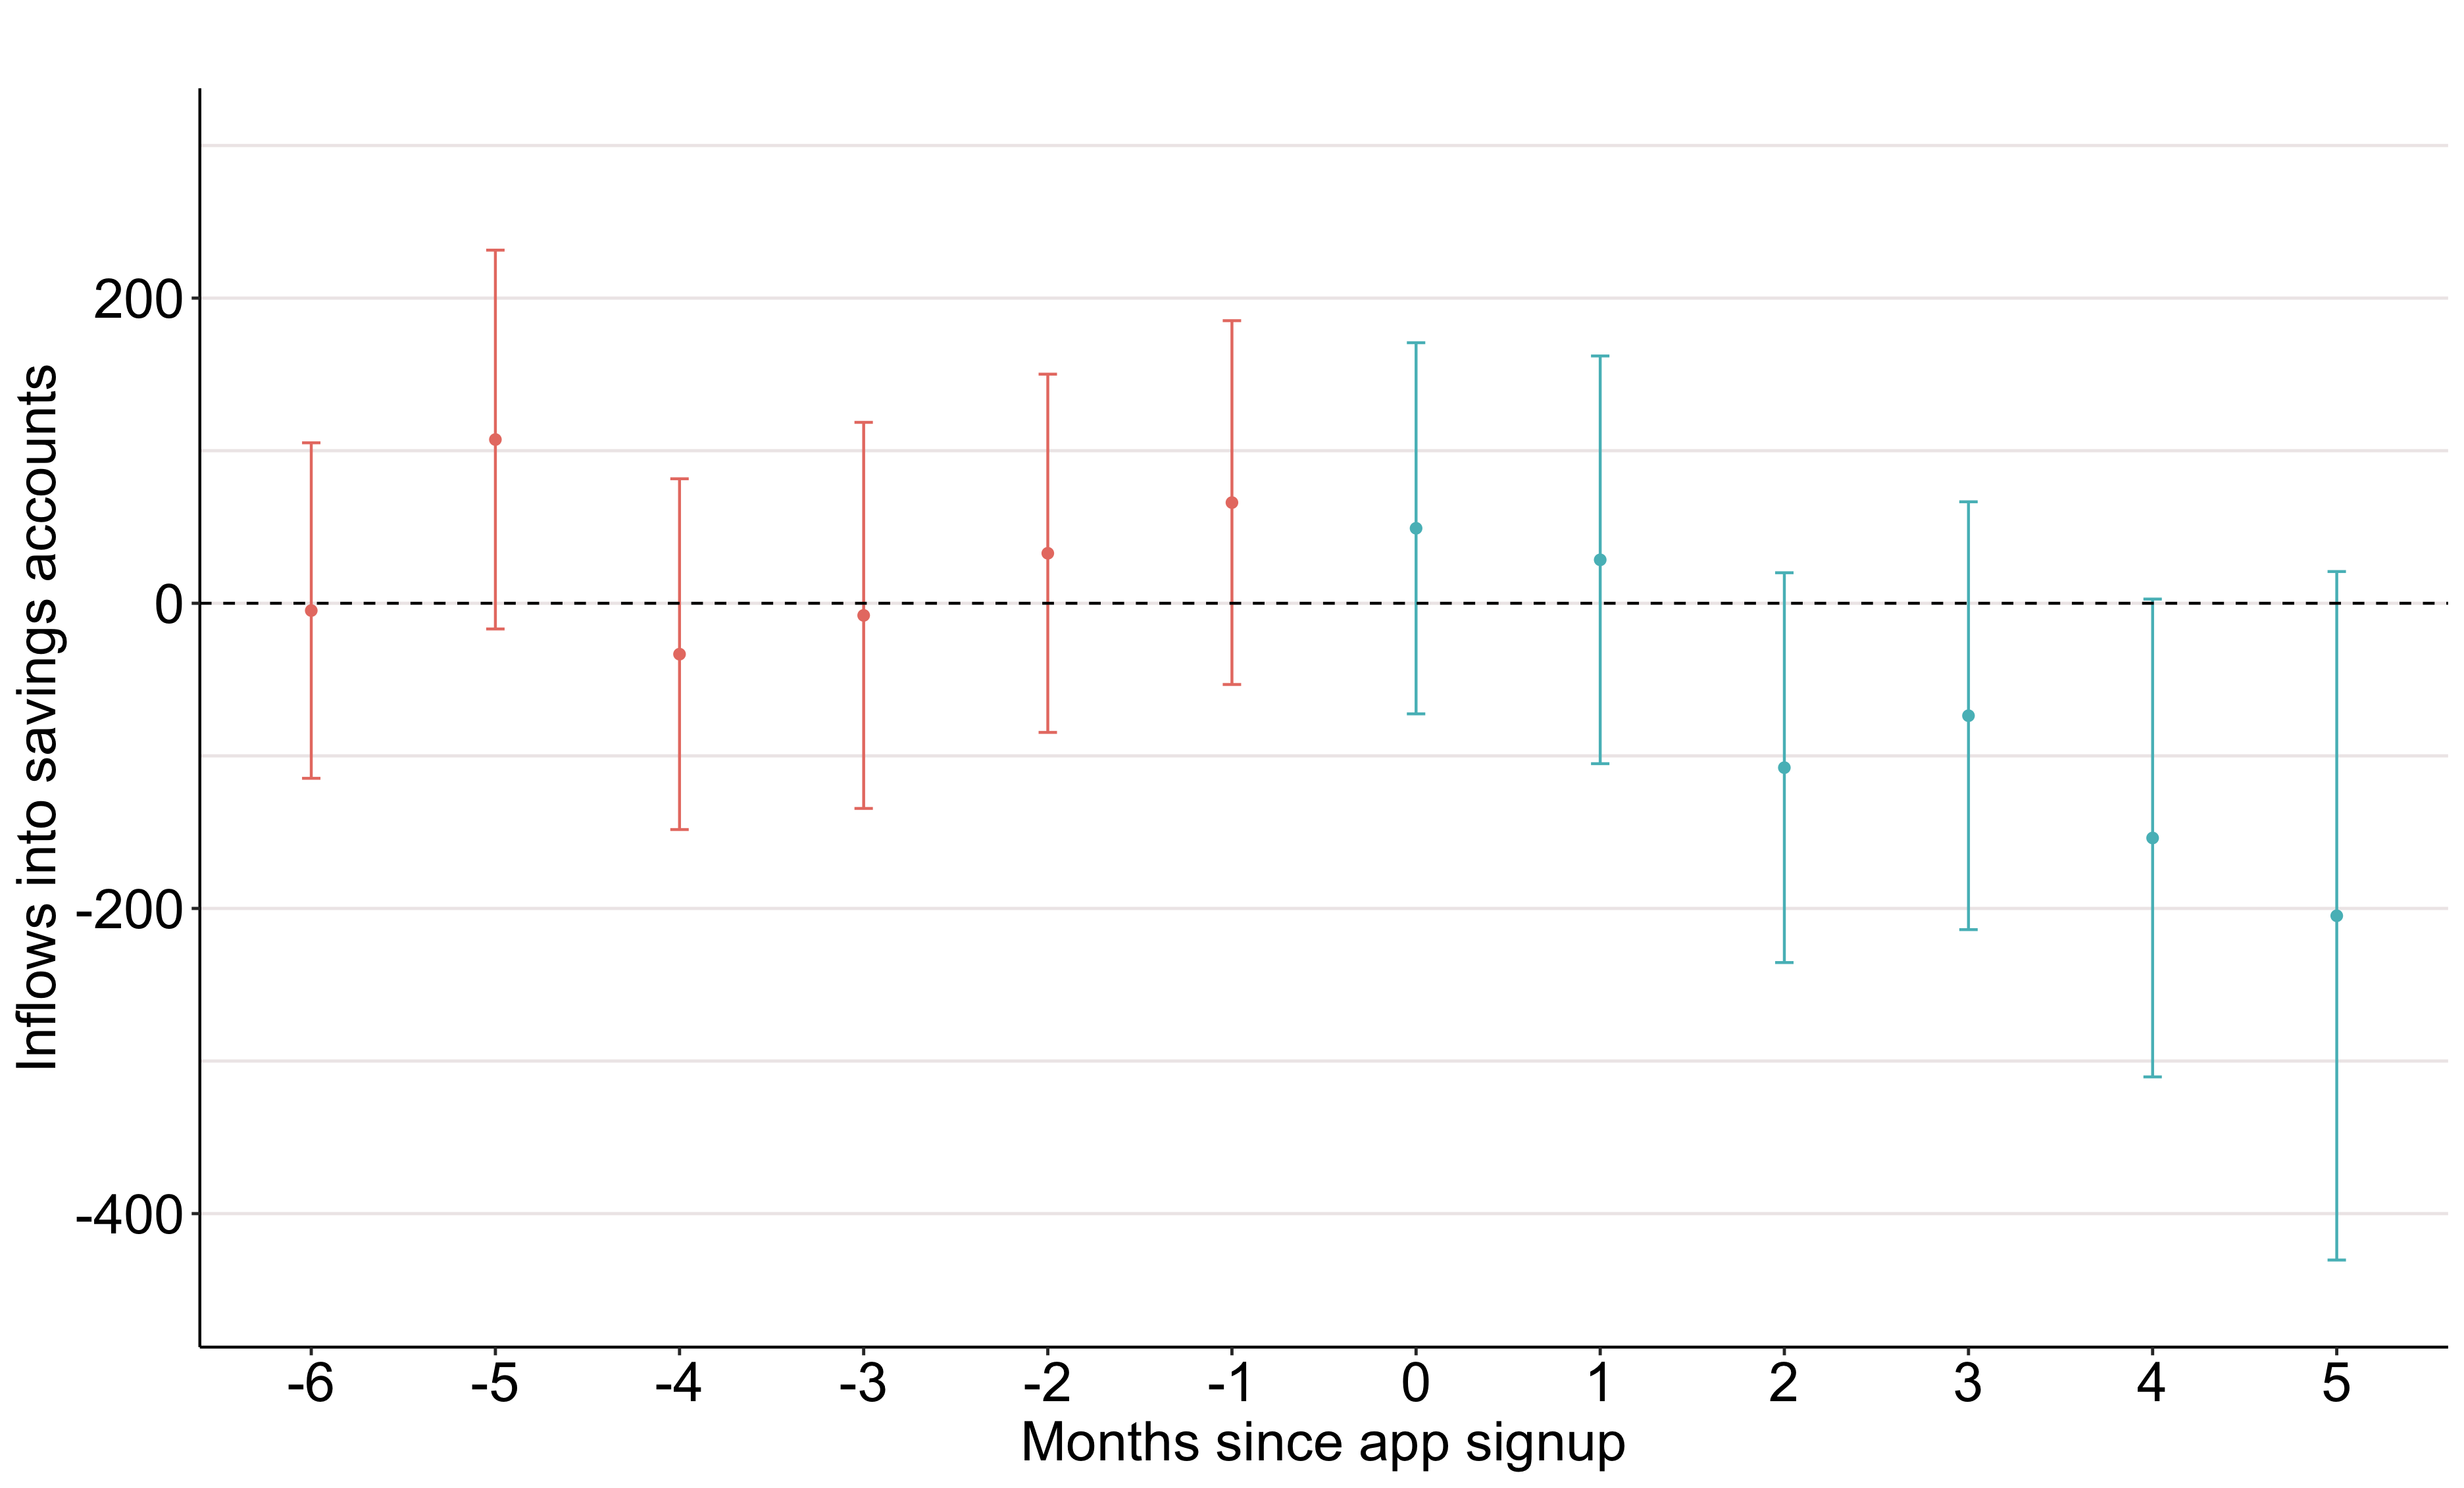
\includegraphics[width=.32\textwidth]{\figdir/inflows_cond_es.png}
    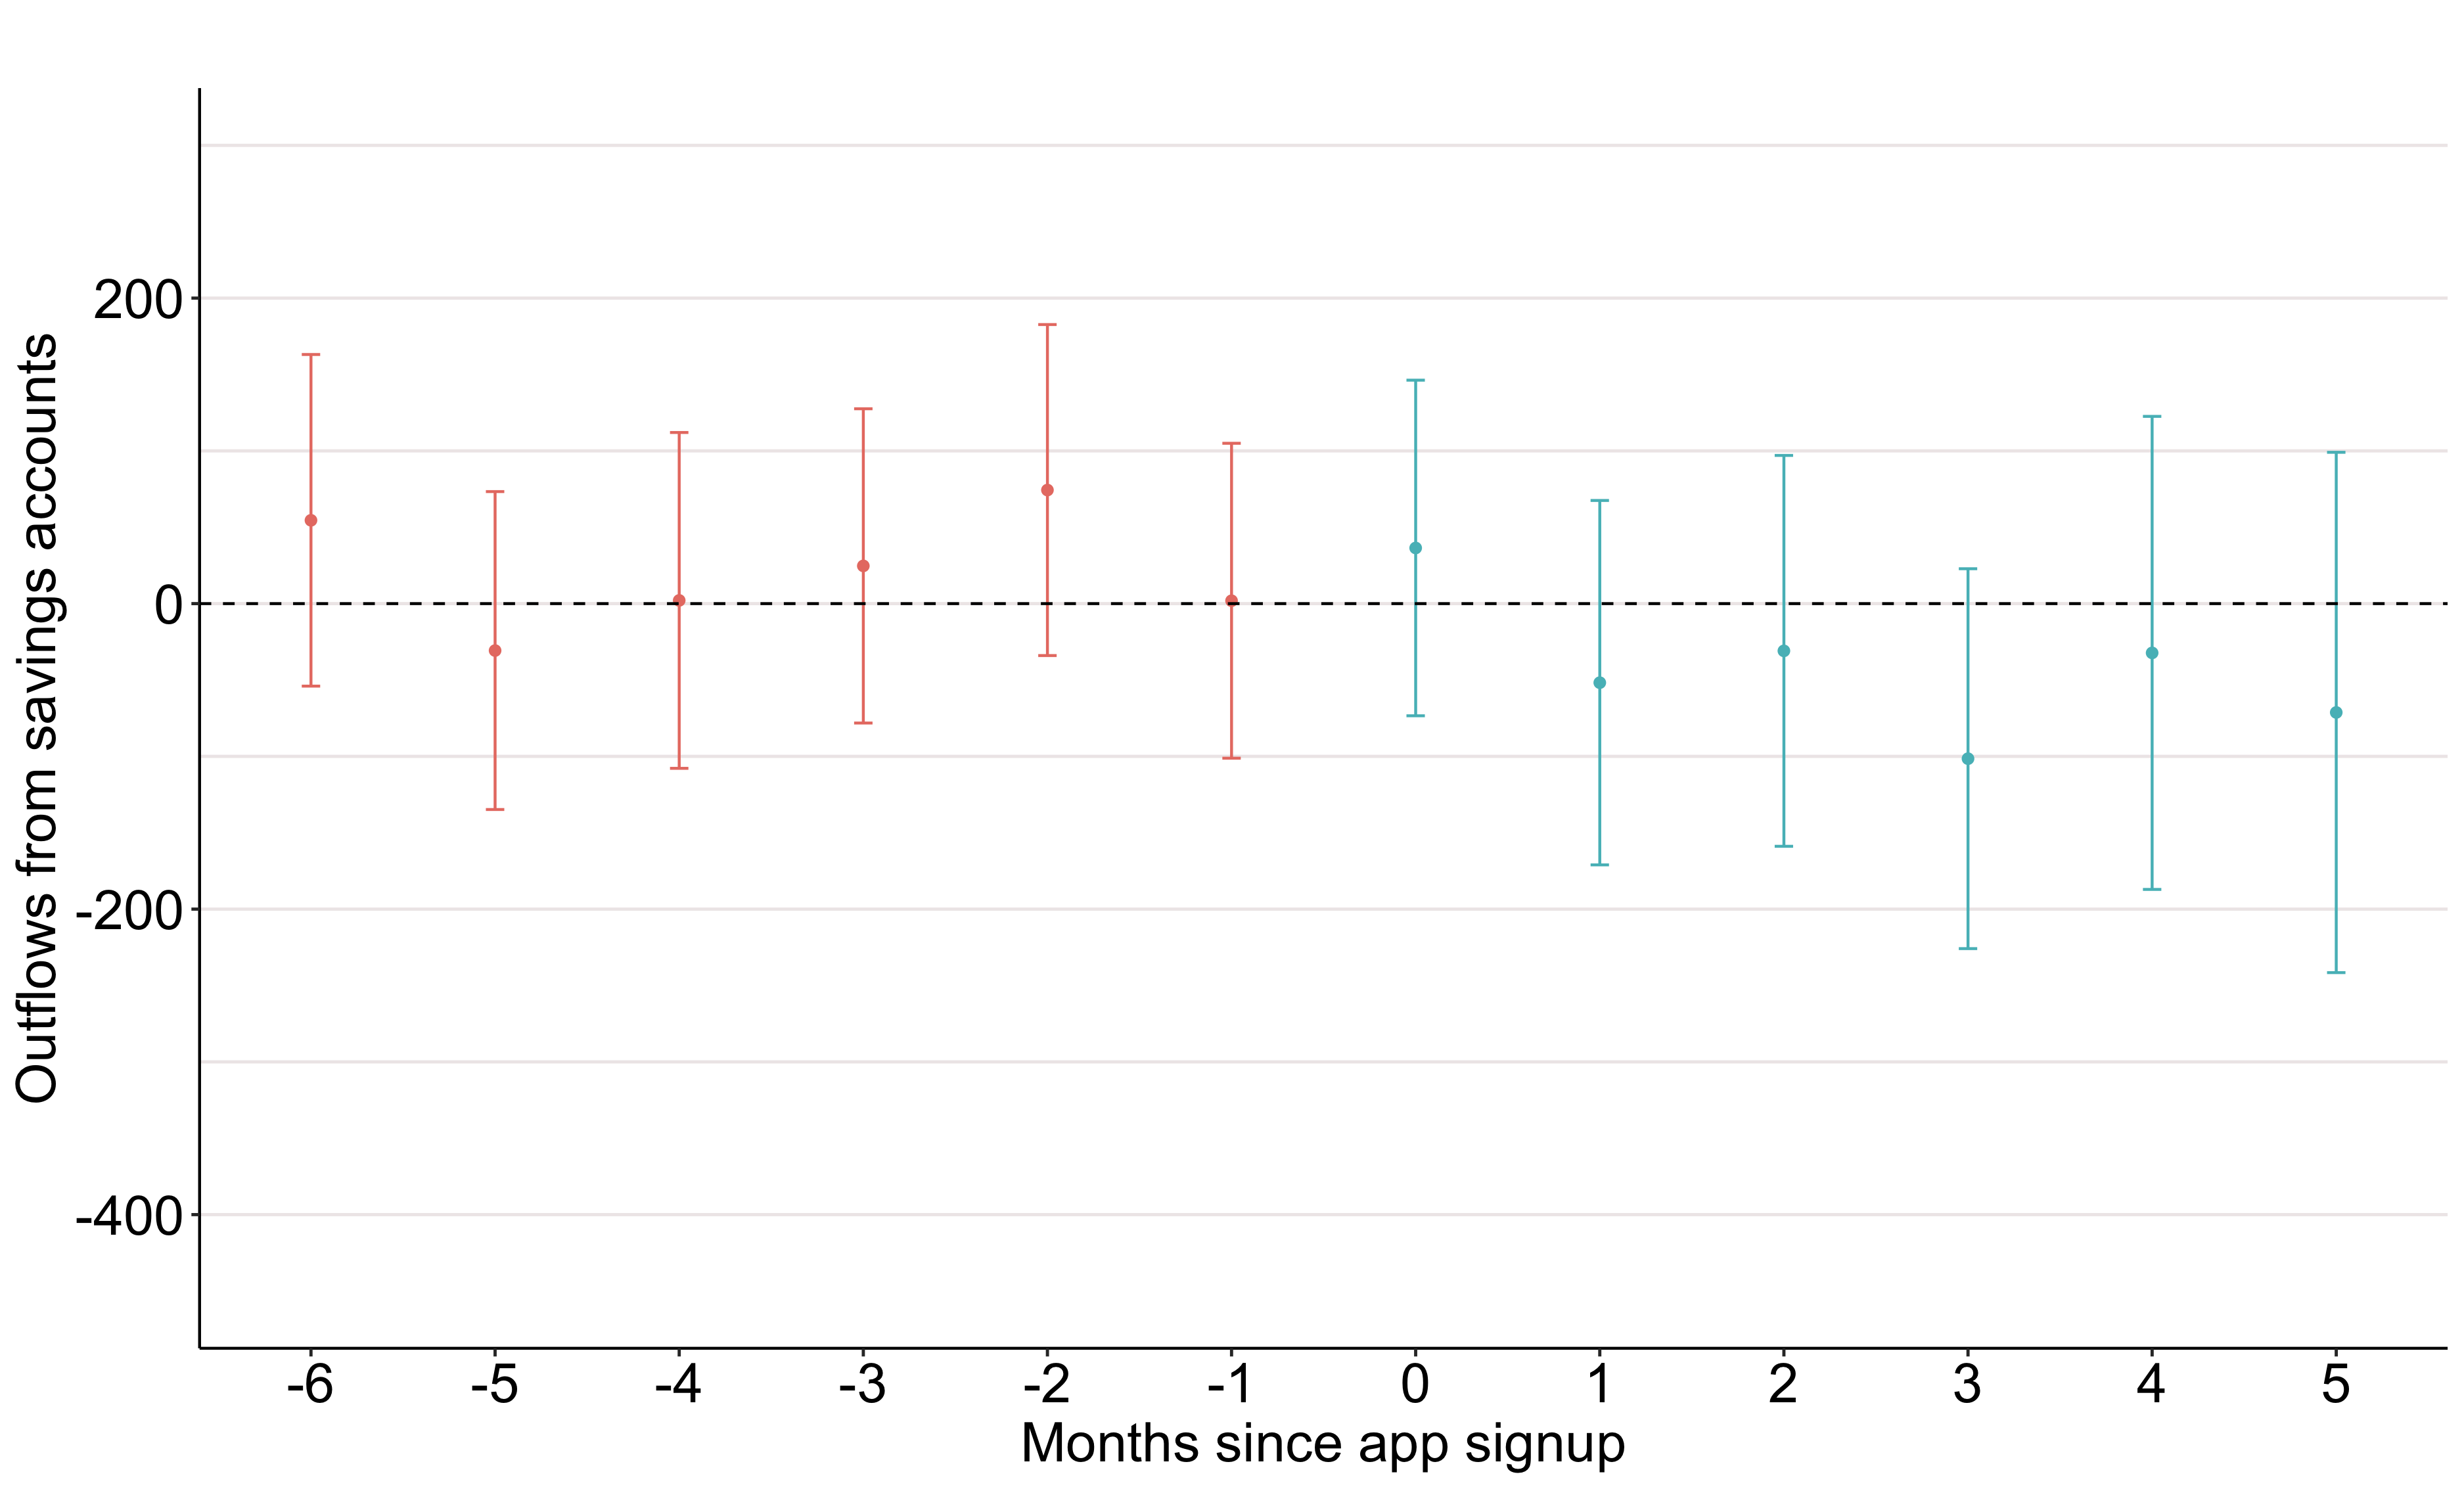
\includegraphics[width=.32\textwidth]{\figdir/outflows_cond_es.png}
    \fignote{\textwidth}{Decomposition of net-inflows into savings accounts
        (left) into inflows (middle) and outflows (right). Point estimates
        represent group-time average treatment effects aggregated to periods
        since treatment exposure, as defined in Section~\ref{sec:estimation}.
        Red lines represent point estimates and uniform 95\% confidence bands
        for pre-treatment periods allowing for clustering at the user level. If
        the null hypothesis that parallel trends hold in all periods is
        correct, these should be equal to zero. Blue lines provide similar
        information for post-treatment periods.}
\end{figure}


\appendix

\section{Money Dashboard application}%
\label{sec:money_dashboard_application}

\begin{figure}[htpb]
    \centering
    \caption{Money Dashboard website screenshot}%
    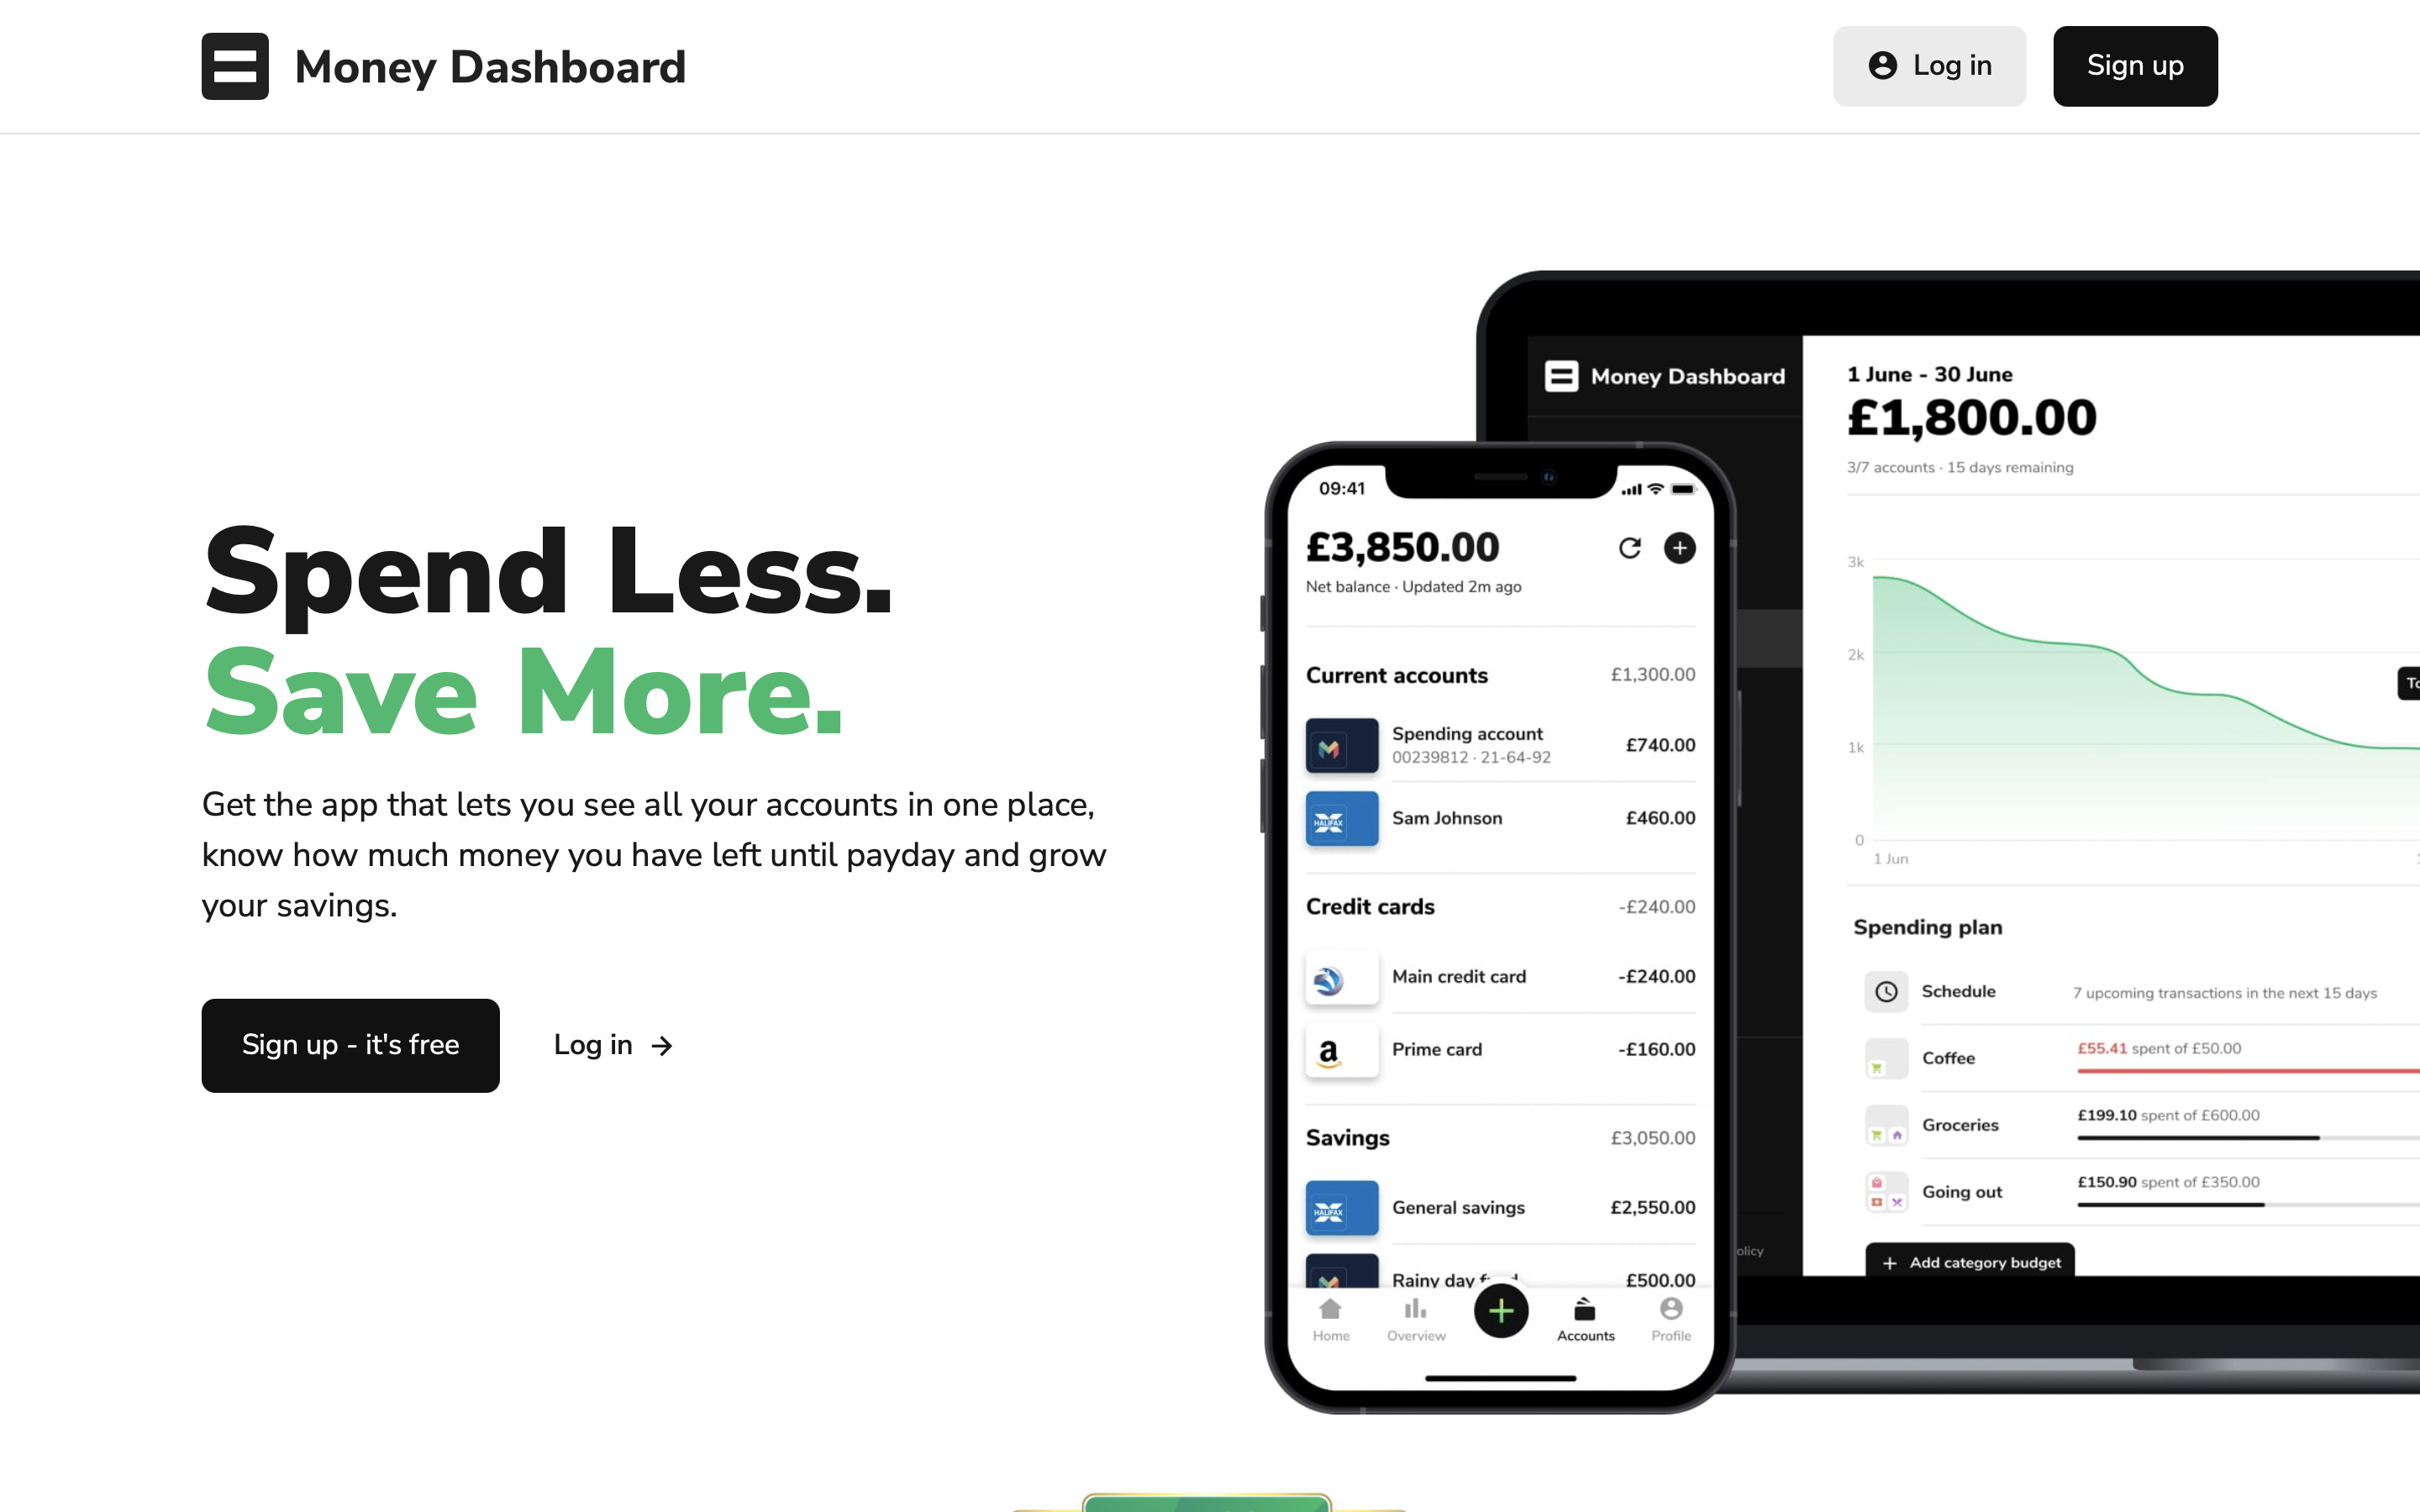
\includegraphics[width=0.8\linewidth]{\figdir/mdb_website}
    \label{fig:mdb_website}
\end{figure}
\fignote{\textwidth}{Screenshot from the top of the Money Dashboard website, at
\href{https://www.moneydashboard.com}{moneydashboard.com}, accessed on 29 April
2022.}

\section{Variable definitions}%
\label{sec:variable_definitions}

Complete steps from raw data to variables used in analysis, with links to code
on Github.


\section{Alternative control group designs}%
\label{sec:alternative_control_group_designs}

\subsection{Alternative window lengths}%
\label{sub:alternative_window_lengths}

Show results for 12 months on either end.

\subsection{Alternative matching method}%
\label{sub:alternative_matching_method}

\subsection{Post treatment periods as control}%
\label{sub:post_treatment_periods_as_control}

\subsection{Synthetic controls}%
\label{sub:synthetic_controls}

\subsection{Classic two-way fixed-effects model}%
\label{sub:classic_two_way_fixed_effects_model}

As discussed in \citet{imai2021matching}.

\subsection{Alternative two-way fixed-effects model}%
\label{sub:alternative_two_way_fixed_effects_model}

Use fixest implementation of \citet{sun2021estimating}.





See \citet{abadie2021penalized} for how to use synthetic controls for
disaggregated data.




\end{document}
